\documentclass[10pt,twocolumn,letterpaper]{article}

\usepackage{iccv}
\usepackage{times}
\usepackage{epsfig}
\usepackage{graphicx}
\usepackage{amsmath}
\usepackage{amssymb}
\usepackage{dsfont}
\usepackage{enumitem}
\usepackage{multicol}
\usepackage{multirow}
\usepackage{amsbsy}
\usepackage{array, caption, floatrow, tabularx, makecell, booktabs}%
\usepackage{animate}
\usepackage{floatrow}
\usepackage{etoolbox}


\setlength{\belowcaptionskip}{-1em}

\iccvfinalcopy % *** Uncomment this line for the final submission

\def\iccvPaperID{4121} % *** Enter the ICCV Paper ID here
\def\httilde{\mbox{\tt\raisebox{-.5ex}{\symbol{126}}}}

% Pages are numbered in submission mode, and unnumbered in camera-ready
\ificcvfinal\pagestyle{empty}\fi

\usepackage{xcolor}
\usepackage[export]{adjustbox}

%%%%%%%%%%%%%%
% Packages and stuff custom
%%%%%%%%%%%%%%
\usepackage{url}
\usepackage{amsthm}
\usepackage{color}
\usepackage{subcaption}
\captionsetup{compatibility=false}
\usepackage{booktabs}
\usepackage{arydshln}
%\usepackage{hyperref}
% If you comment hyperref and then uncomment it, you should delete
% egpaper.aux before re-running latex.  (Or just hit 'q' on the first latex
% run, let it finish, and you should be clear).
\usepackage[pagebackref=true,breaklinks=true,letterpaper=true,colorlinks,bookmarks=false]{hyperref}

\DeclareMathOperator{\E}{\mathbb{E}}
\DeclareMathOperator{\R}{\mathbb{R}}

\def\figref#1{Fig.~\ref{#1}}
\def\secref#1{\S\ref{#1}}
\def\tabref#1{Table~\ref{#1}}
\def\eqnref#1{Eq.~\ref{#1}}

\newcommand{\ow}[1]{\textbf{\textcolor[rgb]{.1, .1, .8}{OW: #1}}}
\newcommand{\rz}[1]{\textbf{\textcolor[rgb]{.54, .16, .55}{RZ: #1}}}
\newcommand{\todo}[1]{\textbf{\textcolor[rgb]{.8, .1, .1}{#1}}}
\newcommand{\pd}[1]{\textbf{\textcolor[rgb]{1, 0.5, 0}{PD: #1}}}
\newcommand{\es}[1]{\textbf{\textcolor[rgb]{0.1, 0.4, 0.1}{ES: #1}}}
\newcommand{\ag}[1]{\textbf{\textcolor[rgb]{0.45, 0.25, 0.1}{AG: #1}}}
\newcommand{\cameraready}[1]{\textcolor[rgb]{0.5, 0.25, 0.15}{#1}}
%% spacehacks
%\setlength{\abovecaptionskip}{-5pt}


\newcommand{\addSubFigHalf}[3]{\begin{subfigure}[t]{.45\linewidth}
   \includegraphics[width=\linewidth]{#1}
   \caption{#2}\label{#3}\end{subfigure}
}
\newcommand{\addSubFigThird}[3]{\begin{subfigure}[t]{.31\linewidth}
   \includegraphics[width=\linewidth]{#1}
   \caption{#2}\label{#3}\end{subfigure}
}
\newcommand{\addSubFigTenth}[3]{\begin{subfigure}[t]{.16\linewidth}
   \includegraphics[width=\linewidth]{#1}
   \caption{#2}\label{#3}\end{subfigure}
}
\newcommand{\addSubFigSixth}[2]{\begin{subfigure}[t]{.12\linewidth}
   \includegraphics[width=\linewidth]{#1}
   \label{#2}\end{subfigure}
}
\newcommand{\addSubFigSixthLabel}[3]{\begin{subfigure}[t]{.12\linewidth}
   %\rotatebox{90}{#2}
   \includegraphics[width=.9\linewidth]{#1}
   \caption{#2}\label{#3}\end{subfigure}
}



\newcommand{\model}[0]{GateGAN}

\DeclareGraphicsExtensions{.pdf,.jpg}

%%%%%%%%%%%%%%%

\graphicspath{ {images/}{syntheticExp/} {final_images/channel_gated/} {final_images/} {paper_images/} }
%%%%%%%%%%%%%%%%


% Include other packages here, before hyperref.

% If you comment hyperref and then uncomment it, you should delete
% egpaper.aux before re-running latex.  (Or just hit 'q' on the first latex
% run, let it finish, and you should be clear).
\usepackage[pagebackref=true,breaklinks=true,letterpaper=true,colorlinks,bookmarks=false]{hyperref}

% \cvprfinalcopy % *** Uncomment this line for the final submission

\def\iccvPaperID{4121} % *** Enter the CVPR Paper ID here
\def\httilde{\mbox{\tt\raisebox{-.5ex}{\symbol{126}}}}

% Pages are numbered in submission mode, and unnumbered in camera-ready
\ificcvfinal\pagestyle{empty}\fi
\begin{document}

%%%%%%%%% TITLE
\title{Interactive Sketch \& Fill: Multiclass Sketch-to-Image Translation}
%\title{Interactive Sketch and Fill: Multiclass Outline-to-Image with Gated Residual Networks}
%\title{Complete and Translate: Multiclass Outline-to-Image with Gated Residual Networks}
% \title{GAN-Gate: Gated Residual GANs for Class-Conditioned Image Generation}
% GAN-Gate: Conditionally-Gated Residual Networks for Image-to-Image Translation
% GAN-Gate: Softly-Gated Conditional Residual Networks for Image-to-Image Translation
% GAN-Gate: Conditionally Soft-Gated Residual Networks for Image-to-Image Translation
%GAN-Gate: Conditional Gating for Image-to-Image Translation

% \author{Arnab Ghosh\\
% University of Oxford\\
% {\tt\small arnab.ghosh@eng.ox.ac.uk}
% % For a paper whose authors are all at the same institution,
% % omit the following lines up until the closing ``}''.
% % Additional authors and addresses can be added with ``\and'',
% % just like the second author.
% % To save space, use either the email address or home page, not both
% \and
% Richard Zhang\\
% Adobe Research\\
% {\tt\small rizhang@adobe.com}
% \and
% Puneet Dokania\\
% University of Oxford\\
% {\tt\small puneet@robots.ox.ac.uk}
% \and
% Oliver Wang\\
% Adobe Research\\
% {\tt\small owang@adobe.com}
% \and
% Alexei A. Efros\\
% UC Berkeley\\
% {\tt\small efros@eecs.berkeley.edu}
% \and
% Philip Torr\\
% University of Oxford\\
% {\tt\small philip.torr@eng.ox.ac.uk}
% \and
% Eli Shechtman\\
% Adobe Research\\
% {\tt\small elishe@adobe.com}
% }

% \author{
% Arnab Ghosh$^1$, Richard Zhang$^2$ , Puneet K. Dokania$^1$ ,\\
% Oliver Wang$^2$,  Alexei A. Efros$^2^,^3$, Philip H.S. Torr$^1$, Eli Shechtman $^2$ \vspace{5pt} \\
% $^1$University of Oxford \quad $^2$Adobe Research \quad $^3$ UC Berkeley \vspace{5pt} \\ 
% {\tt \{arnabg,puneet,phst\}@robots.ox.ac.uk,\{rizhang,owang,elishe\}@adobe.com}, \\ {\tt efros@eecs.berkeley.edu}
% }

\author{
Arnab Ghosh$^{1}$ \hspace{8mm} Richard Zhang$^{2}$ \hspace{8mm} Puneet K. Dokania$^{1}$ \\
Oliver Wang$^{2}$ \hspace{8mm} Alexei A. Efros$^{2,3}$ \hspace{8mm} Philip H. S. Torr$^{1}$ \hspace{8mm} Eli Shechtman$^{2}$ \\
\\
$^{1}$University of Oxford \hspace{15mm} $^{2}$Adobe Research \hspace{15mm} $^{3}$UC Berkeley \\
% Arnab Ghosh$^{1}$ \hspace{6mm} Richard Zhang$^{2}$ \hspace{6mm} Puneet K. Dokania$^{1}$ \hspace{6mm} Oliver Wang$^{2}$\\
% Alexei A. Efros$^{2,3}$ \hspace{6mm} Philip H. S. Torr$^{1}$ \hspace{6mm} Eli Shechtman$^{2}$ \\
% \\
% $^{1}$University of Oxford \hspace{2.3cm} $^{2}$Adobe Research \hspace{2.3cm} $^{3}$UC Berkeley \\
% {\tt\footnotesize \{arnabg,puneet,phst\}@robots.ox.ac.uk \hspace{2mm} \{\tt\footnotesize rizhang,owang,elishe\}@adobe.com} \hspace{2mm} {\tt\footnotesize \{efros\}@eecs.berkeley.edu}
% \vspace*{-2mm}
}

% \author{Richard Zhang$^{1}$ \hspace{3mm} Phillip Isola$^{12}$ \hspace{3mm} Alexei A. Efros$^{1}$\\
% $^{1}$UC Berkeley \hspace{3mm} $^{2}$OpenAI\\
% {\tt\small \{rich.zhang, isola, efros\}@eecs.berkeley.edu}
% \and
% Eli Shechtman$^{3}$ \hspace{3mm} Oliver Wang$^{3}$\\
% $^{3}$Adobe Research\\
% {\tt\small \{elishe,owang\}@adobe.com}
% }

%\maketitle
%\thispagestyle{empty}


\twocolumn[{%
\renewcommand\twocolumn[1][]{#1}%
\maketitle
\begin{center}
    \centering
    % 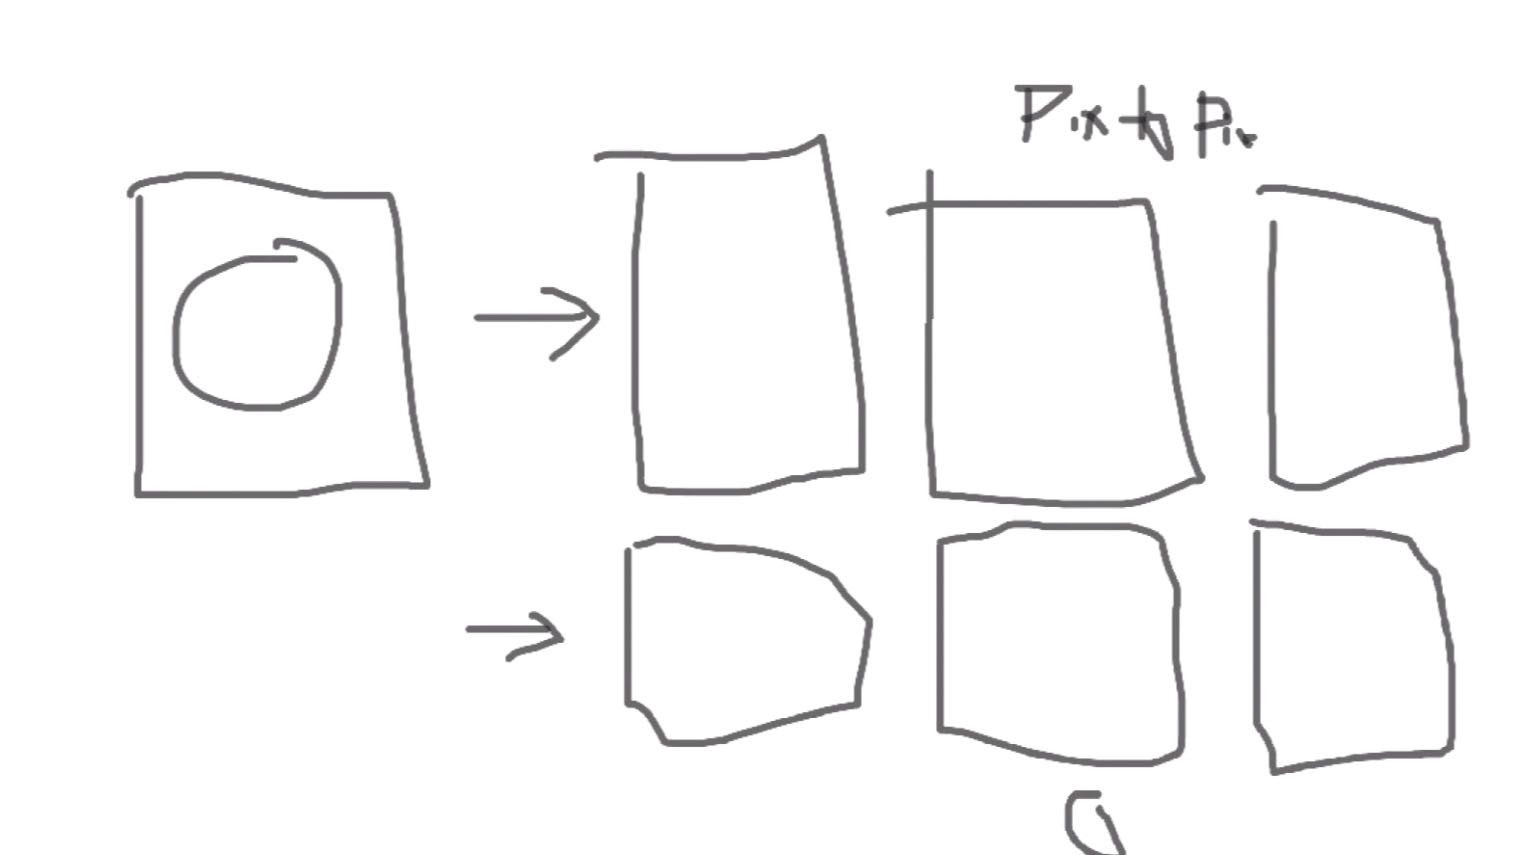
\includegraphics[width=.9\linewidth,height=4.5cm]{images/teaser/sketch.jpg}
    % 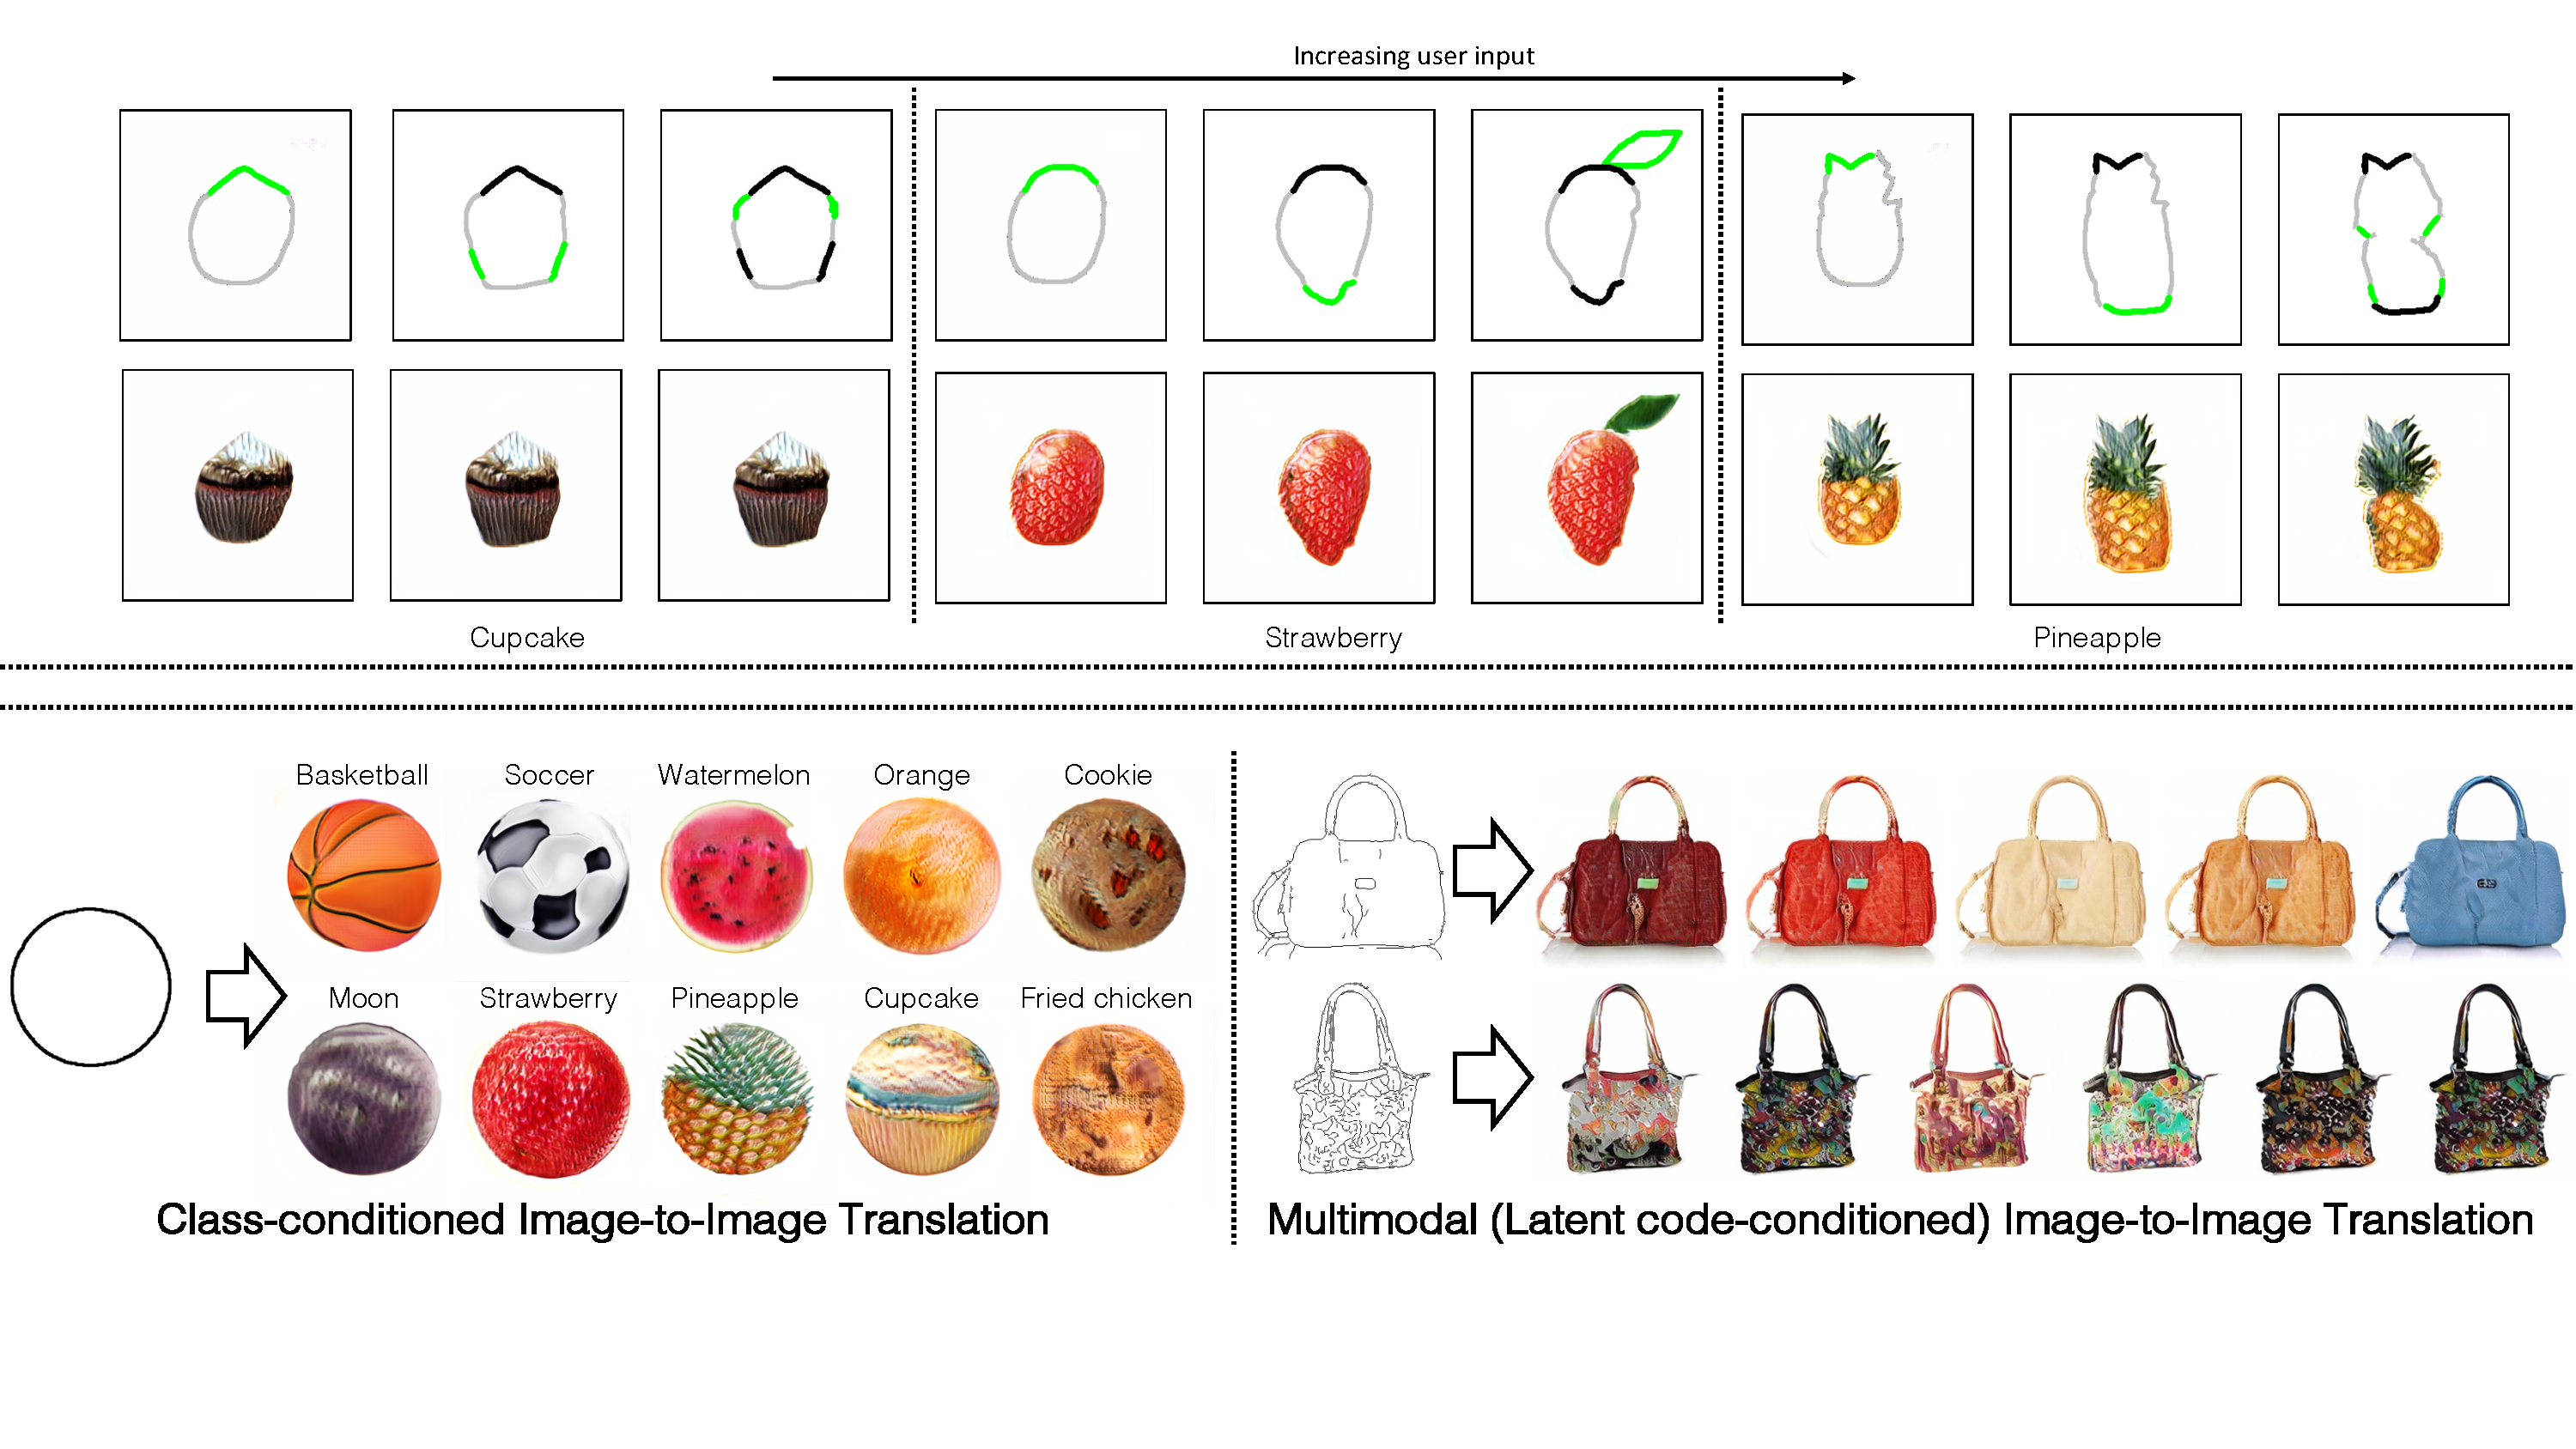
\includegraphics[width=1.\linewidth]{paper_images/teaser_autocomplete_v4.pdf}
    % \vspace{-20mm}
    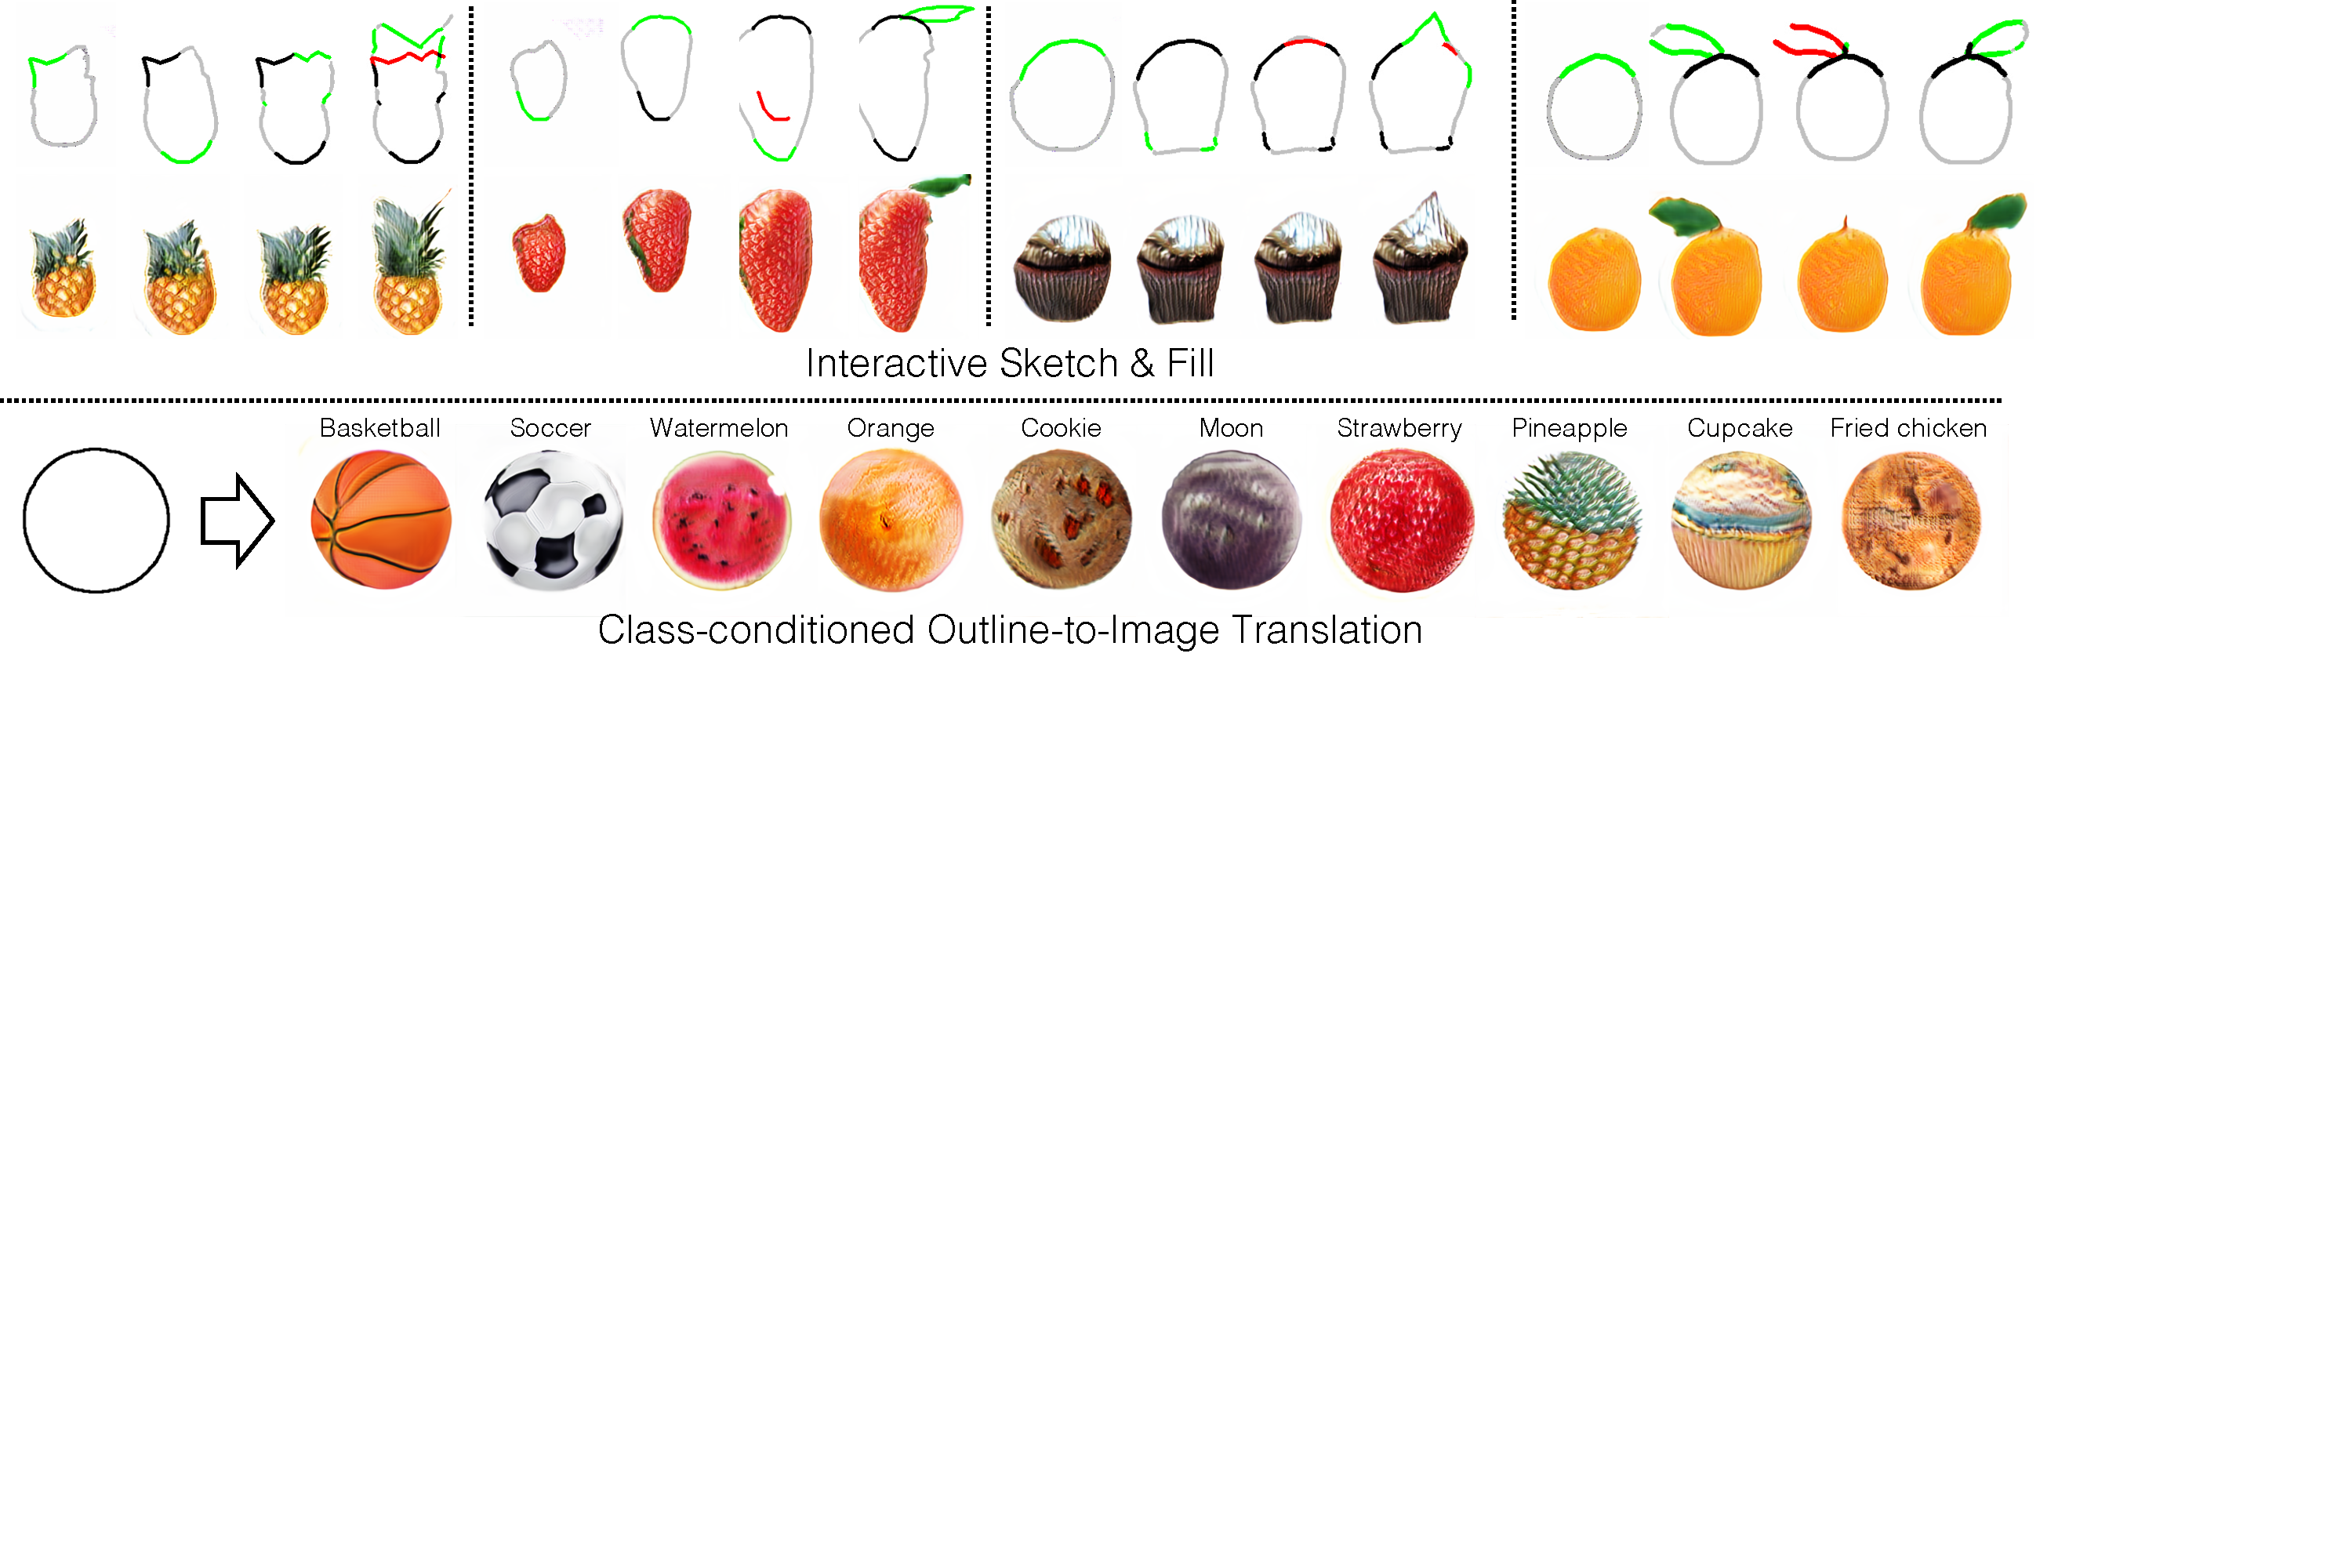
\includegraphics[width=1.\linewidth]{paper_images/teaser_v7.pdf}
    
    \captionof{figure}{({\bf Top}) Given sparse user input (first row), our model estimates the complete shape and provides this as a recommendation to the user (shown in gray), along with the final synthesized object (second row). These estimates are updated as the user adds strokes over time (shown in \textcolor{green}{green}), or removes strokes (shown in \textcolor{red}{red}) -- previous edits are shown in black.
    ({\bf Bottom}) This generation is class conditioned, and our method is able to generate distinct multiple objects for the same outline (\eg `circle'), by conditioning the generator on the object category.\label{fig:teaser}
    }
    \vspace{1em}
\end{center}%
}]
    
%%%%%%%%% ABSTRACT
\begin{abstract}
We propose a new task involving GAN based recommender that helps novice users to interactively synthesize images of simple objects merely using partial sketches.
The user starts with an extremely sparse sketch for the object category as an input, and the network then recommends its plausible completion and shows corresponding synthesized image. This allows the user to interactively take feedback from the network, edit the input sketch, and synthesize the desired object.
In order to be able to use a single model for a wide array of object classes, we introduce a gating based approach for class conditioning, which allows us to generate distinct classes without feature mixing, from a single generator network.

%Effectively incorporating low-dimensional conditioning is a crucial, yet relatively unexplored, aspect of multiclass, multimodal, and multitask image-to-image translation.
%We systematically investigate variants of injecting conditioning into GAN architectures. We propose a soft-gating mechanism, which learns to ``select" which parts of a ResNet~\cite{he2016deep} are used, based on the conditioner.
%We validate on a challenging outline-to-image task, mapping from a sparse sketch with no internal structure. 
%Class conditioning is especially important, and the soft-gating mechanism enables plausible generations where naive concatenation fails.
%The method is also effective on standard sketch-to-image and day-to-night tasks.
%Additionally, the gating better fulfills the InfoGAN~\cite{chen2016infogan} objective, maximizing mutual information between the output and the conditioner,
% in an effective way,
%enabling diverse generations for image-to-image translation. 
% We demonstrate that our approach is able to generate high quality multiclass image translations, outperforming prior state-of-the-art methods.

%We propose a method that allows us to generate images belonging to multiple domains using a single network.
%Our approach is based on a GAN framework with two separate branches, a fully residual generator and discriminator, and a separate smaller gating network.
%The gating network selects residual blocks from the generator and discriminator based on some conditioning.
%We show that such an approach is able to produce high quality multi-class image generation, both in an class-conditioned image-to-image translation task, as well as in an unsupervised image generation task where diversity is learned.
%This method allows for significantly smaller model sizes than previous multi-class approaches by taking advantage of similarities across classes. 
%We analyze our gating network to show that it leads to subnetworks based on the residual blocks that are active for a particular class.
%This approach as well as helps inject low dimensional information into a network more effectively than just concatenating channel-wise after replication to match the image dimension. 
%Information theoretic results also show it to be a much stronger form of conditioning than naive concatenation. 
%We apply our approach on a novel setting of multi-class outline-to-image generation, where baseline solutions fail to generate good results, while our model successfully tackles the multi-class image generation setting. 
\end{abstract}




\section{Introduction}
%Deep generative models have seen incredible progress in terms of generating realistic images from random noise \cite{brock2018large}, \cite{karras2018style}.
%Deep generative models using Generative Adversarial Nets (GANs) have shown remarkable promise for being able to generate realistic mappings between image domains, for example semantic labels\cite{isola2016image2image}, and edges~\cite{zhu2017unpaired}.
%\pd{talk more about it, references are not enough.}
%\ow{need to state the problem with these that we are solving}
%\es{Here is how I would start:}

Conditional GAN based image translation \cite{isola2016image2image,sangkloy2017scribbler,zhu2017unpaired} models showed remarkable success at taking an abstract user input such as an edge map or a semantic segmentation map and translating it to a real image. These methods run at interactive rates and combining them with a user interface allows the user to quickly create funny (unreal) looking images\todo{cite}. However, a few limitations prevent them from being used as a true interactive tool that assists the user in generating an image of an object they have in mind. First, the user is required to provide an entire abstract map as input (full edge or label map) which could be hard for many users as it is known that average people are not good at free-hand drawing of accurate proportions of objects and their parts~\cite{}, 3D shapes and perspective~\cite{ }. It is much easier with current image translation methods to obtain realistic looking images by editing existing images \cite{dekel2018sparse,portenier2018faceshop} ~\cite{ } than creating images from scratch. Second, current GAN-based image translation methods are limited to a single class of images. Switching from drawing a cat to a dog requires loading (or storing in memory) a new model per class.

We propose a new GAN-based interactive image generation system that: 1) generates full images from {\em sparse} and {\em partial} user strokes as input; 2) serves as a \emph{recommender system} that suggests or helps the user, \emph{during} their creative process, in order to generate a desired image; and 3) uses a single conditional GAN for {\em multiple} image classes with an effective gating mechanism. Such a system allows for creative input to come from the user, while the challenging task of getting exact proportions correct is left to the GAN-based agent, who constantly predicts a plausible completion of the user stroke and a plausible image configuration related to that. 
%These two suggestions or recommendations from the GAN agent will help the user to adapt the stroke depending on the type of object it is interested in.
%In that context, our system learns mapping from the domain of easy-to-give user input (e.g., sparse strokes), to realistic images, while giving feedbacks to the user.
%In this feedback loop, the user takes inspiration from the \emph{and} the learned model each condition their next steps based on the previous output of the other. 

To address the first limitation of the above mentioned system we replace dense edge maps with sparse object outlines as the input representation, as outlines are closer to lines that novice users tend to draw than dense edge maps \cite{cole2008people}. We then train our model to first complete partial outlines to full ones and then generate the image conditioned on the completed outlines. We found this to work better than going directly from partial outlines to full images as the additional intermediate supervision on full outlines breaks the problem into two easier sub-problems -- first recover the geometric properties of the object (shape, proportions) and then fill-in the appearance (colors, textures). 

There are several advantages to this two-stage approach.
For one, we are able to give the artist feedback of the general object shape in our interactive interface (similar to \cite{lee2011shadowdraw}), allowing them to quickly refine the completed shape until it is satisfactory.
Second, by separating the problem into two steps, we have greatly simplified the training challenge. We show in Sec.~\ref{sec:experiments} that sequential stroke completion followed appearance prediction is much more stable to train than predicting the appearance directly from partial strokes.

Multi-class conditional generation is achieved using a novel gating mechanism conditioned on the input class label. Briefly, gating allows the network to focus on the important parts (or activations) of the network specific to the conditioning. Such an approach allows for a clean separation of classes, enabling us to train a single generator and discriminator to cleanly generate \emph{multiple} object classes based on this gating conditioning.

To demonstrate the potential of our method as an interactive tool for stroke-based image generation we collected a new dataset of ten image classes. We focus on simple object classes on white backgrounds although we believe our method is general and can be applied for other image types and other types of sparse strokes. In order to stress test our gating mechanism, six (basketball, soccer, watermelon, orange, cookie, moon) of the objects had similar round outlines so the model is truly conditioned on the class label and cannot figure out the class only from the strokes. \pd{not sure: In addition, we also show that the gating helps infoGAN in learning multi-modal distribution for image to image translation task, which otherwise requires sophisticated models such as BicylceGAN, MAD-GAN,...}

%In this work, we investigate using image-to-image translation in an interactive interface, where the network predictions serve as a \emph{recommender system} that suggests or helps the user, \emph{during} their creative process, in order to generate a desired image (Fig.~\figref{fig:teaser}). 
%In that context, we are interested in mapping from the domain of easy-to-give user input (e.g., sparse strokes), to realistic images.
%Such a system allows for creative input to come from the user, while the challenging task of getting exact proportions correct is left to the GAN-based agent, who constantly predicts the most plausible image configuration given the users inputs. 
%In this feedback loop, the user \emph{and} the learned model each condition their next steps based on the previous output of the other. 

%For example, imagine a scenario where a user wants the system to synthesize a real image of an object, say `strawberry', merely from the outline. 
%n this case, it is too much to expect from the user to first draw the complete outline of the strawberry, and then ask the system to generate real images respecting the geometry of the outline. 
%This would require the user to have a complete understanding of the shape of the strawberry. 
%However, a more user-friendly system would be the one where the user gives a {\em partial outline}, like a starting point, of the strawberry as an input, and the system then recommends a plausible {\em completion} of the outline (specific to strawberries) and a synthesized image corresponding to that completion. This would help the user to take feed-backs from these two suggestions from the system, the complete outline and the synthesized image, and then keep on drawing the outline without the need of any external intervention or prior knowledge of the shape of the strawberry.
%In order to train such a system, we split the problem of mapping sketches to images into two stages: a \emph{geometric} completion stage, followed by a \emph{texture} completion stage. 
%Even though the above mentioned task is extremely useful in practice, no work has been done in this direction from generative modelling point of view \pd{not sure if we can write this.}. 
%Furthermore, there are two main problems towards achieving a practical system -- (1) depending on the object category, a partial outline can have multiple completions; and 2) given a complete outline, again, multiple textures can be synthesized, depending on the desired object type. 
%We provide a  simple and intuitive solution to these problems by using a conditional \emph{gating} approach. As shown in \todo{fig}, gating allows the network to focus on the important parts (or activations) of the specific to the conditioning. 
%Such an approach allows for a clean separation of classes, enabling us to train a single generator and discriminator to cleanly generate \emph{multiple} object classes based on this gating conditioning.
%We discuss this in detail in Section..  \pd{not sure if this is the right place to talk about gatings etc.}
%Furthermore, we provide information theoretic explanation behind the efficacy of gating, and show that this simple modification to the architecture even allows {\em infoGAN} to learn multi-modal distribution for the image to image translation task, which otherwise requires sophisticated approaches such as BicycleGAN and MAD-GAN.
%We create a dataset for the above said task and will release it for public use. 
%In addition to proposing gating as a potential solution to the task, we also show that gating, in fact, allows the network to efficiently utilize its capacity which in turn allowed us to train a single GAN to perform image generation on multiple object categories. 

%In detail,where the condition is a {\em partial outline} or {\em strokes}, and the objective is to first suggest or recommend a completion of this partial outline, depending on the object category we are interested in, and then, based on the completion, generate a realistic image (refer~\figref{fig:teaser}). In contrast to `edges' to `image' generation, this task is more useful in practice because of various obvious reasons -- (1) as opposed to outlines, edges require filling the internal structure (captures semantic information as well) with high precision which is an extremely tedious task when it comes to developing a user-friendly system, and (2) drawing partial outlines are easier and a `object-specific' auto-completion will help the user to complete the outline with precision.

%Conservatively speaking, there are two main problems associated with the above said problem: 1) depending on the object category, a partial outline can have multiple completions; and 2) given a complete outline, again, multiple images can be synthesized from it depending on the object category.  We provide extremely simple and intuitive solutions to these problems, a crucial ingredient to which is the {\em gatings} introduced in the ResNet based GAN generator and discriminator architectures. We show that naive use of standard GAN is not enough to address these issues, and, propose fully residual block based discriminator and generator with {\em gatings} as a solution for that. Briefly, as shown in , gating allows the network to focus on the parts (or activations) of the network which is crucial for the given condition.   \pd{not sure if this is the right place to talk about gatings etc.}

%\pd{not sure}
%To address the first issue, we propose a data-driven approach where we curate dataset with pairs of partial-outlines and corresponding images, and use BicycleGAN type training with gated discriminator and generator to learn such mappings. Note, a naive approach of using a pix2pix architecture failed in this setting. Similarly, we design  

%\pd{notes: partial outlines lead to real time, two stage process as single didn't work, partial to full outlines was trained using Gated-Bicycle GAN as normal GAN (pix2pix) or BiCycle GAN didnt work directly. BiCycle worked for single class, but pix2pix didn't even work for single. Arnab isn't sure if Bicycle with simple concatenation would work or not.}

%There is a void left between the non image conditional setting and the image conditional setting in which only a few user guidelines should condition the image generation. 
%\ow{danger: iGAN, FaceShop, SketchyGAN}
%\pd{do we need this? too much i think}
%Controllable Generations could be more important since users associate more with products they helped partially create which has been studied by cognitive psychologists and termed as the IKEA effect \cite{norton2012ikea}. 

%User guided image synthesis is an important application case for GAN technology, however previous solutions have properties that make user interation non-intuitive. For example, they generate high quality images from random noise vectors~\cite{brock2018large,karras2018style}, or they generate images from edge maps~\cite{isola2016image2image,zhu2017unpaired}. \ow{same problem with the partial methods above, need to make our contributions more unique}
%In this work, we address the user-guided image generation problem by proposing a new dataset of image outlines, and train a two stage model whereby user input is first completed then translated into images. 
%We also propose a gated GAN model to handle class conditioning for the generated images, allowing us to generate multiple classes using the same model..

%In pursuit of collaborative image generation between user and the machine we introduce a system whereby a user can generate real looking objects from a few strokes, whereby a network first automatically completes the strokes for the user honoring the user's strokes and another network generates images conditioned on the completed stroke image.

%A naive solution might be to complete the image from the incomplete edge map to the final image but turns out that the generation of realistic images from partial edge maps is quite difficult for current systems. 
%Another option could be to completing the edge maps themselves but current systems fail at that as well.

%\pd{not sure}
%Completing the outlines of the images turns out to be relatively much easier task, and we demonstrate on multiple settings the efficacy of our models on the task of completing outlines. Traditional pix2pix systems were designed to go from one input sketch to 1 output class of bags or shoes but in general objects come in multiple different shapes and several of those outlines could be similar and hence the low dimensional class information has to be properly injected into the network. Naive concatenation techniques demonstrates an innate problem of image conditional neural networks whereby the class conditioning fails to work in several settings. To mitigate the issue of conditioning of the image conditional networks we use class conditioned gating of the residual blocks for better conditioning.


%Sketch RNN \cite{ha2017neural} was an attempt in that direction but required the intermediate stages of the sketches while training which is not always available. iGAN \cite{zhu2016generative} was a step in the direction of making GANs interactive but used a complex optimization based technique to obtain the closest image.

% \section{Introduction}
% Generative methods have made huge strides in the last few years, driven by the success of models such as Generative Adversarial Networks (GANs)~\cite{goodfellow2014generative} and Variational Autoencoders (VAEs)~\cite{kingma2013auto}.
% % These methods can generate impressive results, but
% One major challenge is that quality can degrade when the diversity of training data increases.
% % (e.g., number of object/scene classes).
% A common practice in conditional image conditional generation is to train different models for different tasks~\cite{isola2016image2image,karras2017progressive,zhu2017toward,zhu2017unpaired,wang2017high,wang2018video}, meaning that parameters scale linearly with the number of tasks.
% %However their proposed method still involved training multiple generators.
% % A study performed in \cite{ghosh2017multi,metz2017unrolledGAN} demonstrated that even in a simple 1D \& 2D Mixture of Gaussians settings, state-of-the-art GAN techniques were not able to generate samples from all the components of the mixture. 
% This presents an intriguing opportunity -- ideally, a single network can solve multiple tasks. Such a network would have the flexibility to share operations applicable across tasks, while dedicating resources responsible for task-specific operations.
% % An ideal scenario in such settings would involve a single network which could share parts responsible for similar operations across classes while unsharing the discrete parts of the network which are responsible for class specific operations.

% % Such a scenario was analyzed in the realm of
% In image classification, Veit et al.~\cite{veit2016residual} show, through lesion experiments, that a Residual Network~\cite{he2016deep} implicitly allows information flow through multiple paths. Follow-up work~\cite{veit2018adaptive} aims to explicitly specialize different paths for different classes~\cite{veit2018adaptive}.
% % In image classification, Veit et al.~\cite{veit2016residual} perform incision experiments on a pretrained ResNet architecture~\cite{he2016deep}, demonstrating that certain paths in the network play a more important role for certain classes.
% %inferring that ResNets behave like an ensemble of several partially disjoint networks for image classification. 
% In this paper, we analyze the implications of this observation in a generative modeling scenario. 
% We analyze GANs on a 1D Mixture of Gaussians distribution, as used in~\cite{ghosh2017multi}, and discover that removal of blocks corresponds to the disappearance of certain modes in the generated distribution.

% Motivated by this, we introduce a simple {\em soft-gating} mechanism, where a hypernetwork on the conditioning input determines which blocks of a ResNet to use.
% % to use for that particular conditioning.
% We explore and analyze different types of gating, including {\em blockwise} and {\em channelwise} gating, each with multiplicative and affine variations, as well as related methods for incorporating conditioning information. We draw connections to AdaIn~\cite{huang2017arbitrary,huang2018multimodal} and InfoGAN~\cite{chen2016infogan}. We show that channelwise multiplicative gating performs best for our task, and better results can be obtained by gating not only the generator, but also the discriminator.

% To evaluate our approach, we introduce a new task of generating multiclass images from rough outline scribbles, where class ambiguities are especially challenging. Fig.~\ref{fig:teaser} (top-left) shows one such example, where the same circular outline yields different outputs, conditioned on ten different classes.
% In the unsupervised InfoGAN~\cite{chen2016infogan} setting, where classes are not known apriori, conditioning is in the form of a random vector. 
% While this scenario was previously shown to produce limited texture variation~\cite{ghosh2017multi} for challenging datasets using naive concatenation-based conditioning, our method is able to produce diverse generations, as shown in Fig.~\ref{fig:teaser} (top right).
% In addition, we evaluate our approach on {\em multitask image-to-image translation}. 
% In its original setting \cite{isola2016image2image}, individual models were used for each translation tasks. 
% Our gating mechanism enables good performance of a single network on multiple tasks by activating appropriate task-specific blocks and channels (Fig.~\ref{fig:teaser} bottom).

% %whereby the rough scribbles divulge almost no information about the class.



% %%The technique presented a scenario in which we could generate multiple modes for a single dataset but it could further be used for generating multiple modes from a dataset consisting of multiple classes and the hypernetwork could choose the blocks needed for a particular class. 




% %%Furthermore we perform a systematic analysis of all meaningful gating mechanisms and other forms of conditioning in the setting of a image conditioned generative model. This paper also finds that gating also enables the discriminator to provide better class conditioned gradients back to the generator for high quality generations.


% % Generative methods have made huge strides in the last few years driven by the success of Variational Autoencoders (VAEs)~\cite{kingma2013auto} and Generative Adversarial Networks (GANs)~\cite{goodfellow2014generative}. 
% % While these methods can generate impressive results, one major challenge is that quality degrades quickly when the diversity of training data (e.g., number of object/scene classes) increases, especially when the manifold of the multi-class distribution of images drawn from the ground truth distribution is not continuous. \ow{um... I don't really get this previous sentence}

% % We propose a solution to generate multi-class images using a form of class conditioning that outperforms prior class conditioned GANs while requiring significantly fewer parameters than using a single GAN per-class. 
% % To do this, we take advantage of the fact that different classes will share similar visual features, and propose an architecture wherein a fully-residual GAN generator and discriminator, is combined with a second ``gating'' network, which determines how the network is conditioned on the input class.

% % We compare various forms of gating, such as concatenating one-hot class information, auxillary classification, \todo{...}.

% % We evaluate our gating approach on a number of applications \todo{...}
% % \ow{discuss evaluation and findings}

% In summary, our contributions are:
% \vspace{-2mm}
% % \setlength\itemsep{0px}
% % \begin{itemize}
% \begin{itemize}[noitemsep]
% % \itemsep0em 
% % \item An in-depth analysis of the role of gating networks in generative modeling.
% % \item an in-depth analysis of the role of gating networks in generative modeling
% \item a systematic analysis of variants for injecting conditioning into a generative model
% \item a novel \textit{soft-gating} mechanism, which enables effective incorporation of a conditioning vector in multiclass (class-conditioned), multimodal (latent code-conditioned), and multitask (task-conditioned) image-to-image translation settings
% % \item A novel architecture using a soft-gating hypernetwork that can generate diverse, multiclass results both when classes are known apriori, or are derived from the data in an unsupervised fashion.
% % (similar to InfoGAN~\cite{chen2016infogan}).
% %\item Incision experiments on a trained Residual Generator based GAN on the 1D Mixture of Gaussians to show certain blocks correspond to certain modes in the generated distribution.
% %\item Introduction of the Gated Residual Blocks and the Hypernetwork to predict the corresponding alphas on the Generator and Discriminator.
% \item introduction of a challenging outline$\rightarrow$image dataset
% % of generating realistic images from a rough outline.
% \end{itemize}

% \vspace{-1mm}

% \begin{figure*}[t]
%     \centering
%     % 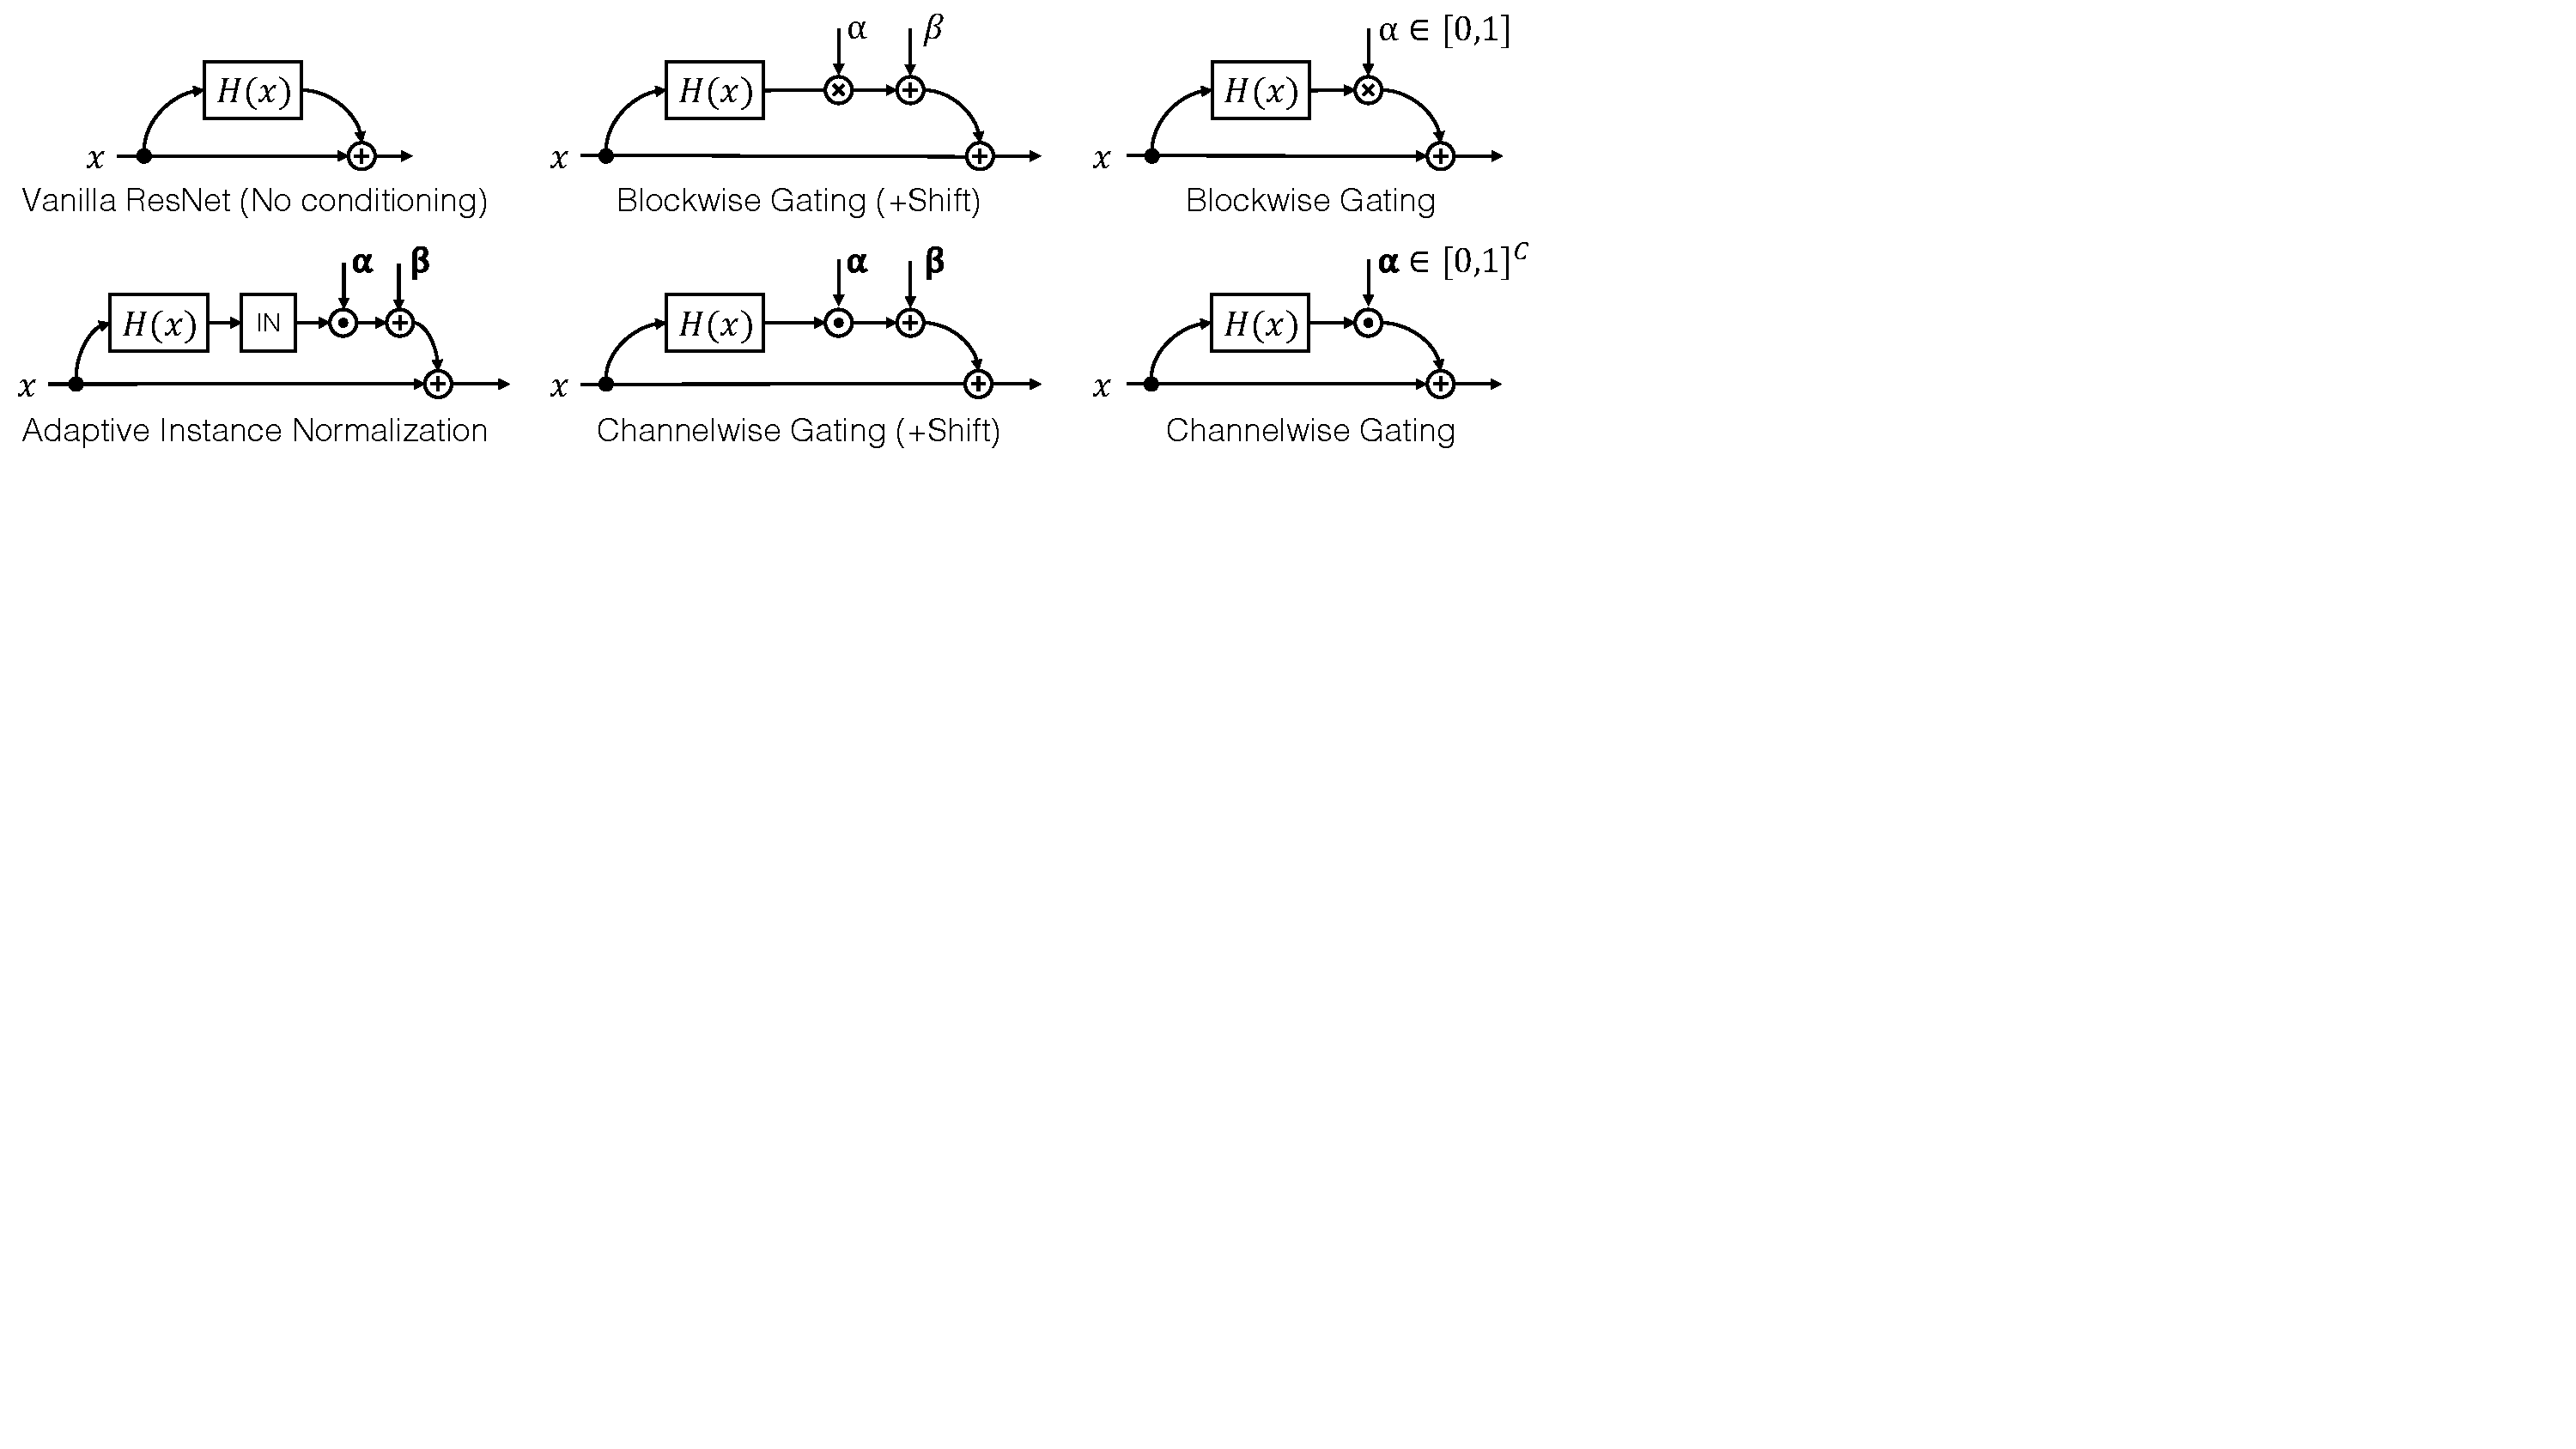
\includegraphics[width=\linewidth]{paper_images/arch_gate.pdf}
%     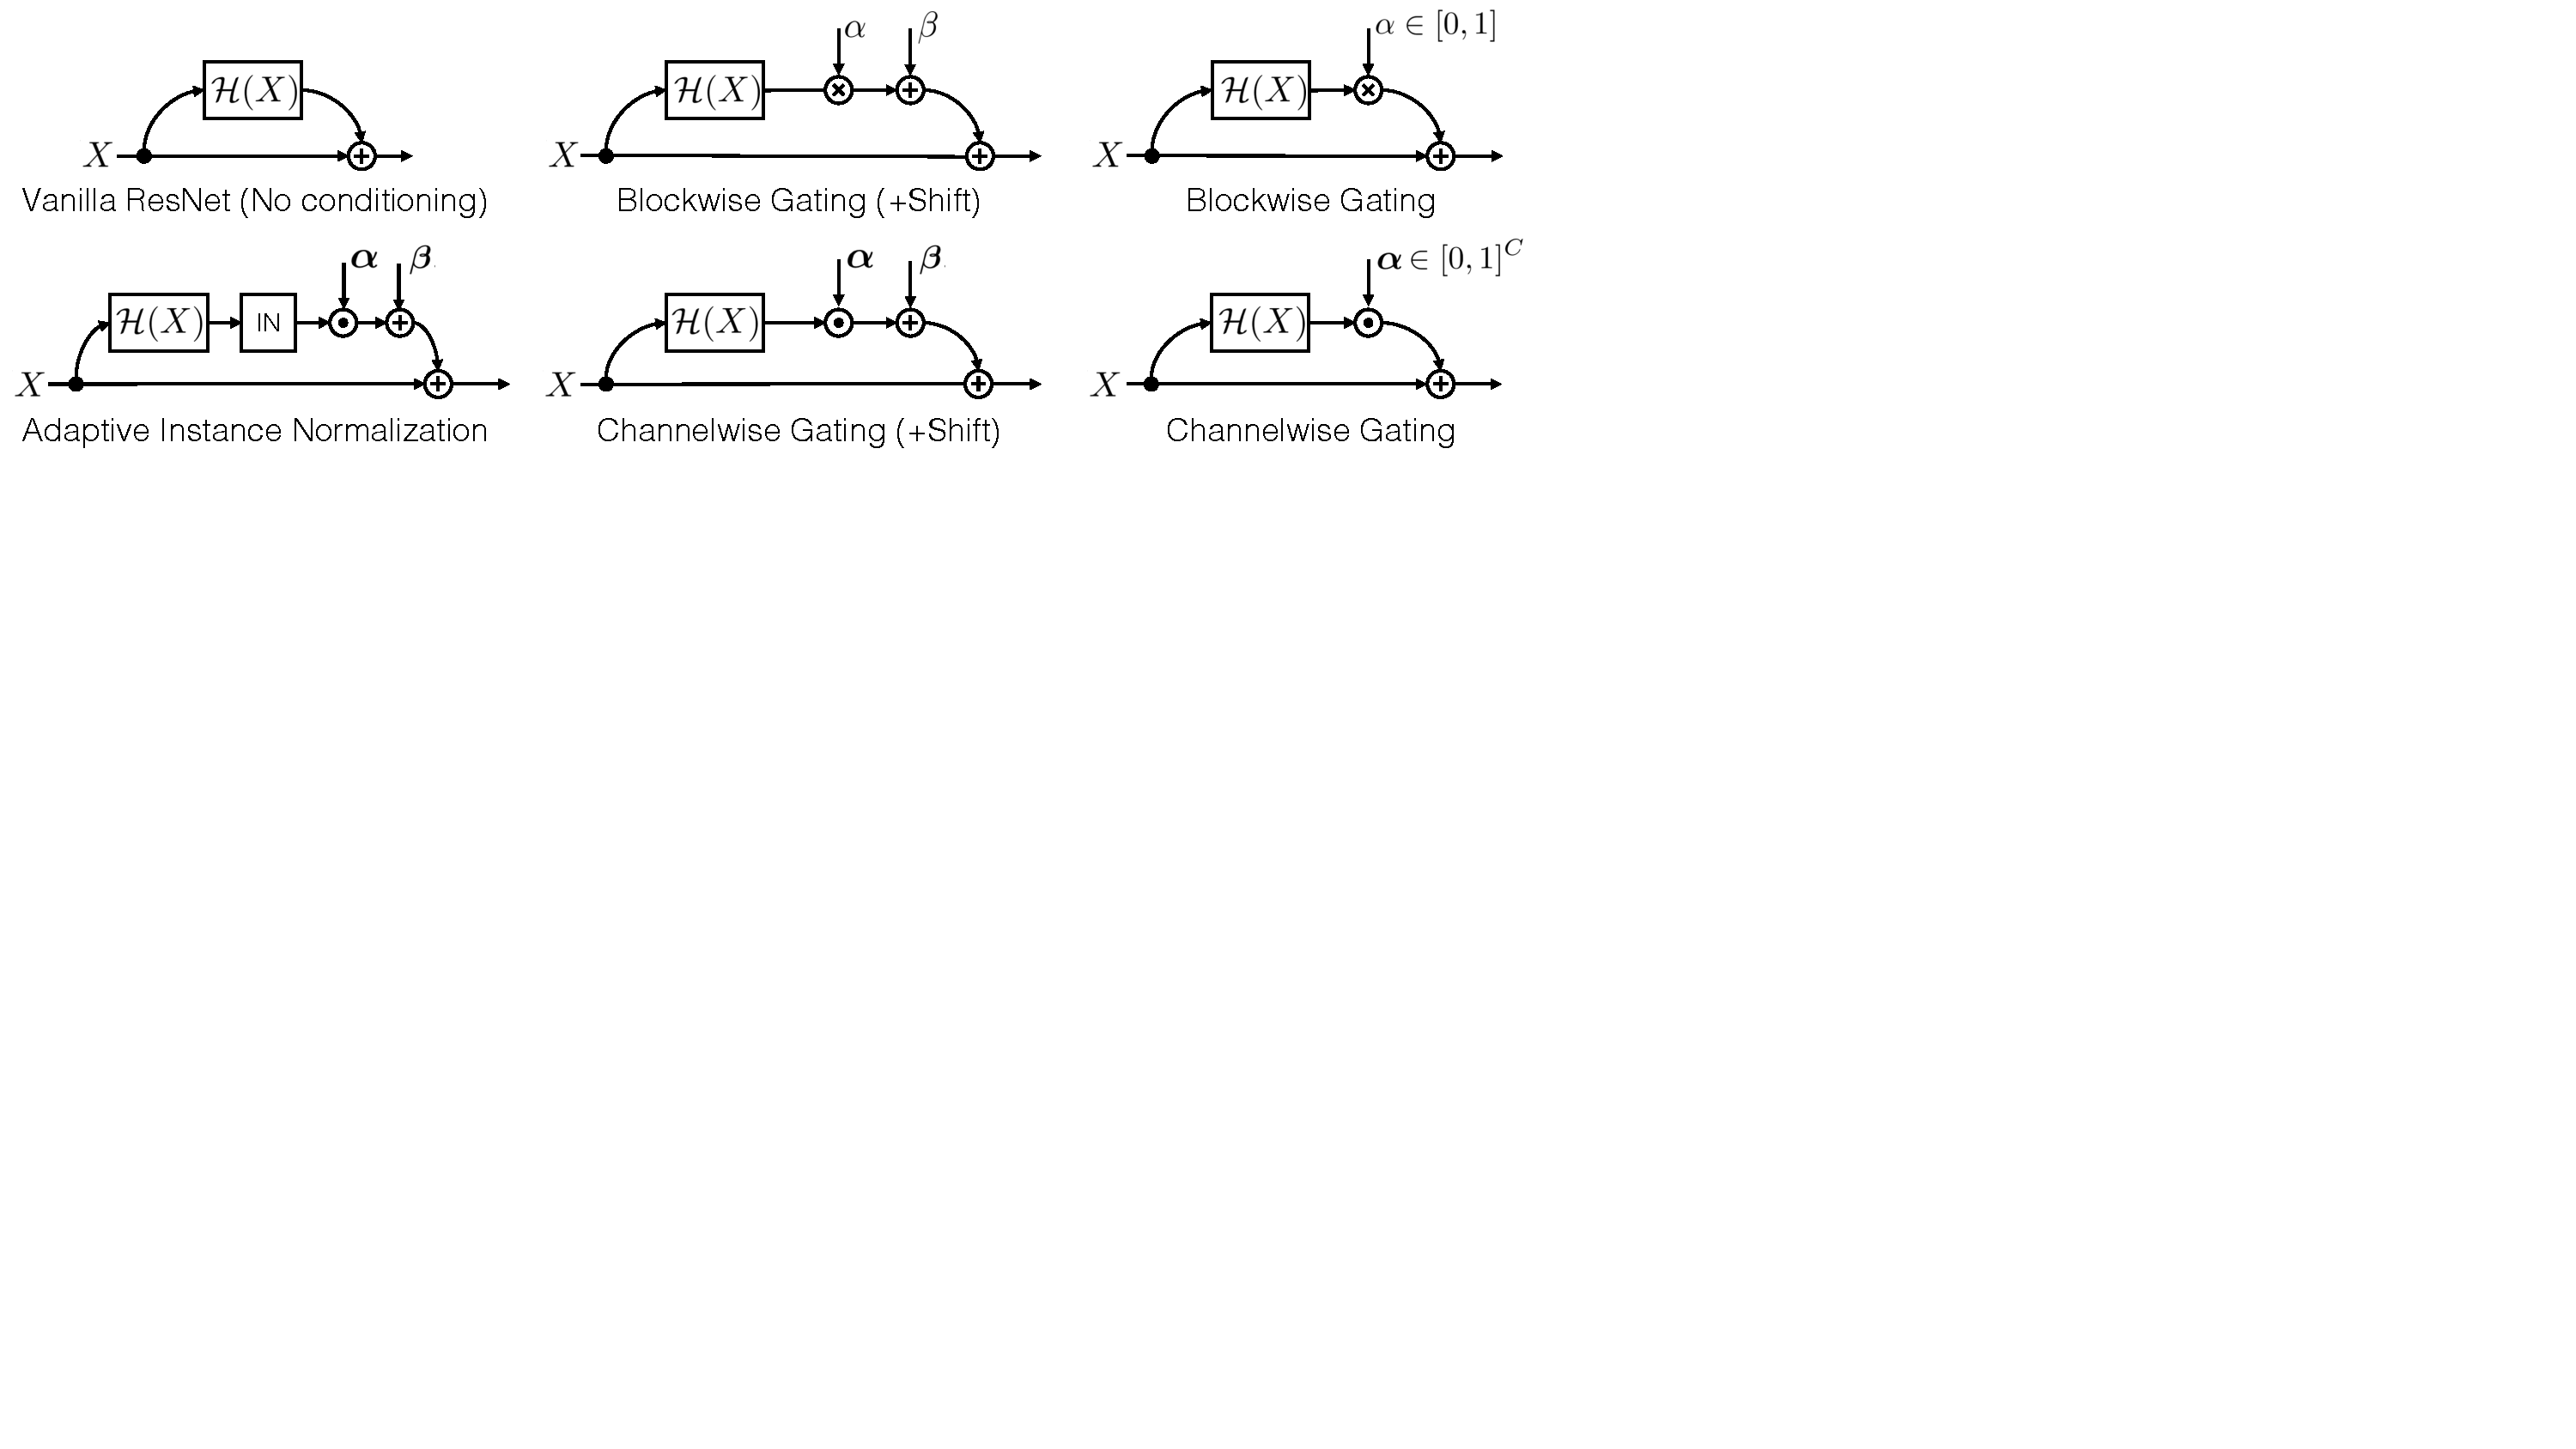
\includegraphics[width=.9\linewidth]{paper_images/arch_gate2.pdf}
%     \caption{
%     % {\bf Incorporating soft-gating into residual blocks.} \rz{Order got changed, may or may not need to add key for hadamard product}
%     {\bf (Top-left)} A ``vanilla" residual block without gated conditioning parameters modifies input tensor $X$ into $X+\mathcal{H}(X)$. Conditioning with concatenation uses this setup. {\bf (Top-mid)} The $\mathcal{H}(X)$ block is softly-gated by scalar parameter $\alpha$ and shift $\beta$. {\bf (Top-right)} Only the gating is used, without bias. {\bf (Bot-left)} Adaptive Instance Normalization~\cite{huang2017arbitrary} applies a channel-wise scaling and shifting after an instance normalization layer. {\bf (Bot-mid)} Channel-wise gating adds restrictions to the range of $\mbox{\boldmath $\alpha$}$. {\bf (Bot-right)} We find that channel-wise gating (without added bias) to empirically produce the best results.\label{fig:arch-gate}
%     \vspace{-2mm}
%     }
%     % \vspace{-4mm}
% \end{figure*}


% \begin{figure*}[t]
%     \centering  
%     \begin{tabular}{cc}
%     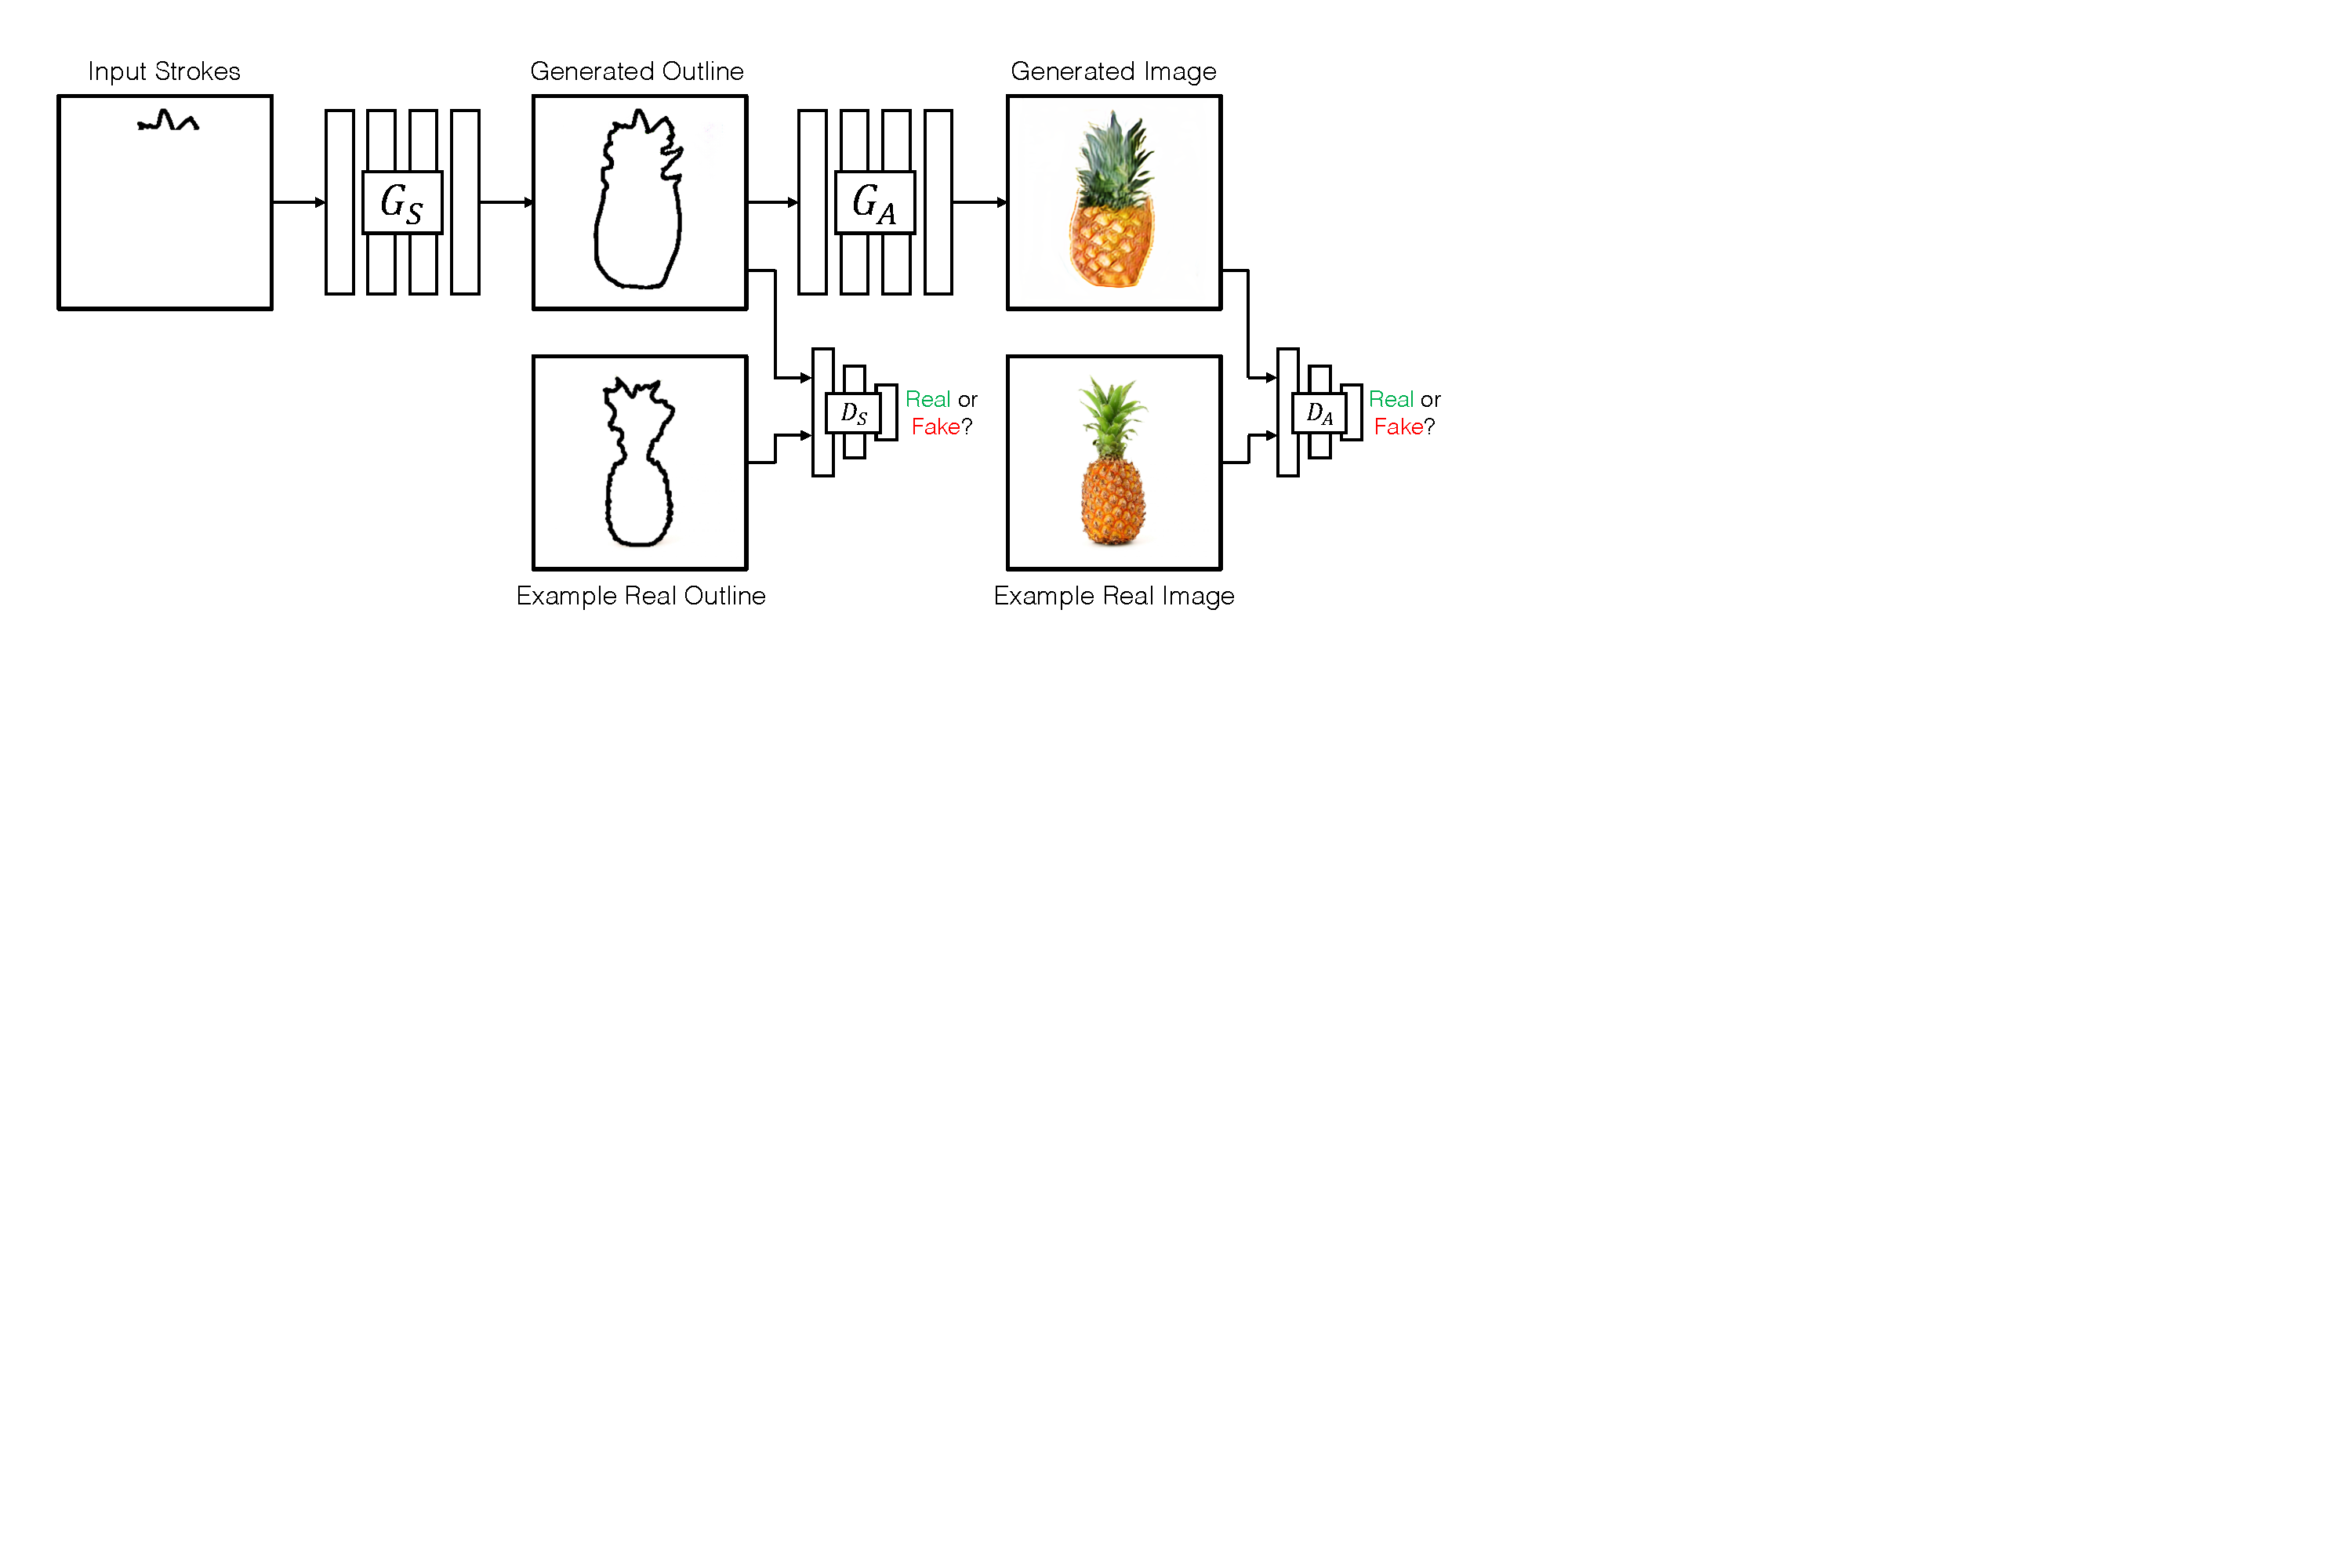
\includegraphics[width=.45\linewidth]{paper_images/isf_method_v3.pdf} &
%     \animategraphics[autoplay,loop,width=.45\linewidth]{25}{images/gif/}{00001}{00266}
%     \\
%     (a) & (b) \\
%     \end{tabular}
%         \caption{{\bf Our two-stage approach (a)} First, we complete a sketch, using the shape generator $G_S$. The appearance generator $G_A$ then translates the result into an image. Both generators are trained with respective discriminators $D_S$, $D_A$.
%         {\textbf{Video of our interface (b).} Please view with Acrobat Reader.}}\label{fig:SketchFillNet}
%         %\label{fig:gui}}
% \end{figure*}


% \begin{figure*}[t]
%     \centering  
%     \begin{tabular}{cc}
%     %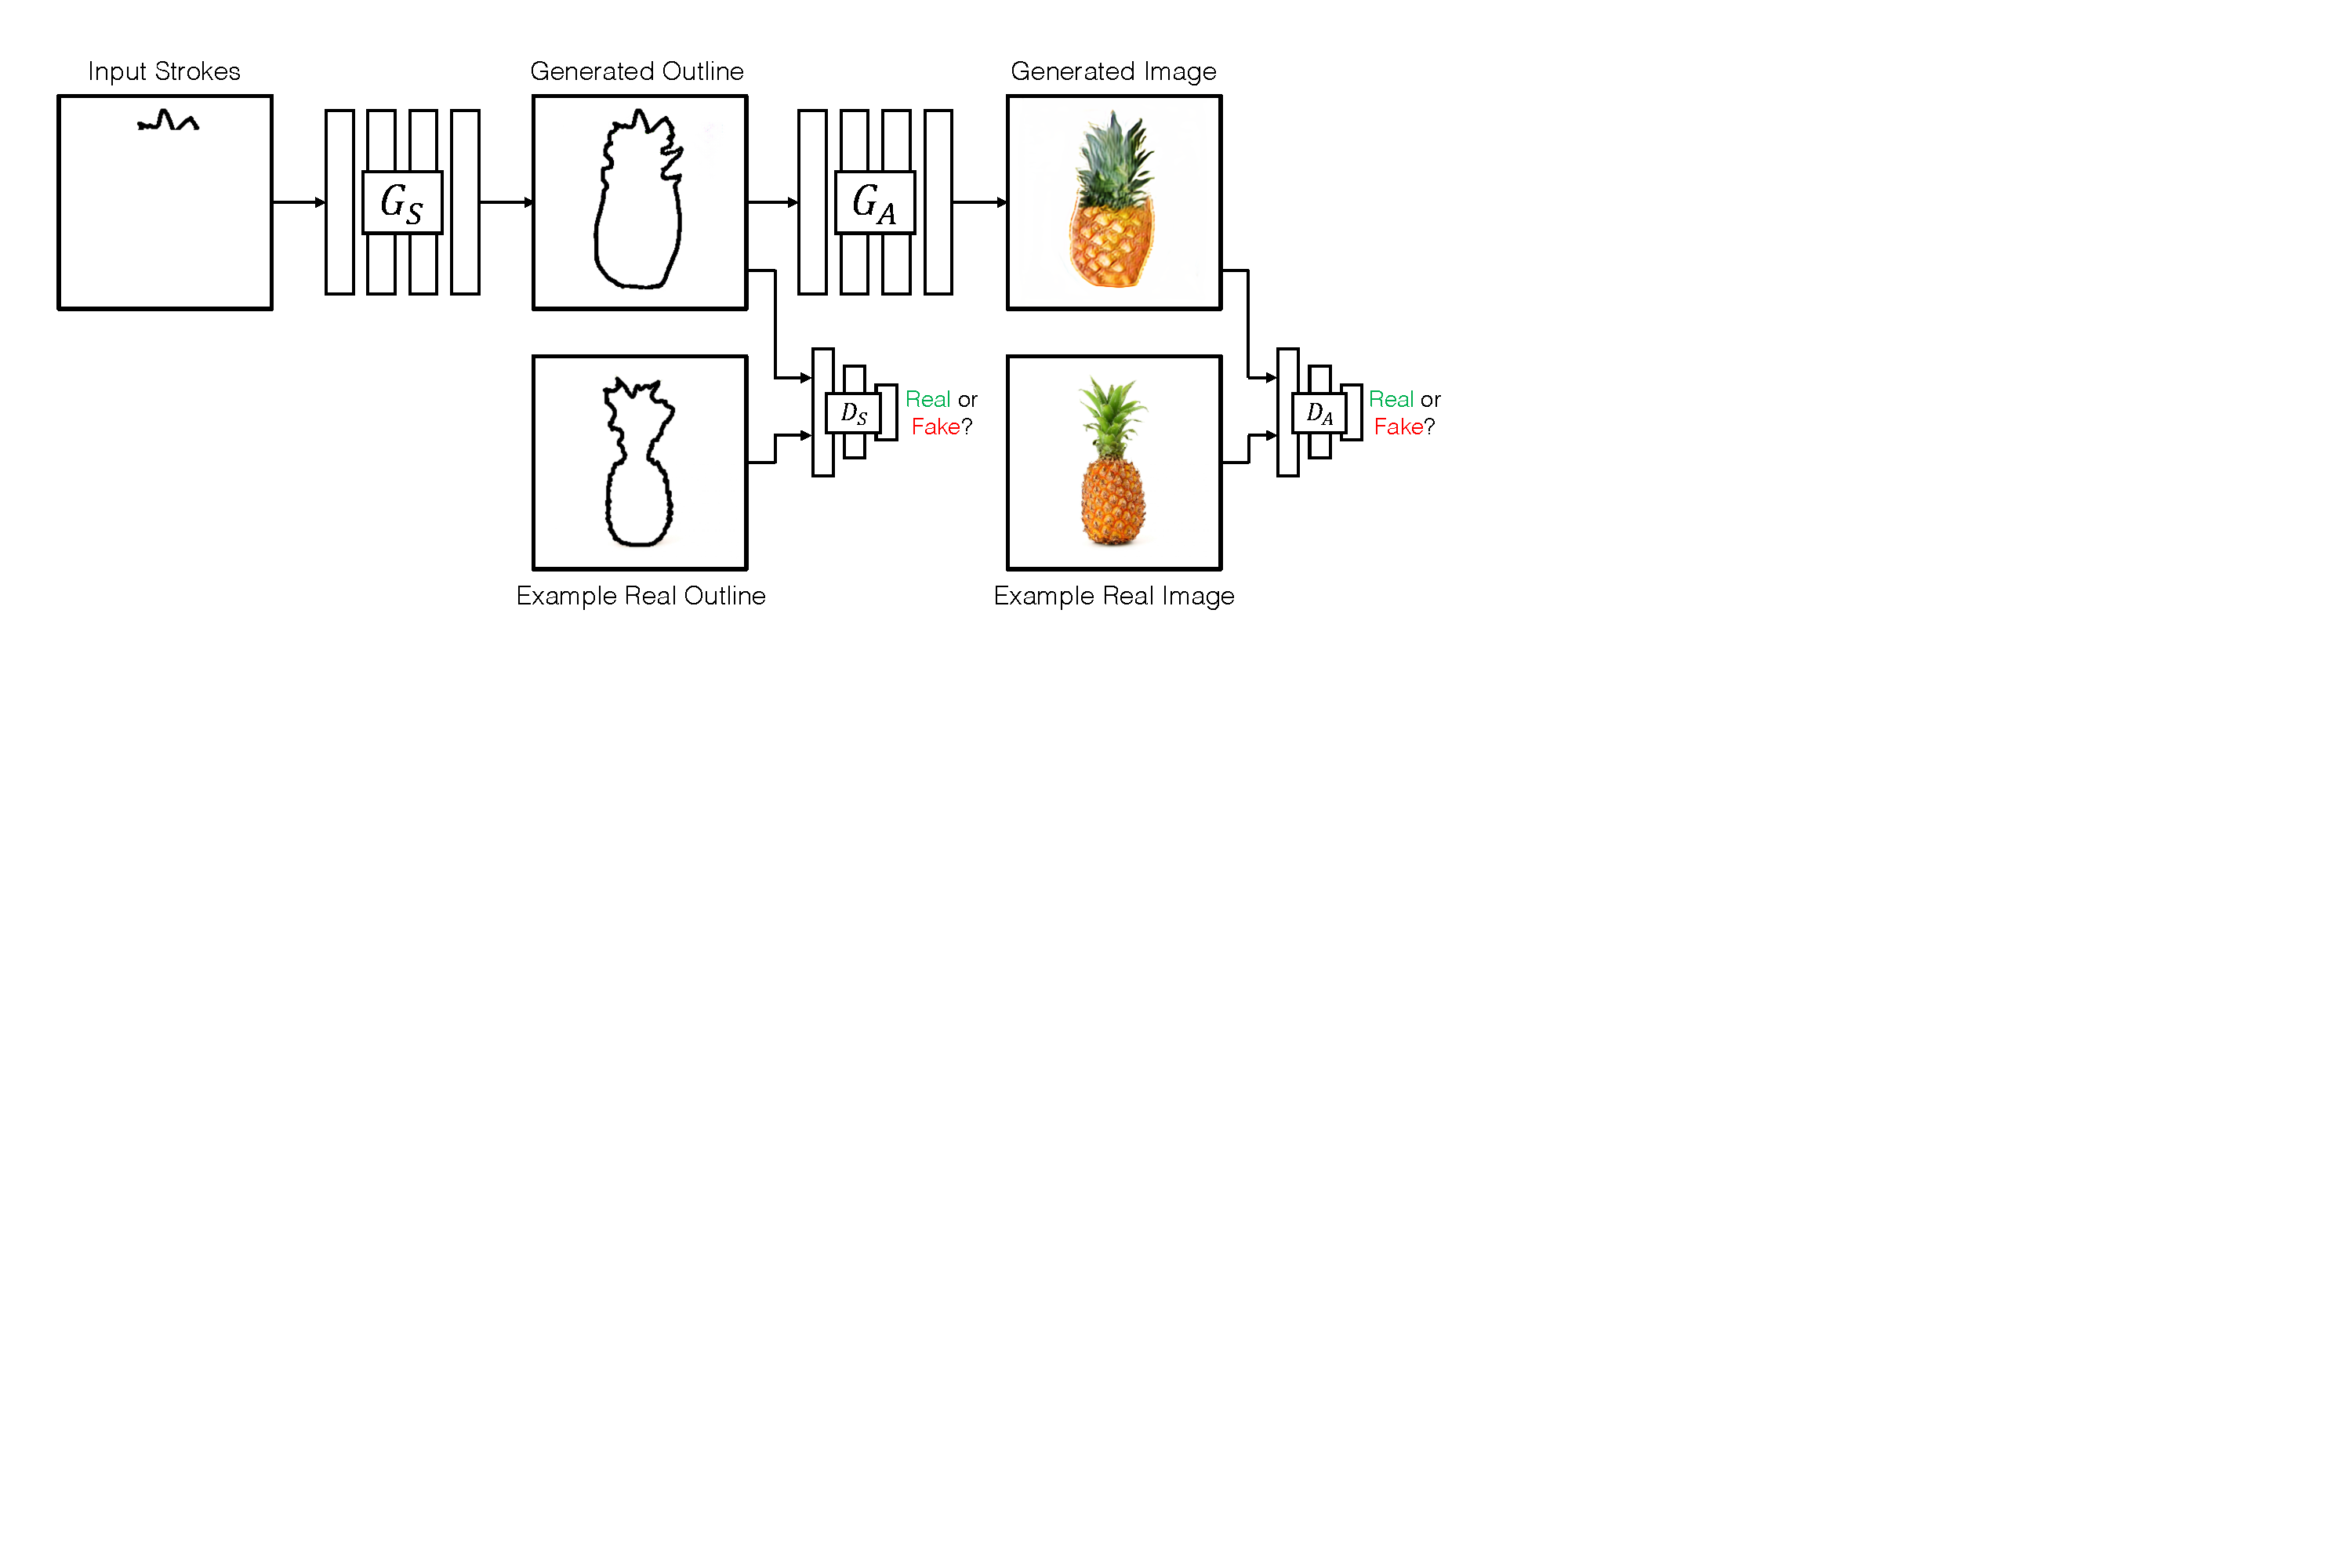
\includegraphics[width=.45\linewidth]{paper_images/isf_method_v3.pdf} &
%     \animategraphics[autoplay,loop,width=.45\linewidth]{25}{images/gif/}{00001}{00266} \hspace{4pt}
%     \animategraphics[autoplay,loop,width=.50\linewidth]{25}{images/gif_shadow/}{00001}{00419}
%     \\
%     % (a) & (b) \\
%     \end{tabular}
%         \caption{{\bf Video of our interface} We can see two versions of our interface. The left side shows how a user can quickly generate multiple objects using a few strokes, while the right side shows the utility of multimodal completions where the user can quickly explore different possible shape generations while drawing.
%         { \textbf{Please view with Acrobat Reader.}}}\label{fig:gui}
%         %\label{fig:gui}}
% \end{figure*}

\begin{figure*}[t]
    \centering  
    \begin{tabular}{cc}
    %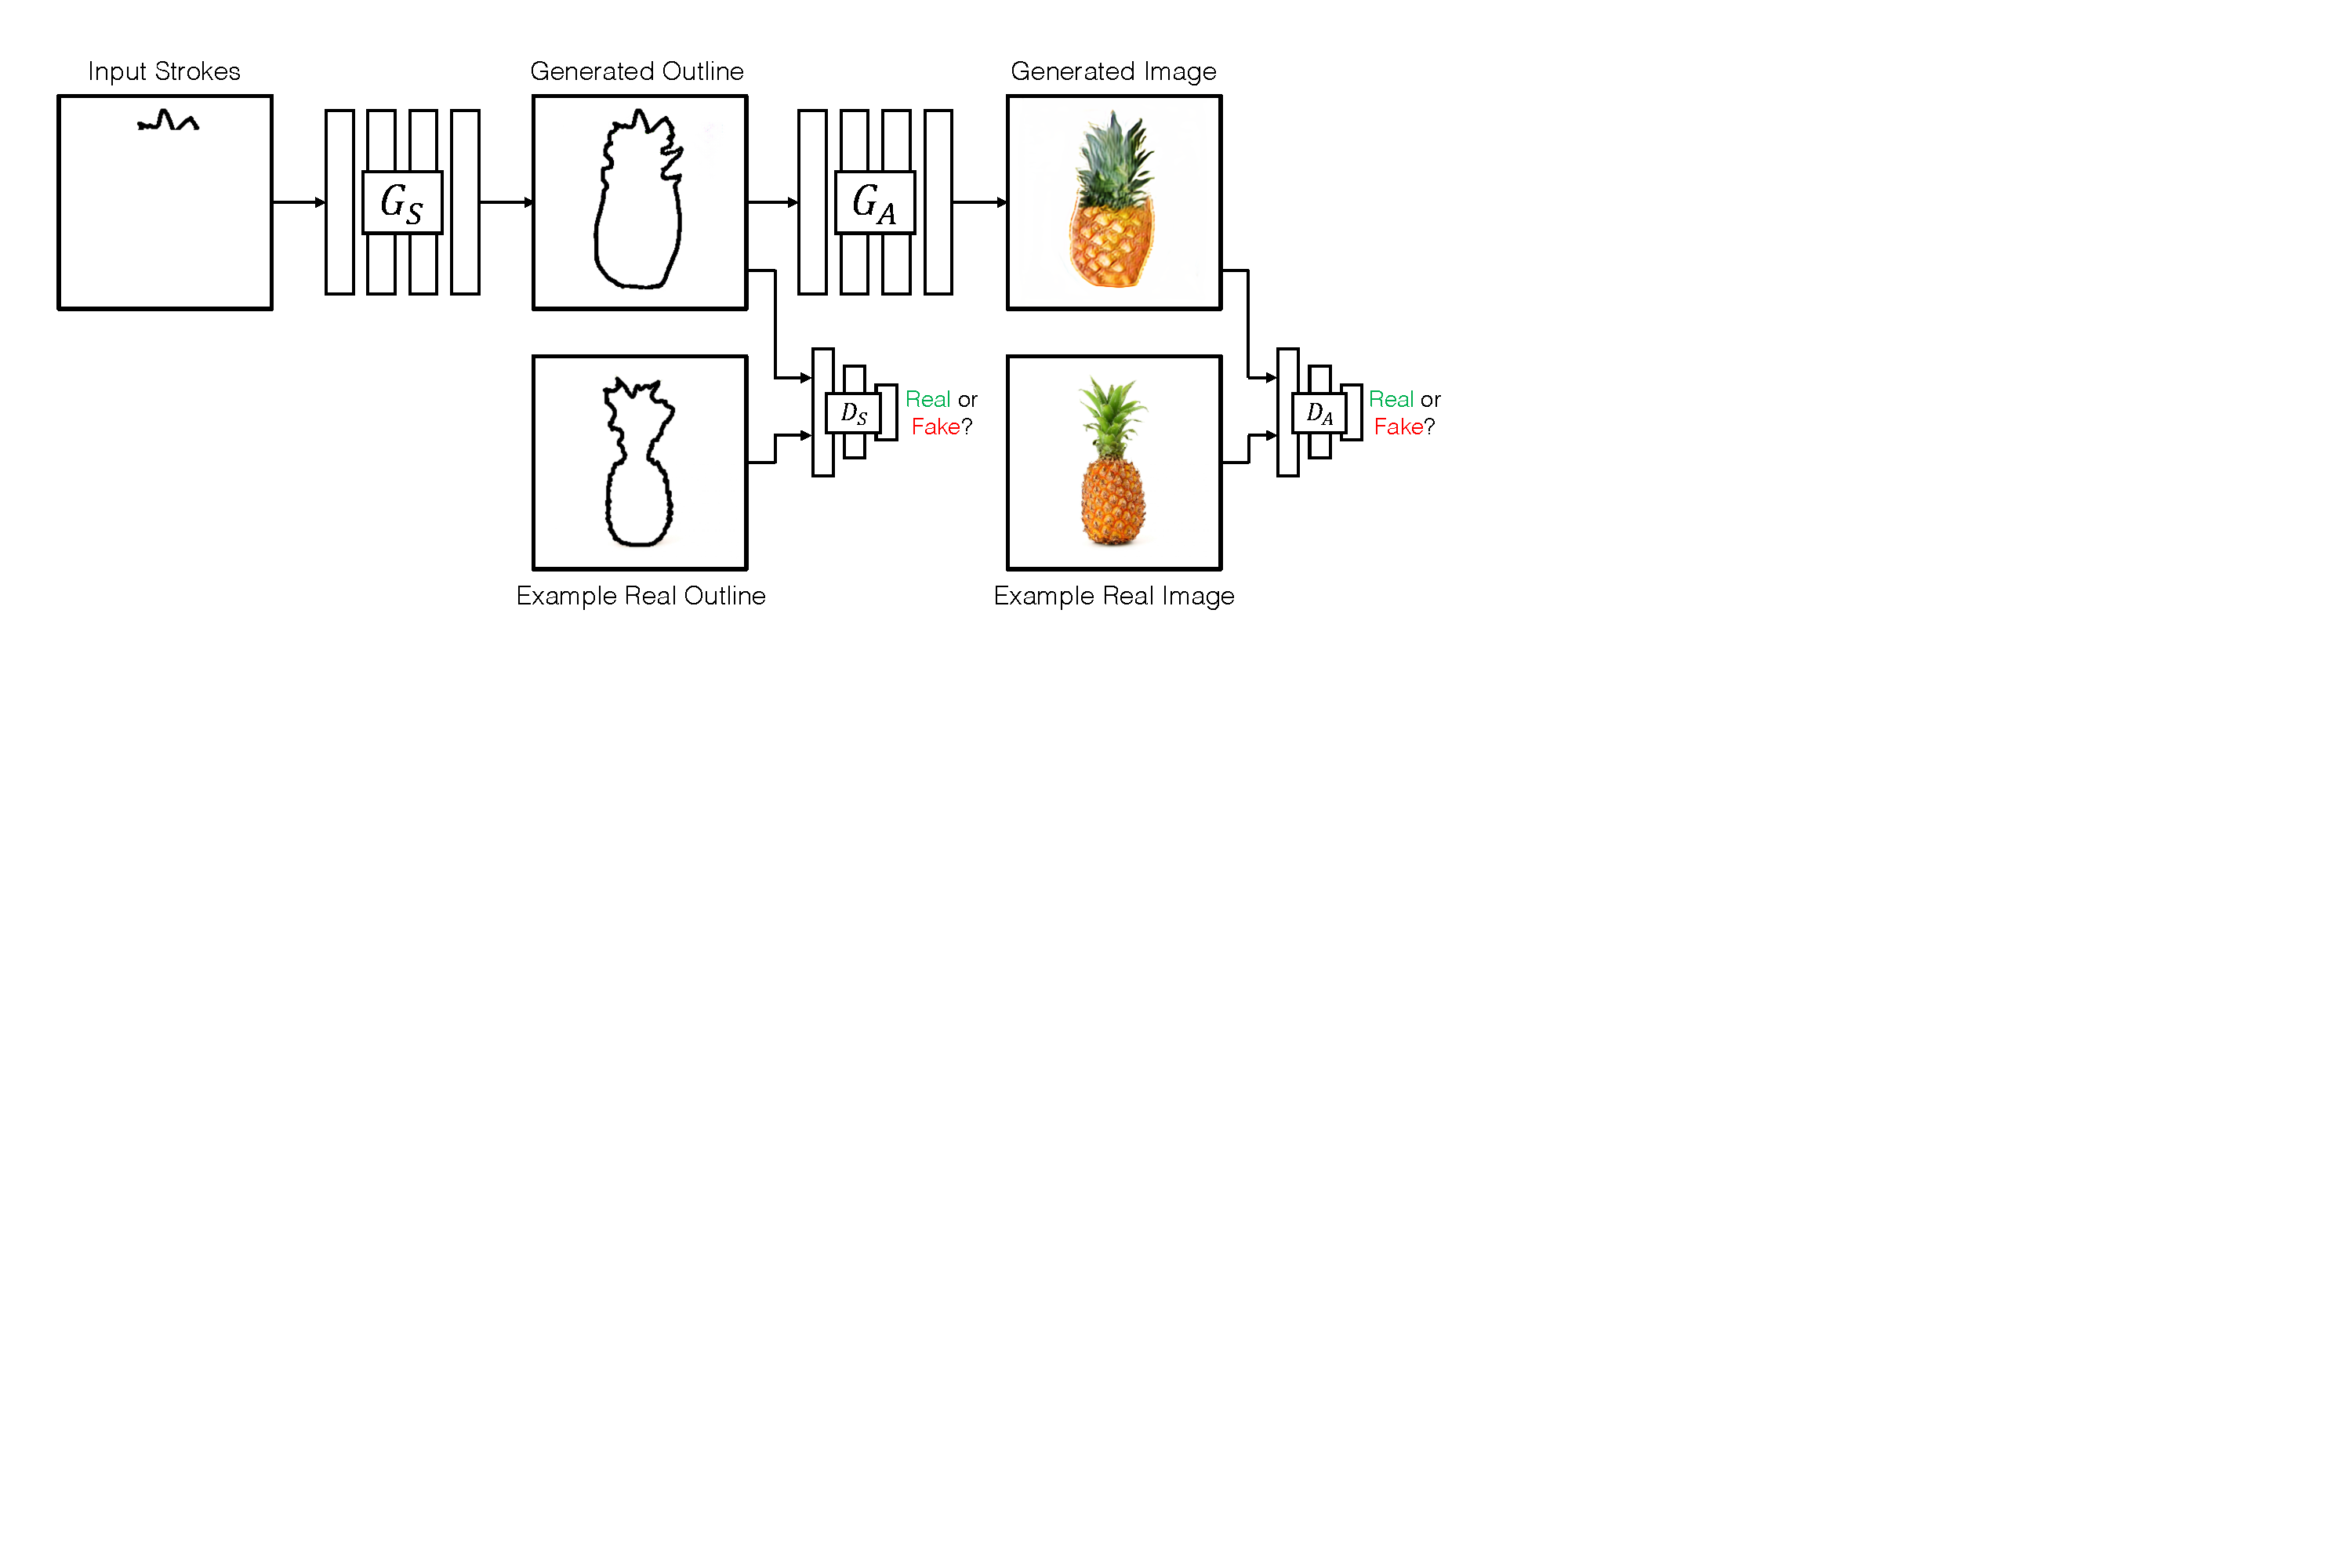
\includegraphics[width=.45\linewidth]{paper_images/isf_method_v3.pdf} &
    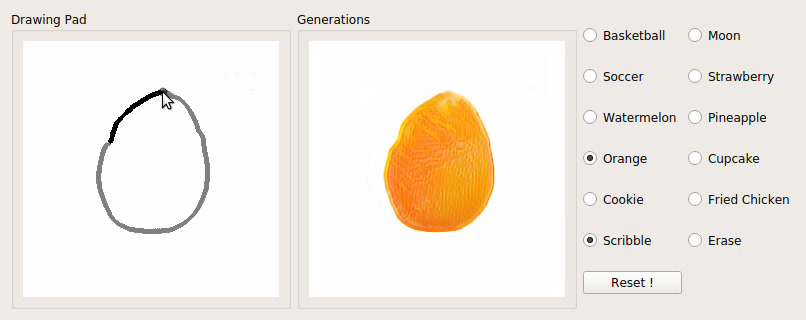
\includegraphics[width=.45\linewidth]{images/gif/00001.jpg} \hspace{4pt}
    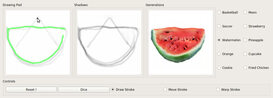
\includegraphics[width=.45\linewidth]{images/gif_shadow/00001.jpg} 
    
    \\
    % (a) & (b) \\
    \end{tabular}
        \caption{{\bf Video of our interface} We can see two versions of our interface. The left side shows how a user can quickly generate multiple objects using a few strokes, while the right side shows the utility of multimodal completions where the user can quickly explore different possible shape generations while drawing.
        { \textbf{Please view with Acrobat Reader.}}}\label{fig:gui}
        %\label{fig:gui}}
\end{figure*}


\section{Related Work}

\paragraph{Interactive Generation} Interactive interfaces for freehand drawing go all the way back to Ivan Sutherland's Sketchpad~\cite{sutherland64}.  The pre-deep work most related to us, ShadowDraw~\cite{lee2011shadowdraw}, introduced the concept of generating multiple shadows for novice users to be able to draw sketches. PhotoSketcher \cite{eitz2011photosketcher} introduces a retrieval based method for obtaining real images from sketches. %Hays et al.~\cite{hays2007scene} introduce a retrieval-based method for filling scenes.
% \es{other old papers? Talk about ShadowDraw and other non-deep methods}. 
More recently, deep recurrent networks have been used to generate sketches~\cite{ha2017neural,ganin2018synthesizing}. Sketch-RNN~\cite{ha2017neural} provides a completion of partial strokes, with the advantage of intermediate stroke information via the Quickdraw dataset at training time. SPIRAL \cite{ganin2018synthesizing} learns to generate digits and faces using a reinforcement learning approach.
% to generate programs for synthesizing the final image.
Zhu et al.~\cite{zhu2016generative} train a generative model, and an optimization-based interface to generate possible images, given color or edge constraints. The technique is limited to a single class and does not propose a recommendation for the completion of the shape. SketchyGAN~\cite{chen2018sketchygan} also aimed at generating multi-class images but lacks interactive capability. In contrast to the above, our method provides interactive prediction of the shape and appearance to the user and supports multiple object classes.
\vspace{-6mm}
\paragraph{Generative Modeling} Parametric modeling of an image distribution is a challenging problem. Classic approaches include autoencoders~\cite{hinton2006reducing,vincent2008extracting} and Boltzmann machines~\cite{smolensky1986information}. More modern approaches include autoregressive models~\cite{efros1999texture,van2016conditional}, variational autoencoders (VAEs)~\cite{kingma2013auto}, and generative adversarial networks (GANs). GANs and VAEs both learn mappings from a low-dimensional ``latent" code, sampled stochastically, to a high-dimensional image through a feedforward pass of a network. GANs have been successful recently~\cite{denton2015deep,radford2015unsupervised,arjovsky2017wgan}, and hybrid models feature both a learned mapping from image to latent space as well as adversarial training~\cite{donahue2016adversarial,dumoulin2016adversarially,larsen2016vaegan,chen2016infogan}.

\vspace{2mm} \noindent \textbf{Conditioned Image Generation} The methods described above can be conditioned, either by a low-dimensional vector (such as an object class, or noise vector), a high-dimensional image, or both. Isola et al.~\cite{isola2016image2image} propose ``pix2pix", establishing the general usefulness of conditional GANs for image-to-image translation tasks. However, they discover that obtaining multimodality by injecting a random noise vector is difficult, a result corroborated in~\cite{mathieu2015deep,pathak2016context,zhu2017toward}.
% introduced a set of tasks whereby the pixels of the input in a different domain corresponded to the pixels of the generated image.
% As a result, image-to-image translation methods have exploded in popularity, as many applications can be expressed in this framework.
% However, one problem with the original Pix2pix formulation is that the quality degrades quickly with increased class diversity. 
% We build upon these ideas by proposing a new architecture and gating scheme that allows for high quality multiclass image generation. 
% \paragraph{Mode Collapse}
This is an example of mode collapse~\cite{goodfellow2016nips}, a phenomenon especially prevalent in image-to-image GANs, as the generator tends or ignore the low-dimensional latent code in favor of the high-dimensional image.
% This is an example of mode collapse is a major challenge for GANs~\cite{goodfellow2016nips}, where the diversity of the generated results is limited and only a portion of the training set is utilized. 
Proposed solutions include layers which better condition the optimization, such as Spectral Normalization~\cite{zhang2018self,miyato2018spectral}, modifications to the loss function, such as WGAN~\cite{arjovsky2017wasserstein,gulrajani2017improved} or optimization procedure~\cite{heusel2017gans}, or modeling proposals, such as MAD-GAN~\cite{ghosh2017multi} and MUNIT~\cite{huang2018multimodal}. 
% Several techniques deal with this issue, the best performing among those include Spectral Normalization \cite{zhang2018self,miyato2018spectral} which normalizes the spectral norms of the layers to stabilize training, MAD-GAN \cite{ghosh2017multi} which introduces multiple generators, BicycleGAN \cite{zhu2017toward} which reconstructs the latent code from the generation using two cycles, and MUNIT \cite{huang2018multimodal} which introduces a factorized latent space for content and style for producing variations.
One modeling approach is to add a predictor from the output to the conditioner, to discourage the model from ignoring the conditioner. This has been explored in the classification setting in Auxiliary-Classifier GAN (ACGAN)~\cite{odena2016conditional} and regression setting with InfoGAN~\cite{chen2016infogan} and ALI/BiGAN (``latent regressor" model)~\cite{dumoulin2016adversarially,donahue2016adversarial}, and is one half of BicycleGAN model~\cite{zhu2017toward}. We explore a complementary approach of architectural modification via gating.

% \ow{not clear to me why it starts with mode collapse... dangerous as we also have it in our results, except the infogan case. I think that this should be changed into an infogan related work section and moved below.}

%but needed far more details such as in the case of edge to handbags generation task it needed texture strokes inside the bag as well to be able to produce high quality diverse generations
%Other forms of conditioning have been introduced in \cite{wang2018video} whereby rough triangles and sparse edges are enough to generate high quality videos. We explore the situation in which the input scribble is extremely sparse and multiple classes can have very similar input scribbles for instance in the case of balls the input scribble is just the outline in the shape of a circle.

%Our architecture also differs from previous art in the form of the architecture whereby all the blocks are residual including the downsampling and upsampling. Previous literature mostly used the residual blocks in the bottleneck layer of an Encoder Decoder structure. The number of channels in the networks doesn't change with the change of resolution as in the original Resnet architecture \cite{he2016deep} in order to ease the learning of the gating mechanism. 

\vspace{2mm} \noindent \textbf{Gating Mechanisms}
%Residual Networks \cite{he2016deep} introduced a new set of architectures that enabled training of very deep networks.
Residual networks~\cite{he2016deep}, first introduced for image classification~\cite{krizhevsky2012imagenet}, have made extremely deep networks viable to train. Veit et al.~\cite{veit2016residual} find that the skip connection in the architecture enables test-time removal of blocks. Follow-up work~\cite{veit2018adaptive} builds in block removal during training time, with the goal of subsets of blocks specializing to different categories. Inspired by these results, we propose the use of gating for image generation and provide a systematic analysis of gating mechanisms.
% Prior work has demonstrated that in ResNets, some paths are more important for particular classes~\cite{veit2016residual}, and has used this to develop a hard gating mechanism~\cite{veit2018adaptive}.
% We provide a further analysis of gating mechanisms, in the context of GAN image generation, as opposed to image classification.

The adaptive instance normalization (AdaIn) layer has similarly been used in arbitrary style transfer~\cite{huang2017arbitrary} and image-to-image translation~\cite{huang2018multimodal}, and Feature-wise Linear Modulation (FiLM)~\cite{perez2017film}. Both methods scale and shift feature distributions, based on a high-dimensional conditioner, such as an image or natural language question. Gating also plays an important role in sequential models for natural language processing: LSTMs \cite{hochreiter1997long} and GRU \cite{cho2014learning}. Similarly, concurrent work \cite{karras2018style}, \cite{park2019semantic} use a AdaIN-style network to modulate the generator parameters.
% \es{Mention concurrent work? StyleGAN, Taesung's paper}

% Our approach is related to adaptive instance normalization (AdaIn) has been used to great success in style transfer~\cite{huang2017arbitrary} and multimodal image-to-image translation~\cite{huang2018multimodal}.
% We use a fully residual architecture, and employ soft-gating both in the generator and discriminator. 
%Although previous work has explored the idea of gating via AdaIN in the generator but our techniques also involves using gating in the discriminator as well. 
% We evaluate AdaIn style gating among other possible choices with our architecture, and show that channel gating achieves superior performance for our task. Another gating mechanism, FiLM~\cite{perez2017film}, was introduced in the context of Visual Question Answering.
% In this case, the gating mechanism is conditioned on the input question.
% Gating also plays an important role in natural language processing: LSTMs \cite{hochreiter1997long} and GRU \cite{cho2014learning}.


% The seminal work by \cite{miyato2018spectral}, introduced spectral normalization which normalizes the weights of the network such that the maximum eigen value of the resulting set of weights is bounded. It helped enormously in stabilizing the training of GANs and albeit they only applied spectral normalization to the discriminator, SA-GAN \cite{zhang2018self} applied it to both the generator and discriminator and showed superior generative modeling performance over several tasks. SA-GAN further introduced the self attention layer based on the innovative transformer network and showed not only better geometric properties being modeled by the GAN but also allowing Multi-Class generations.
% The Projection Discriminator \cite{miyato2018cgans} based Conditional GANs altered the naive model of concatenating the condition provided to the discriminator via a generalized bilinear projection between the condition and the features extracted from the image thereby providing more finegrained gradients suitable for training the generator to produce class conditional and better resolution images. 
% MAD-GAN \cite{ghosh2017multi} introduced multiple generators and showed an innovative experiment whereby they mixed images from 3 classes and the 3 generators could disentangle the classes and each of the generators generated much sharper images from a particular class than a single generator with similar capacity could. 

% %moved from intro
% To combat this challenge a solution called MAD-GAN \cite{ghosh2017multi} was proposed which dealt with the issue via multiple generators whereby the discriminator distributed the modes and classes in the data distribution among the various generators. 
% Although MAD-GAN was a novel solution to deal with discontinuities in the manifold of the multi-class data distribution, the solution came with its flaws, supreme among them was the reduced scalability in the case the structure was not shared among the different classes, the generators couldn't share the initial layers' parameters and therefore was limited by GPU capacity and in practice going more than 5-6 generators was difficult. 

% In another line of papers which helped build the ideas in this paper are the research on Residual Networks \cite{he2016deep} which introduced a set of architectures which allowed extremely deep networks to be trained upto hundreds of layers which was earlier assumed to be extremely difficult because of the problem of vanishing gradients in deep networks. The residual connection allowed a unadulterated gradient backpropagation pathway which enabled training of ultra deep networks. A thorough analysis of residual networks by \cite{liao2016bridging} showed that residual networks have similar connections to unrolled recurrent neural networks without weight sharing and is very similar to how computation unfolds in human brains. Veit et al. \cite{veit2016residual} did a set of innovative incision experiments whereby they removed some blocks and allowed only the skip connection to be active in a trained Residual Network and they were able to demonstrate that even after removing some layers there a very miniscule reduction in the classification accuracy while a similar incision in a VGG network \cite{simonyan2014very} which doesn't have skip connections led to almost random outputs in the task of classification. \cite{veit2016residual} also demonstrated that residual networks behave as an ensemble of several shallower networks. \cite{veit2018adaptive} used the concepts introduced in \cite{veit2016residual} to introduce a discrete gating mechanism in deep residual networks based on the Gumbel-Softmax approximation to make the discrete decision differentiable. Their approach allowed redundant computations in the residual blocks to be reduced and to use only few of the blocks in the trained network during testing phase of the neural network. \cite{de2017modulating} introduced a technique for modulating the activations of a residual block by predicting the parameters of batch normalization which they term as Conditional Batch Normalization. In a similar vein \cite{perez2017film} also used a similar technique for modulating the activations of the various blocks conditioned on the question in a Visual Question Answering scenario.

% Gating mechanisms have generally been useful for language modeling tasks such as LSTMs \cite{Hochreiter1997LSTM} and \cite{chung2014empirical} which improved language modeling performance over vanilla RNNs. Gating also helped in the case of image recognition as demonstrated in Highway Networks \cite{srivastava2015highway} albeit it has a lot of resemblance to residual networks. 

% Image manipulation and Generation has seen huge strides in recent years with the advent of Generative Adversarial Networks \cite{goodfellow2014generative}, style transfer networks \cite{gatys2015neural} and image colorization \cite{zhang2016colorful}. iGAN \cite{zhu2016generative} was one of the first very innovative papers that introduced us to a novel technique for editing images using neural networks and preventing the edited images to fall off the natural image manifold. Pix2pix \cite{isola2016image2image} introduced a novel network based on GANs which could translate images on a plethora of datasets such as edges to handbags, semantic layout to photo realistic images and day to night. Cutting edge techniques on similar lines include \cite{wang2018video} which can translate from Video to Video such as from pose sequences to a person dancing or from semantic layouts to photorealistic road scenes. InfoGAN \cite{chen2016infogan} introduced a novel network based on GANs and Information Theoretic principles which could disentangle modes in the data distribution based on an unsupervised objective but showed poor performance in being able to disentangle modes and produce stochastic variations in the setting of pix2pix which is known to collapse to a single output for a particular input whereas ideally it should be a distribution. Bicycle GAN \cite{zhu2017toward} introduced 2 cycles which was able to produce stochastic generated outputs in the case of image to image translation. Another innovation was CycleGAN \cite{zhu2017unpaired} which allowed unpaired image to image translation as well as unpaired domain transfer which enabled several transformations which wasn't possible earlier. 



% \input{src/3_preliminary.tex}

\begin{figure}[t]
    \centering
    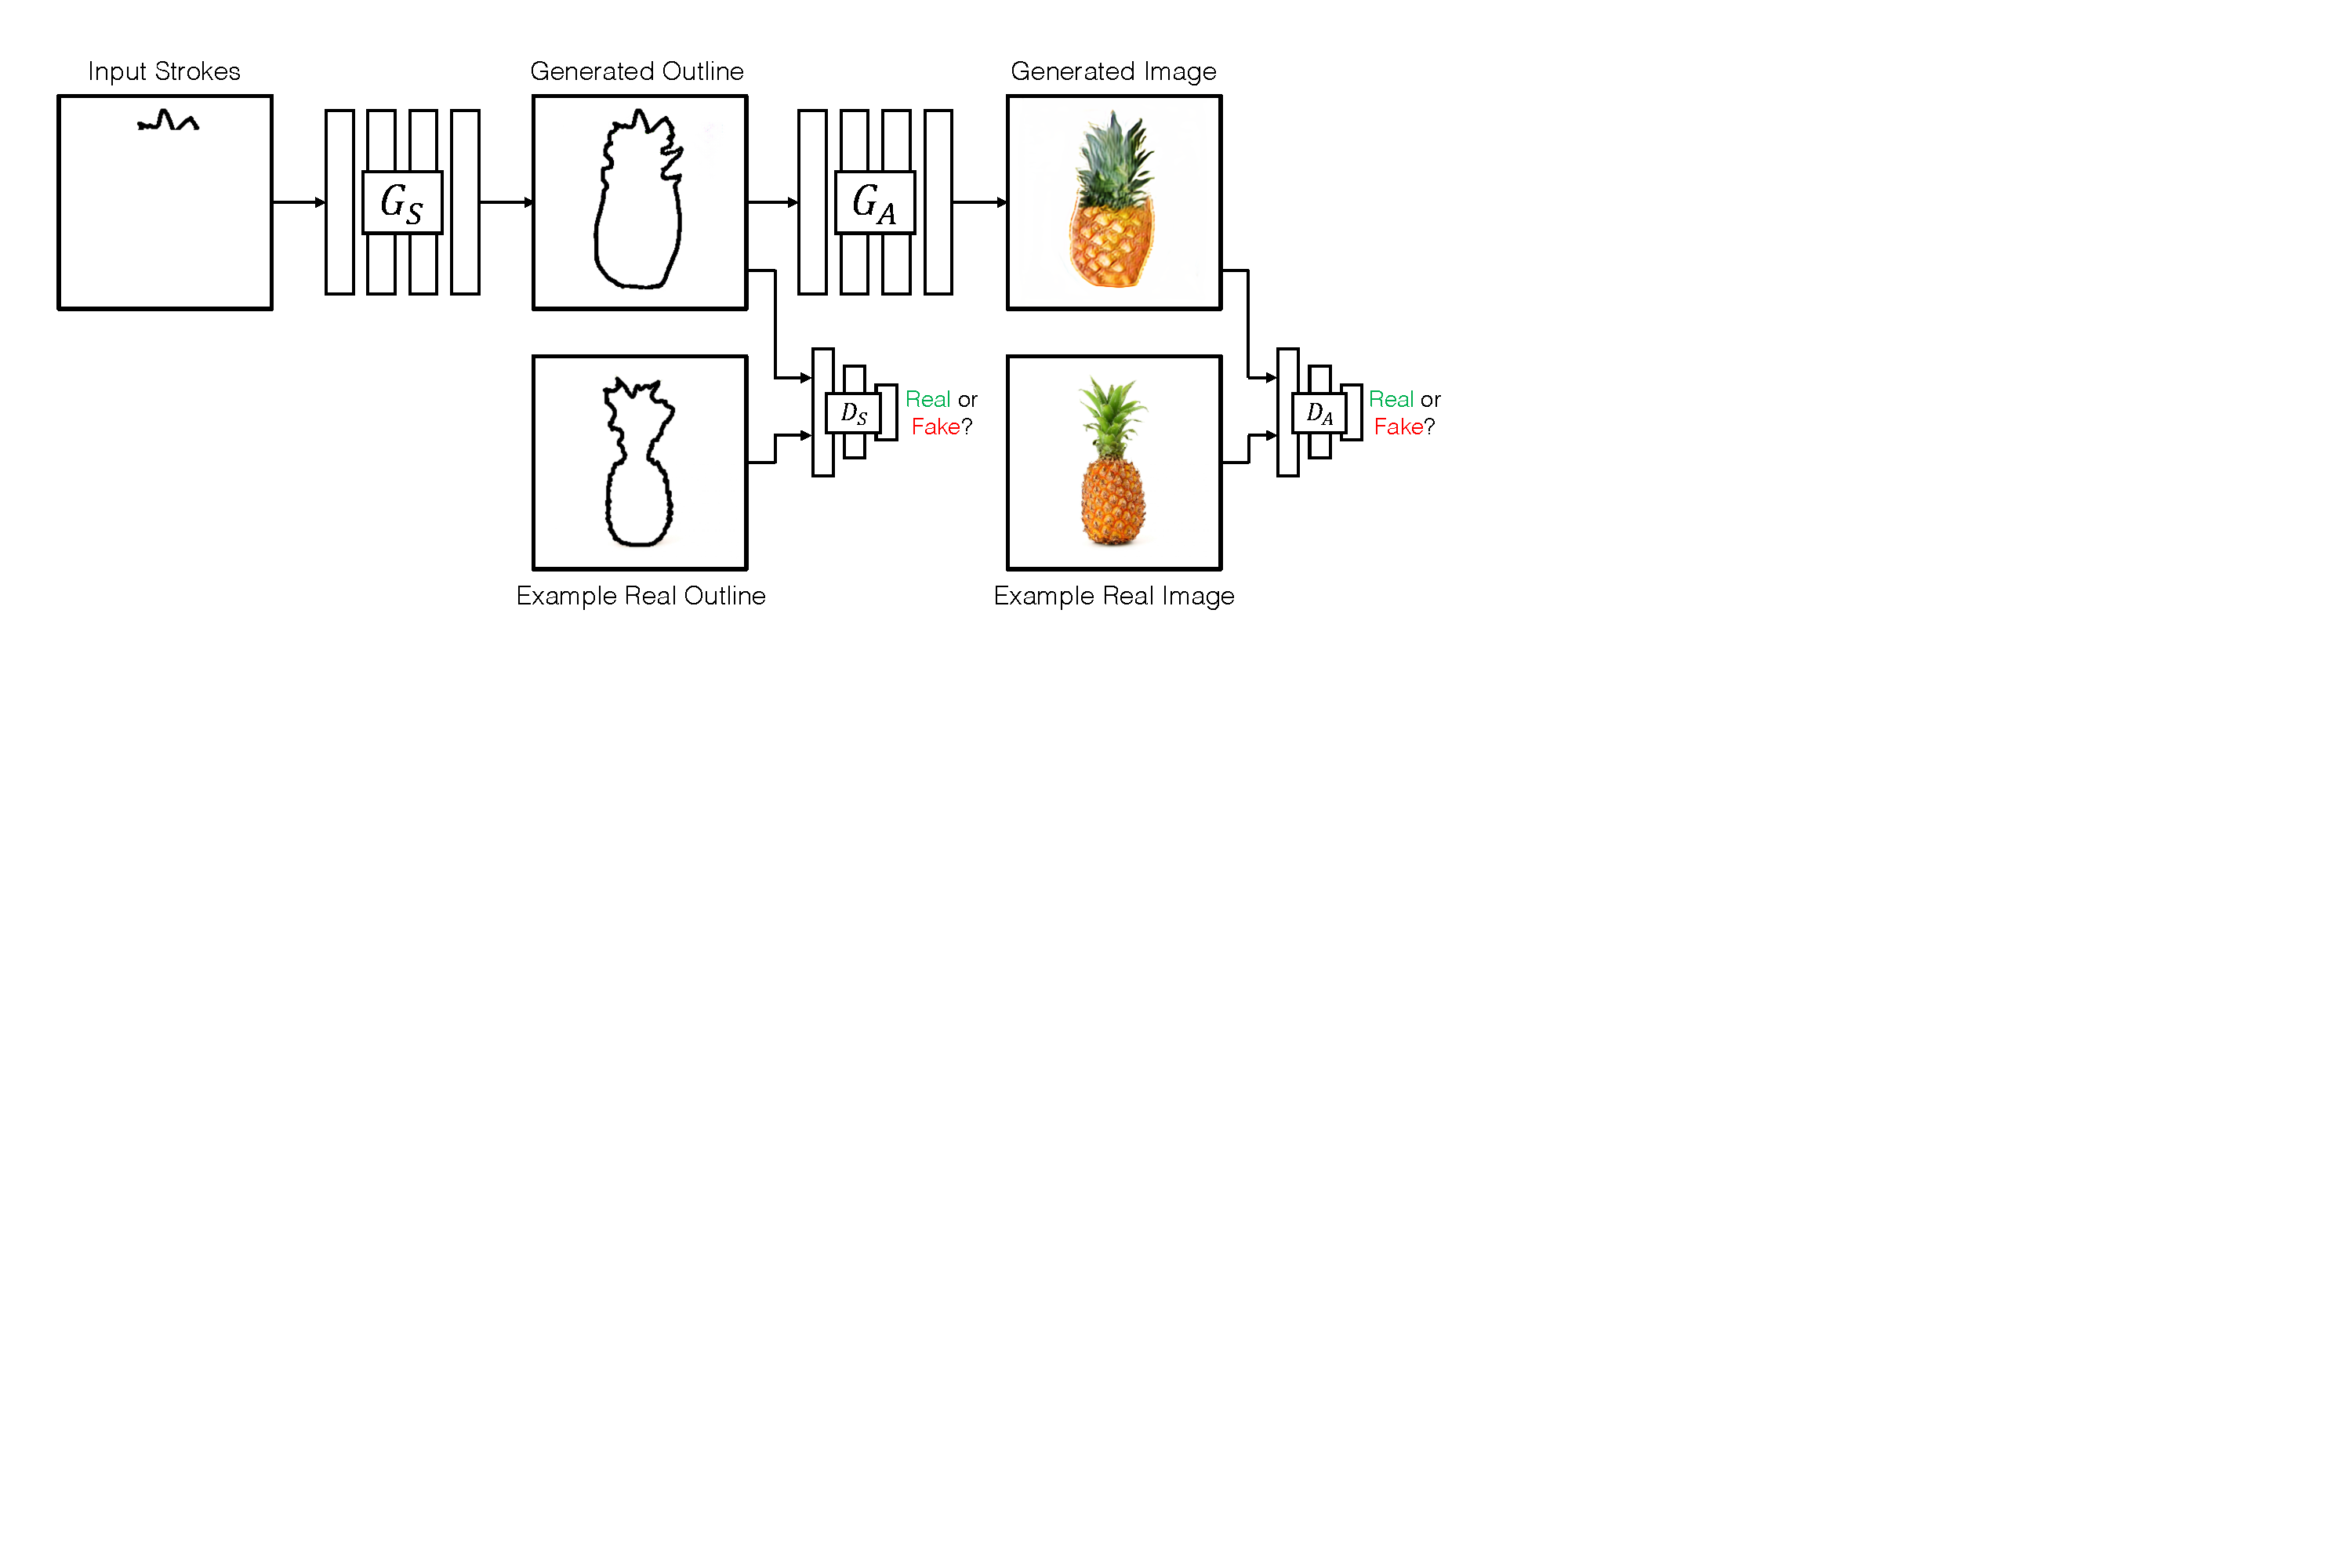
\includegraphics[width=\linewidth]{paper_images/isf_method_v3.pdf}
    \caption{Training the model to generate realistic outlines from partial strokes using $G_S$ (Shape Generator) and generating real images from outlines using $G_A$ (Appearance Generator), alongside the discriminators for the respective domains of $D_S$ (Shape Discriminator) and $D_A$ (Appearance Discriminator).
    }\label{fig:SketchFillNet}
    %\vspace{-2mm}
\end{figure}



\label{sec:methods}


% \section{Methodology (New)}
% First talk about the two inherent problems: partial (interactive) to full (task1), and outline to image (task2). mention that jointly training didn't work, analysis provided in the experiment section, so we go for two stage training. One potential reason for the joint training to fail would be that task1 requires understanding category-specific geometry and task2 requires filling the category-specific texture. Learning both jointly is difficult.

% \subsection{Interactive partial to full outline completion}
% \begin{itemize}
%     \item simple approach, data-driven, multiple partials to single full outline
%     \item used Bicycle GAN
%     \iten works surprisingly well
% \end{itemize}

% \subsection{Outline to real image synthesis}
% \begin{itemize}
%     \item Again, used GAN. objective is to train one GAN for multiple object categories
%     \item naive approach didn't work as conditioning seemed not that informative, mixed multiple categories together, bad results
%     \item used gating as it helps network to focus on the parts (or activations) of the network specific to  the features needed for a given category
%     \item just show the gating figure, explain what is means when it comes to modifying the architecure 
%     \item mention that there is information theoretic properties as well which you will discuss in the following subsection (refer)
% \end{itemize}

% \subsection{Insights on gatings}
% \begin{itemize}
%     \item put the mutual information based intuition (not sure)
%     \item mention that just to verify this, you trained infoGAN with gating on image to image and surprisingly it produced diverse generations which otherwise requires sophisticated and well thought models such as BicycleGAN, MAD-GAN etc
%     \item you can also talk about the 1D experiments here
% \end{itemize}

\section{Method}
We decouple the problem of interactive image generation into two stages: outline (or object shape) completion from sparse user sketches, and appearance synthesis from the completed outline. More specifically as illustrated in \figref{fig:SketchFillNet} we use the Shape Generator $G_S$ for the automatic shape (outline) generation and the Appearance Generator $G_A$ for generating the final image as well as the adversary discriminators $D_S$ and $D_A$. The method can be seen effective in the user interface in \figref{fig:gui}.
%To ensure that the generated shape completions and appearance completions are accurate for their respective domains we use the Shape Discriminator $D_S$ and the Appearance Discriminator $D_A$.
% \es{we need to refer to Fig.~\ref{fig:SketchFillNet} and use it's terminology $G_S$, $G_A$, ...}
%A naive method of bypassing this two step process and generating the final image from the partial strokes yielded sub-par results demonstrated in Section \ref{sec:experiments} hence necessitating the 2 step process. 
%A potential reason for the failure of the direct process is because it requires understanding category-specific geometry and the category-specific texture. Learning both jointly is difficult.

\subsection{Shape completion}
\label{sec:shape}
The shape completion network $G_S$ should provide the user with a visualization of its  completed shape, based on user input, and should keep on updating the suggested shape interactively. 
%For an interactive user interface to be effective, the network has to generate an estimated full image shape as the user adds sparse input. 
We take a data-driven approach for this whereby, to train the network, we simulate partial strokes by removing random square patches from the full outline image. 
The patches are of three sizes (64$\times$64, 128$\times$128, 192$\times$192) and are placed at a random location in the image (of size 256$\times$256). An illustration can be seen in \figref{fig:autocomplete_data_generation}.
% \es{probably need more details here - size of squares, how many per image, total training data size etc.}
We automatically generate data in this manner creating a dataset where 75 different partial outlines are created from a single outline image.
We found that the BicycleGAN model~\cite{zhu2017toward} performed well on the shape completion task, and we train it, unmodified, on pairs of partial-full outline images. %(Fig.~\ref{fig:infogan_gate}, top left).

\begin{figure}[t!]
	\centering
	\animategraphics[autoplay,loop,width=\linewidth]{25}{images/gif/}{00001}{00266} 
	\caption{Our interface. \textbf{Please view with Acrobat Reader.}} \label{fig:gui}
\end{figure}

\begin{figure}[t]
\centering
\begin{tabular}{*{4}{c@{\hspace{3px}}}}
    \frame{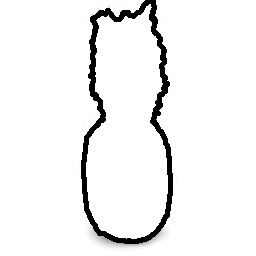
\includegraphics[width=.22\linewidth]{images/autocomplete_data_generation/original.png}} &
    \frame{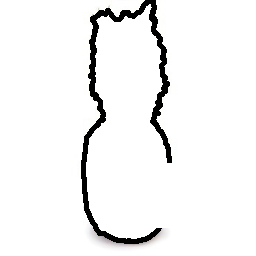
\includegraphics[width=.22\linewidth]{images/autocomplete_data_generation/64.png}} &
    \frame{
\includegraphics[width=.22\linewidth]{images/autocomplete_data_generation/128.png}} &
    \frame{
\includegraphics[width=.22\linewidth]{images/autocomplete_data_generation/192.png}}\\
    Outline &
    64x64&
    128x128 &
    192x192\\
\end{tabular} \\
    \caption{\textbf{Autocomplete Training Data Creation:} 3 sizes (64$\times$64,128$\times$128,192$\times$192) of white colored occluders were used for simulating partial edges.}
    \label{fig:autocomplete_data_generation}
\end{figure}

\begin{figure*}[t]
    \centering
    % 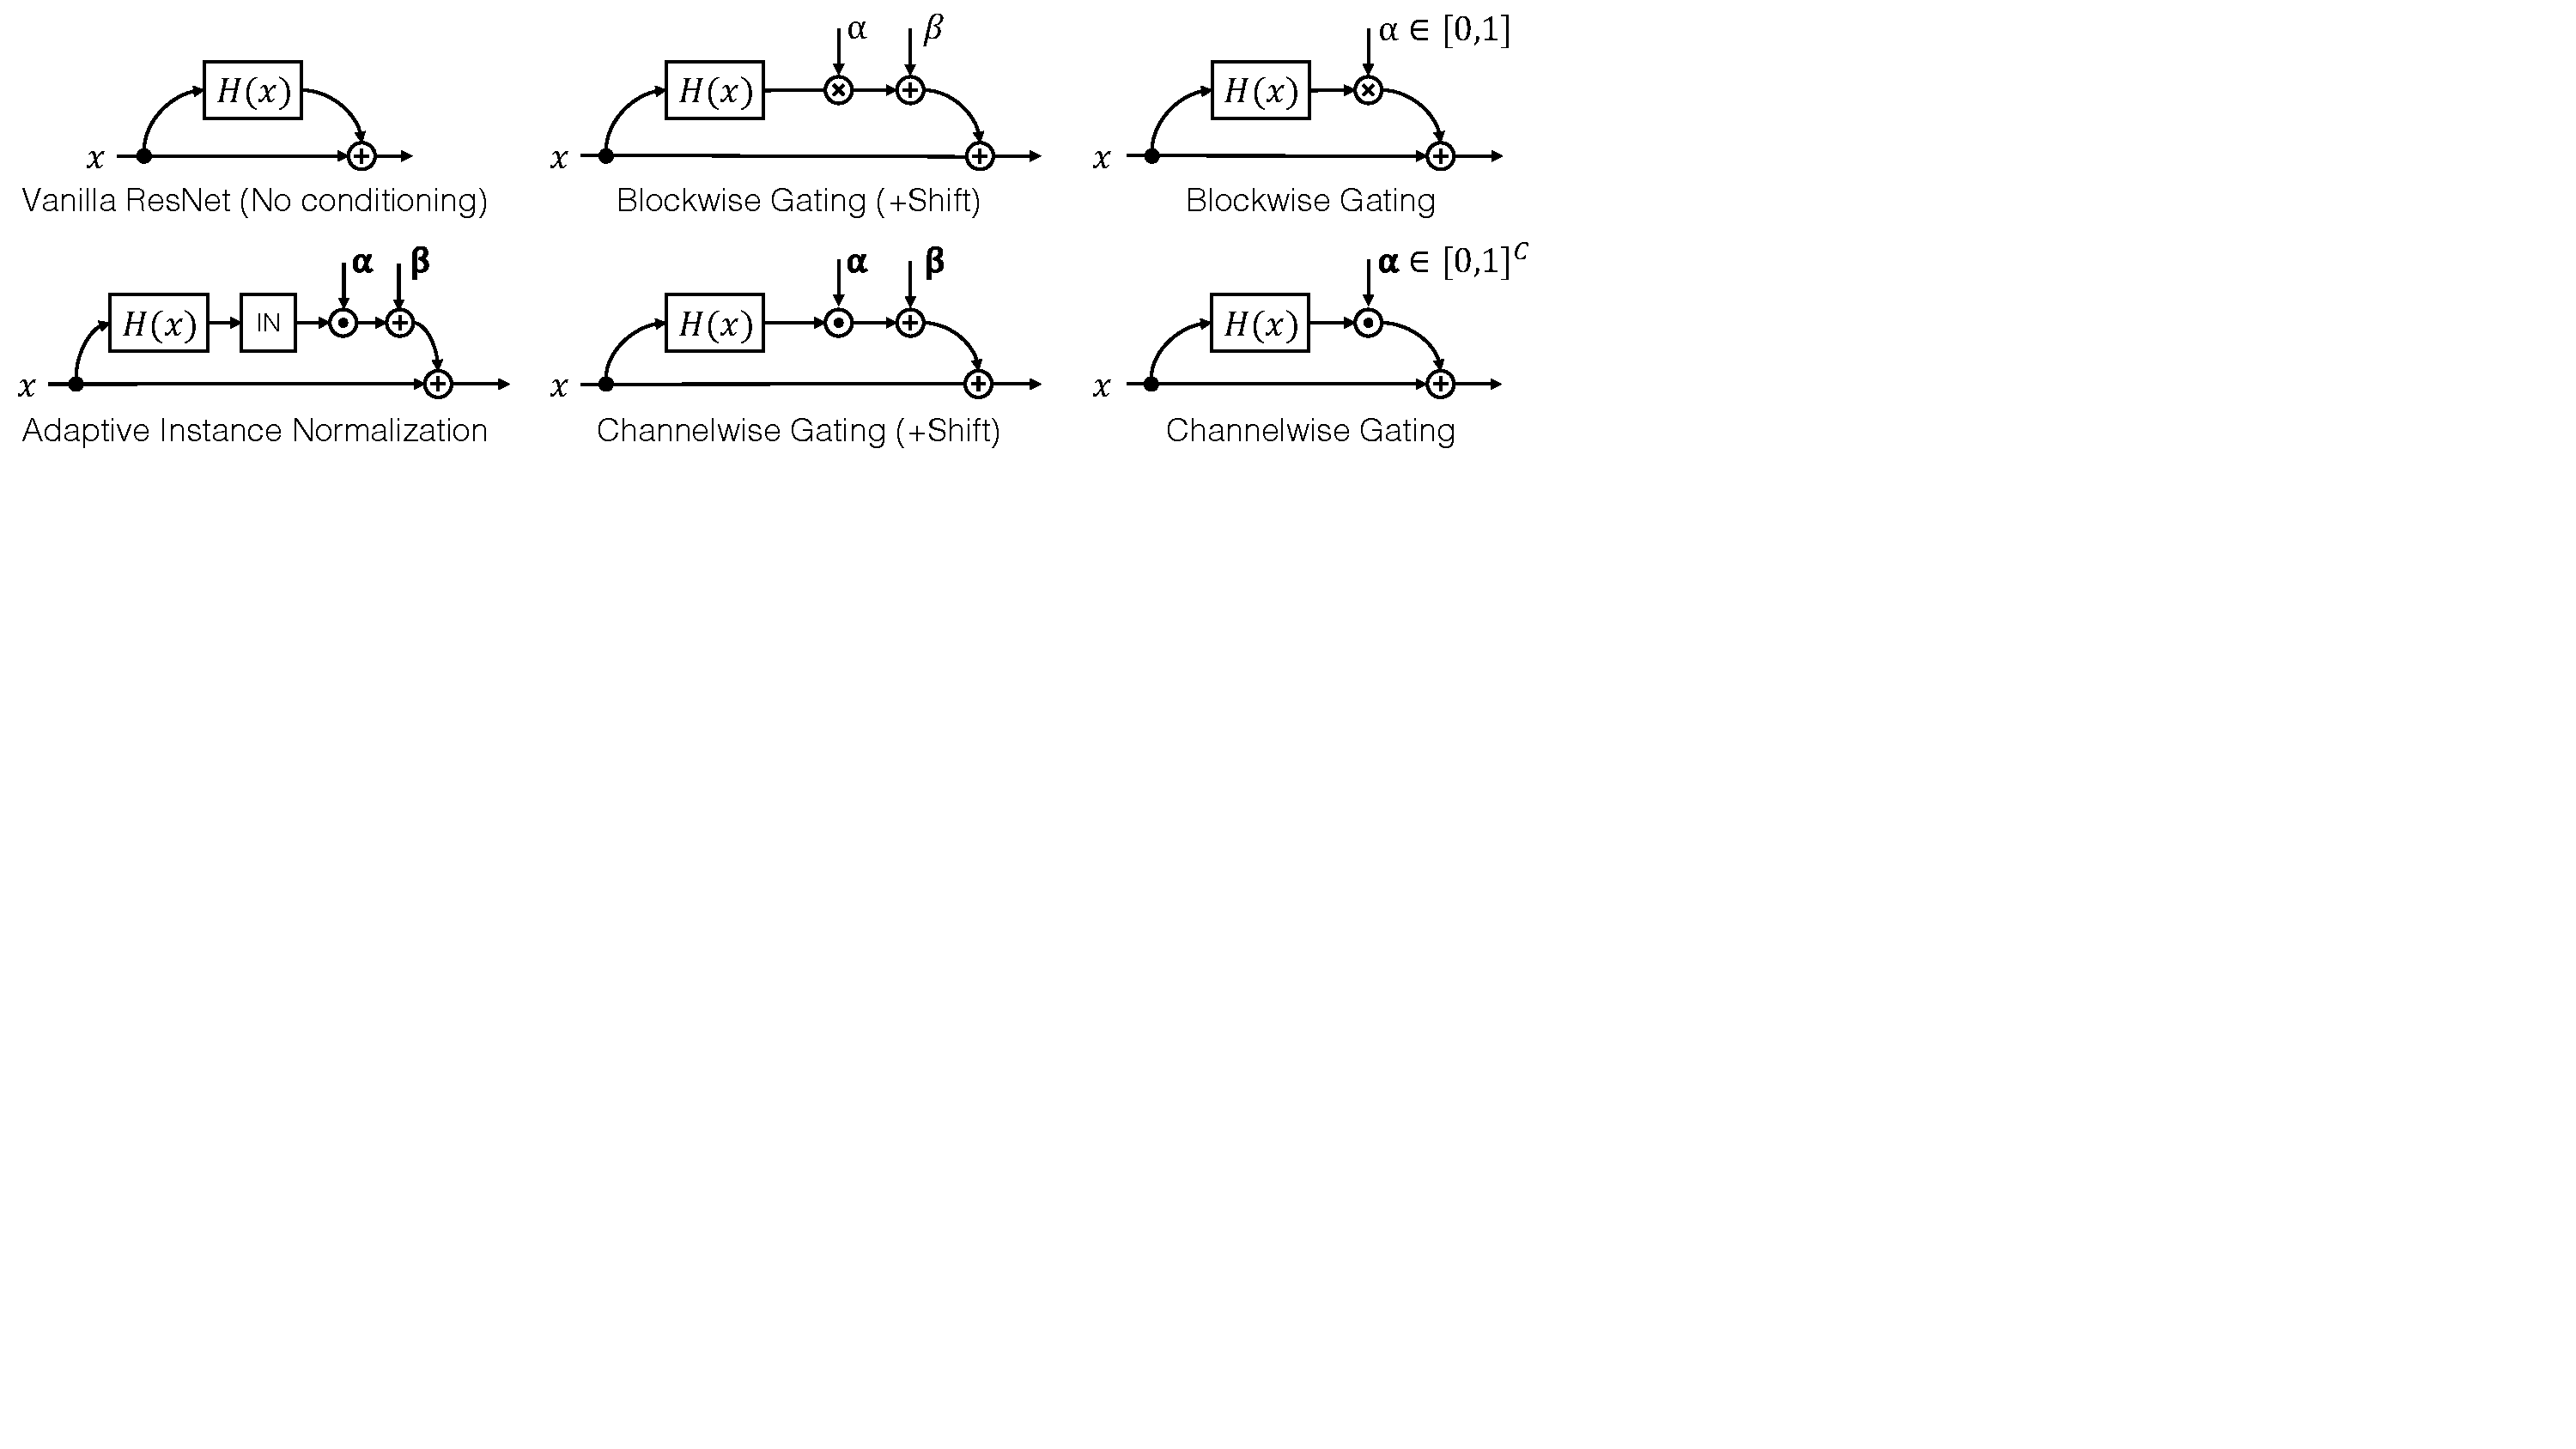
\includegraphics[width=\linewidth]{paper_images/arch_gate.pdf}
    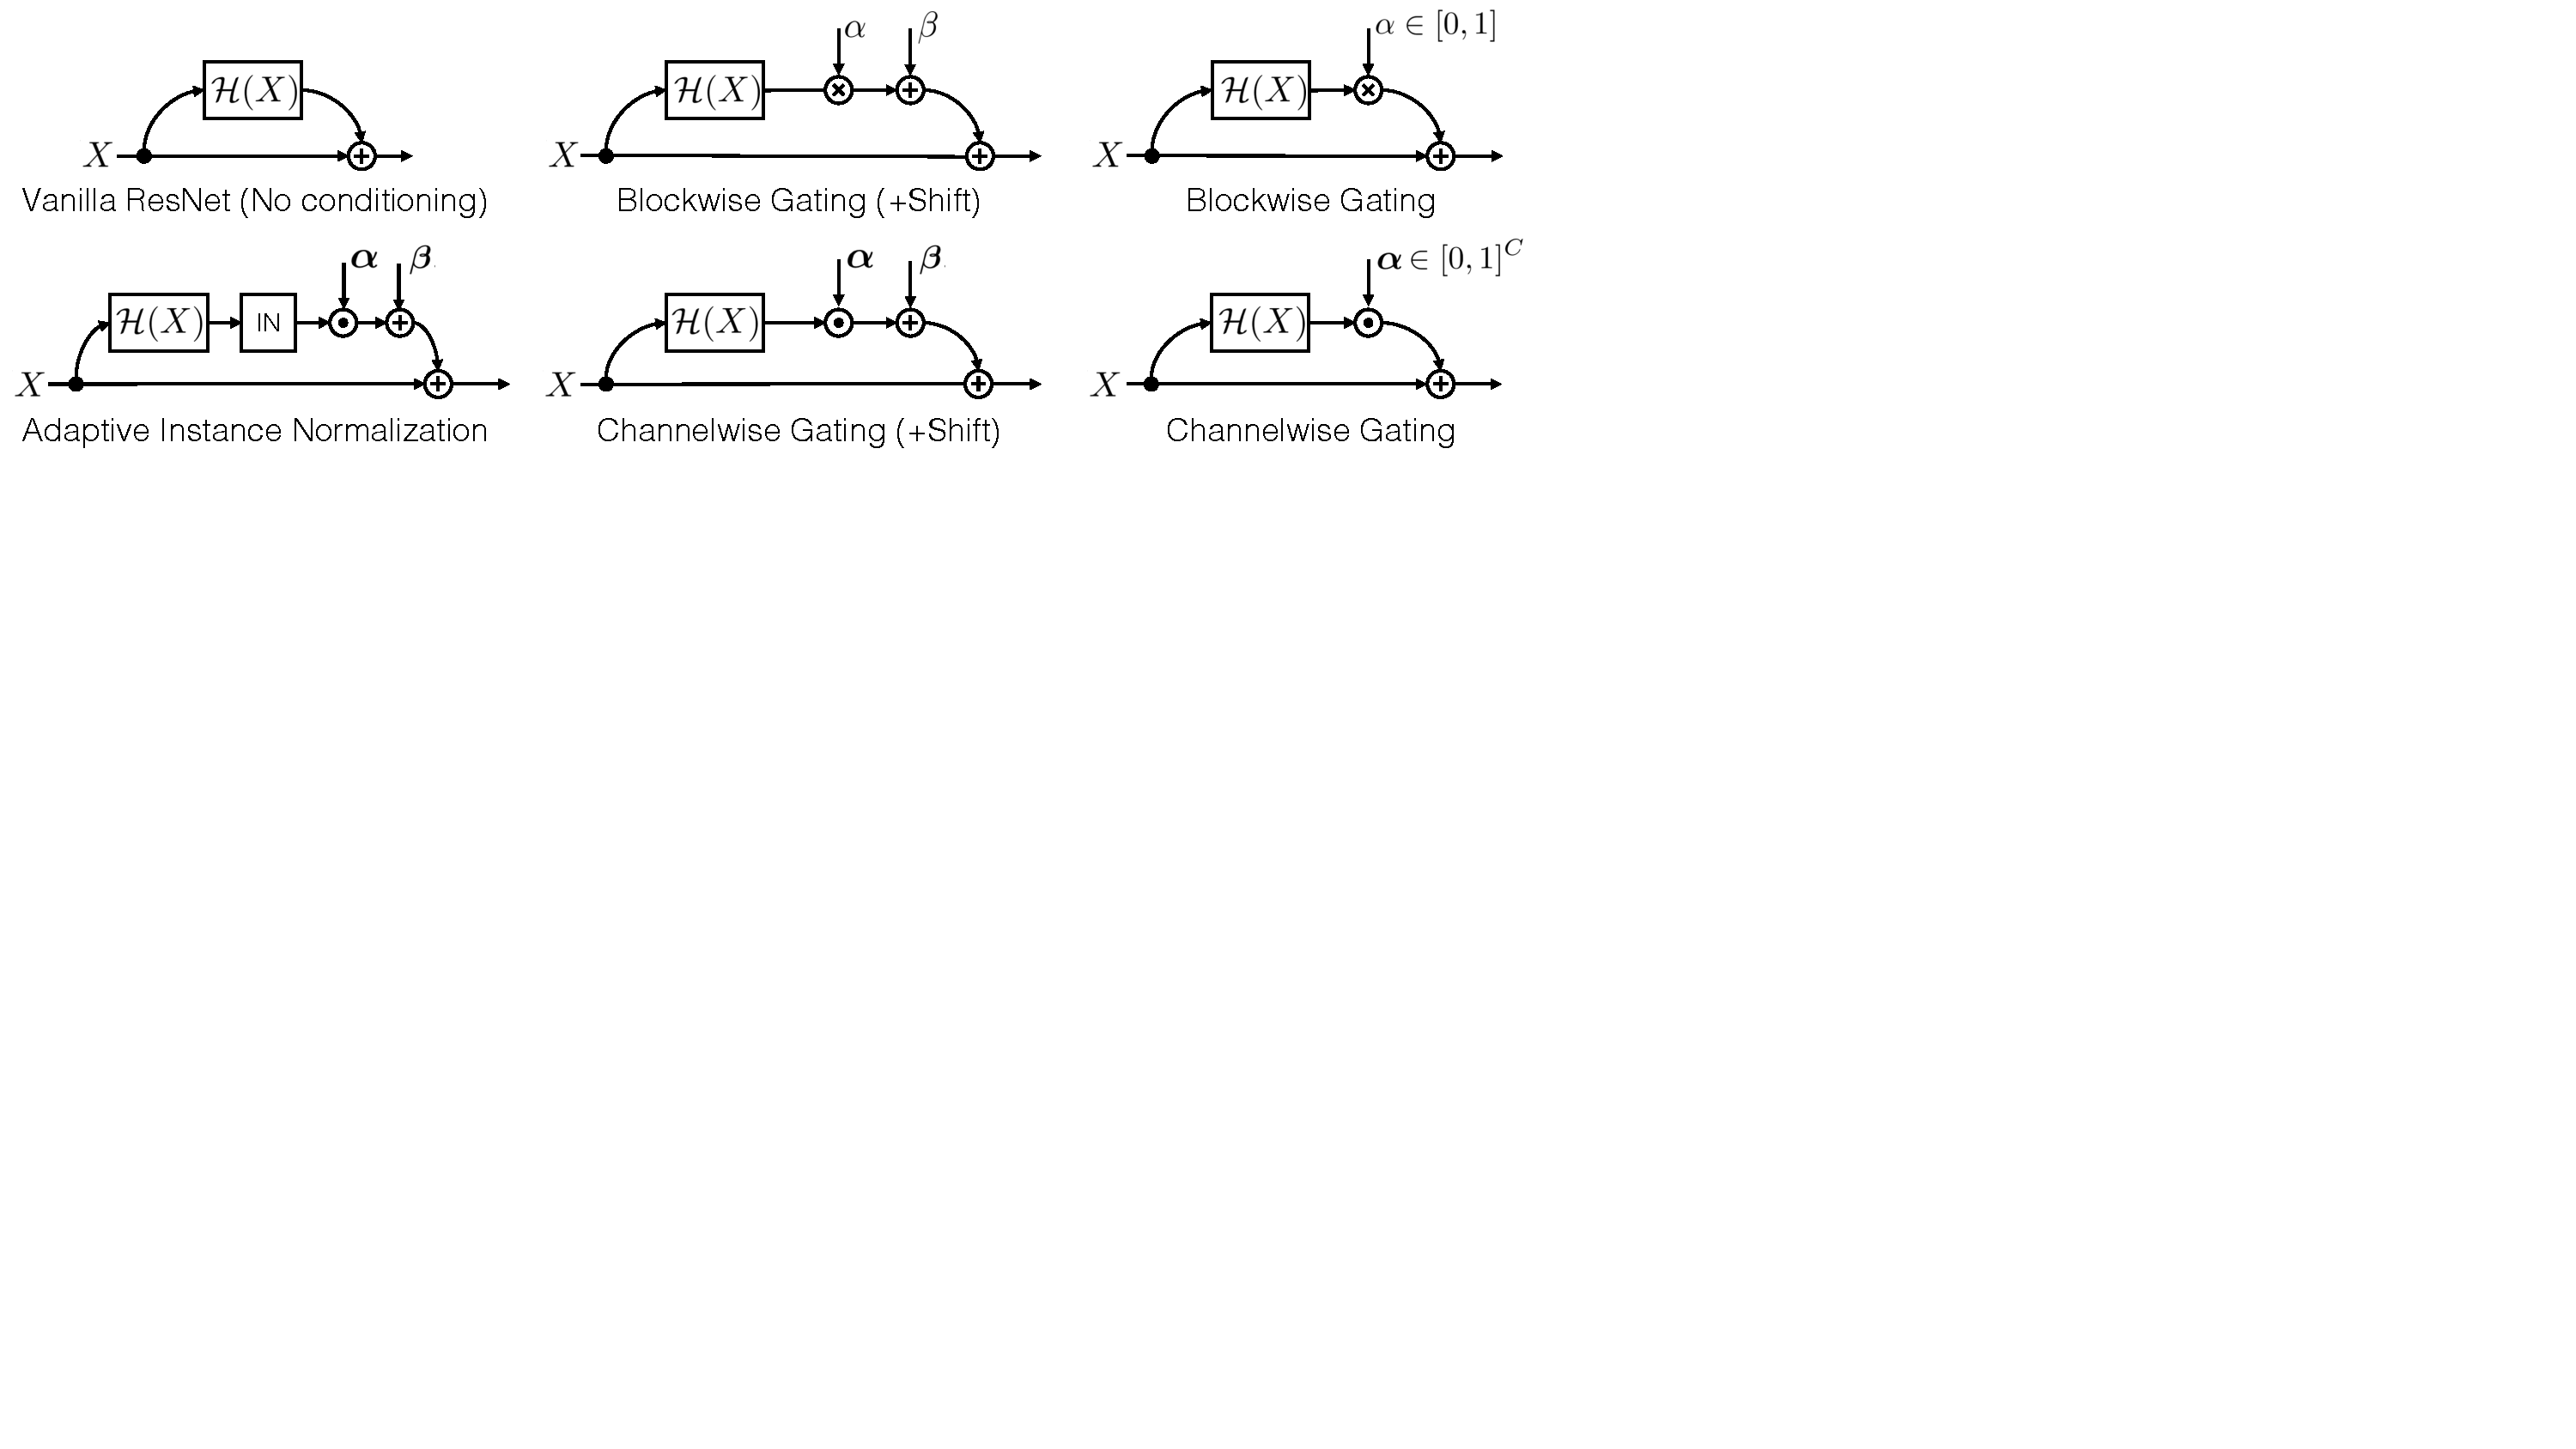
\includegraphics[width=1.\linewidth]{paper_images/arch_gate2.pdf}
    \caption{
    % {\bf Incorporating soft-gating into residual blocks.} \rz{Order got changed, may or may not need to add key for hadamard product}
    {\bf (Top-left)} A ``vanilla" residual block without gated conditioning parameters modifies input tensor $X$ into $X+\mathcal{H}(X)$. Conditioning with concatenation uses this setup. {\bf (Top-mid)} The $\mathcal{H}(X)$ block is softly-gated by scalar parameter $\alpha$ and shift $\beta$. {\bf (Top-right)} Only the gating is used, without bias. {\bf (Bot-left)} Adaptive Instance Normalization~\cite{huang2017arbitrary} applies a channel-wise scaling and shifting after an instance normalization layer. {\bf (Bot-mid)} Channel-wise gating adds restrictions to the range of $\mbox{\boldmath $\alpha$}$. {\bf (Bot-right)} We find that channel-wise gating (without added bias) to empirically produce the best results.\label{fig:arch-gate}
    \vspace{-2mm}
    }
    % \vspace{-4mm}
\end{figure*}


\begin{figure*}[t]
    \centering
    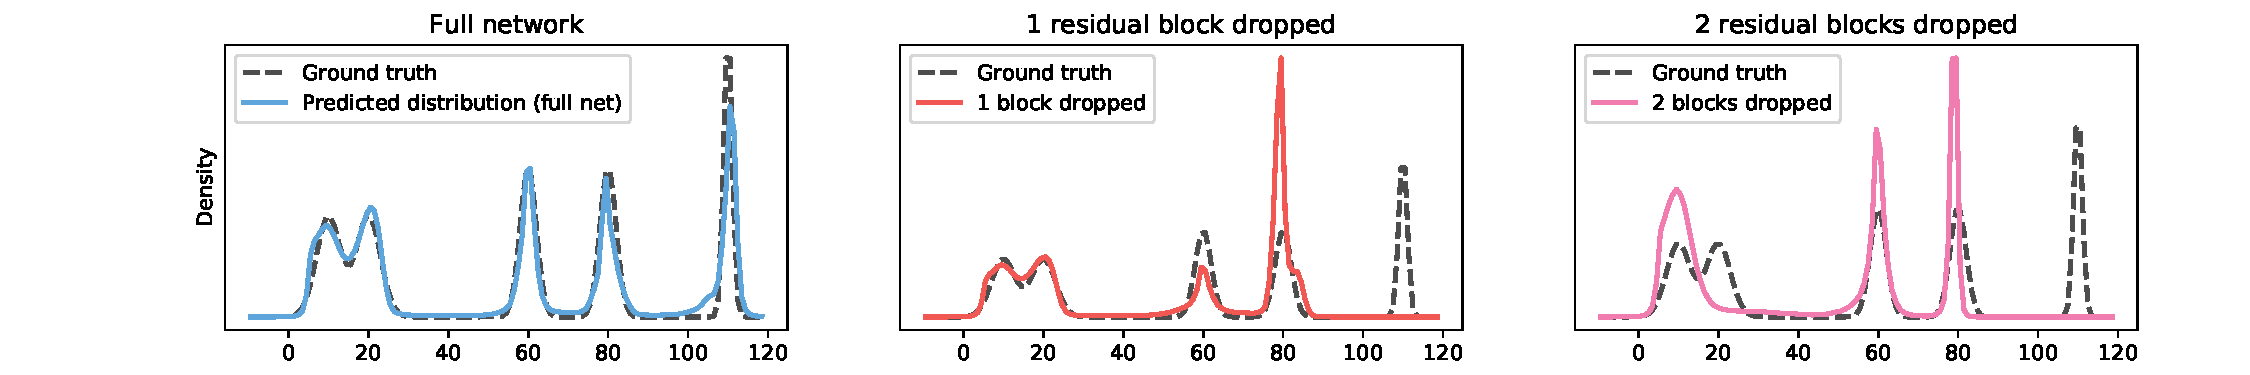
\includegraphics[width=\linewidth,trim={2.6cm 0 1.8cm 0},clip]{paper_images/mog.pdf}
    % 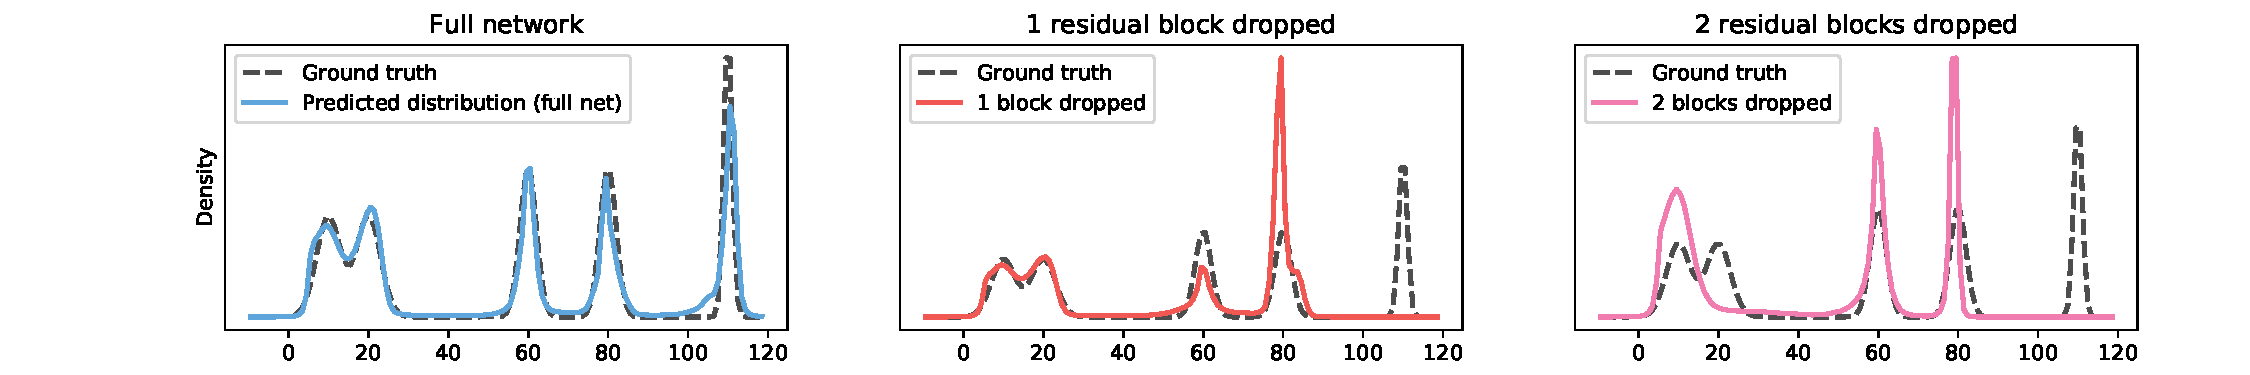
\includegraphics[width=\linewidth]{paper_images/mog.pdf}
    \caption{{\bf 1D Mixture of Gaussians.} {\bf (Left)} Samples from a residual network (blue-dotted) closely approximate the training distribution (black). {\bf (Mid)} Removing one residual block removes one mode of the predicted distribution. {\bf (Right)} Removing two blocks drops two modes. Note that samples stay mostly ``on-manifold" of the ground truth distribution.
    %\vspace{-2mm}
    }\label{fig:onedexperiment}
    %\vspace{-3mm}
\end{figure*}

\subsection{Appearance synthesis}
%We use a conditional GAN formulation for generating images from outlines as shown by the efficacy in \cite{isola2016image2image,zhu2017toward}. 
An ideal interactive sketch-to-image system  should be able to generate multiple different image classes with a single generator. 
Beside memory and time considerations (avoiding loading/using a separate model per class, reduce overall memory), a single network can share features related to outline recognition and texture generation that are common across classes, which helps training with limited examples per class. %\es{Didn't we already said that in the intro? If yes we should remove/significantly shorten}

As we later show, existing class conditioning-by-concatenation techniques fail to properly condition the network about the class information in current image translation networks~\cite{isola2016image2image,zhu2017toward}.
%
To address this, we propose an effective soft gating mechanism, shown in Figure~\ref{fig:arch-gate}.
Conceptually, our network consists of a small external gating network that is conditioned on the object class (encoded as a 1-hot vector).
The gating network outputs parameters that are used to modify the features of the main generator network.
We now describe this architecture in detail.
%condition the main generator 
%control the bias and/or amount of activation of different layers/channels in a fully ResNet generation network~\cite{he2016deep} with added ResNet-like upsampling and downsampling layers. 
% Similar to \cite{karras2018style} we used a soft gating mechanism to properly condition the generator about the class condition using a gating hypernetwork which generated a map of how to use the various residual blocks based on the class conditioning. As shown in \figref{fig:arch-inj} we have all the layers implemented as resnet blocks and the gating hypernetwork decides how much ($\alpha$) of each block $f(x)$ to use via a simple gate $\alpha$ for a block i.e. the output of each block is now $x + \alpha f(x)$  where $\alpha \in [0,1]$. We explored certain variations of the above technique by introducing gating in the discriminator as well as generalizing from block-wise gating to channel-wise gating. For a complete analysis of the various forms of gating please refer to the supplementary material.
%
%The methods above do not fundamentally modify the structure of the network. 
In ResNets~\cite{he2016deep}, an input feature tensor $X_l$ is modified by function
\begin{equation}
X_{l+1} = X_l+\mathcal{H}_l(X_l).
\end{equation}
Changes in resolution are obtained by upsampling before or downsampling after the residual block.
%We investigate multiple variants of the \textit{learned} gating network.
% , as illustrated in Fig.~\ref{fig:arch-gate}.
% For visual clarity, we omit the layer subscript $l$ in feature tensor $X_l$, residual subnetwork $\mathcal{H}_l$, and the gating parameters $\alpha_l, \beta_l$.
Our gating network augments this with a predicted scalar $\alpha$ for each layer of the network using a learned network $\mathcal{F}({\bf y})$, where  ${\bf y}$ is the conditioning vector:
\begin{equation}
X + \alpha \; \mathcal{H}(X), \text{where } \alpha \in [0,1]
\end{equation}

If the conditioning vector ${\bf y}$ has no use for a particular block, it can predict $\alpha$ close to zero, and effectively switch off the layer.
% , and use that layer instead for other classes.
During training, blocks within the main network can transform the image in various ways, and $\mathcal{F}$ can modulate such that the most useful blocks are selected. 
Unlike previous feature map conditioning methods such as AdaIn~\cite{ulyanovinstance}, we apply gating to \emph{both} the generator and discriminator. 
This enables the discriminator to select blocks which effectively judge whether generations are real or fake, conditioned on the class input.
% Via accurate gradients backpropagated to the generator it also enables the generator to generate class conditioned high resolution image samples.
Some blocks can be shared across regions in the conditioning vector, whereas other blocks can specialize for a given class.

A more powerful method is to apply this weighting channel-wise using a vector {\boldmath$\alpha$}: % This is denoted as follows:
\begin{align}
X + \mbox{\boldmath $\alpha$} \odot \mathcal{H}(X), \text{where } \mbox{\boldmath $\alpha$} \in [0,1]^c 
\end{align}
Where $\odot$ represents channel-wise multiplication. This allows specific channels to be switched ``on" or ``off", providing additional degrees of freedom.
%We make the corresponding changes in the discriminator as well. 
%Soft-gating has been explored by Veit et al.~\cite{veit2018adaptive} in a classification setting. 
We found that this channelwise approach for gating provides the strongest results. 

We additionally explored incorporating a bias term after the soft-gating, either block-wise using a scalar $\beta \in [-1,1]$ per layer, or channel-wise using a vector $\mbox{\boldmath $\beta$} \in [-1, 1]^c$ per layer but we found that they did not help much, and so we leave them out of our final model.
% \ow{but found that they did not help much, and so we leave them out of our final model?}




Finally, we describe our network architecture. 
We base our architecture on the proposed residual \textbf{Encoder-Decoder} model from MUNIT~\cite{huang2018multimodal}.
This architecture, is comprised of 3 \texttt{conv} layers, 8 residual blocks, and 3 \texttt{up-conv} layers. The residual blocks have 256 channels. 
First, we deepen the network, based on the principle that deeper networks have more valid disjoint, partially shared, paths~\cite{veit2016residual}, and add 24 residual blocks. 
To enable the larger number of residual blocks, we drastically reduce the width to 32 channels for every layer. 
We refer to this network as \textbf{SkinnyResNet}. 
Additionally, we found that modifying the downsampling and upsampling blocks to be residual connections as well improved results, and also enables us to apply gating to {\em all} blocks. 
When gating is used, the gate prediction network, $\mathcal{F} ({\bf y})$,  
%Fig.~\ref{fig:arch-inj} (mid-right, right) 
is also designed using residual blocks. Additional architecture details are in the supplementary material. 

\begin{figure}[t]%[ht!]
\centering
\resizebox{1.0\linewidth}{!}{
\begin{tabular}{*{5}{c@{\hspace{3px}}}}
    \frame{
\includegraphics[width=.2\linewidth]{images/autocomplete_generate/scribble/basketball.png}} &
    %\frame{
\includegraphics[width=.10\linewidth]{images/autocomplete_generate/scribble/soccer.png}} &
    \frame{
\includegraphics[width=.2\linewidth]{images/autocomplete_generate/scribble/watermelon.png}} & 
    \frame{
\includegraphics[width=.2\linewidth]{images/autocomplete_generate/scribble/orange.png}}&
    \frame{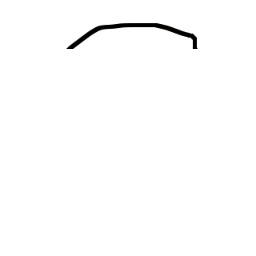
\includegraphics[width=.2\linewidth]{images/autocomplete_generate/scribble/cookie.png}} &
    %\frame{
\includegraphics[width=.10\linewidth]{images/autocomplete_generate/scribble/moon.png}} &
    %\frame{
\includegraphics[width=.10\linewidth]{images/autocomplete_generate/scribble/strawberry.png}} &
    \frame{
\includegraphics[width=.2\linewidth]{images/autocomplete_generate/scribble/pineapple.png}}
    %\frame{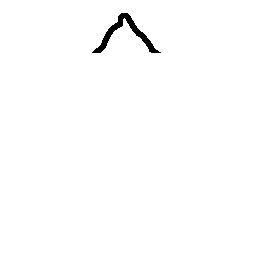
\includegraphics[width=.10\linewidth]{images/autocomplete_generate/scribble/cupcake.png}} &
    %\frame{
\includegraphics[width=.10\linewidth]{images/autocomplete_generate/scribble/chicken.png}}
    \\
    
    \frame{
\includegraphics[width=.2\linewidth]{images/autocomplete_generate/autocomplete/basketball.png}} &
    %\frame{
\includegraphics[width=.10\linewidth]{images/autocomplete_generate/autocomplete/soccer.png}} &
    \frame{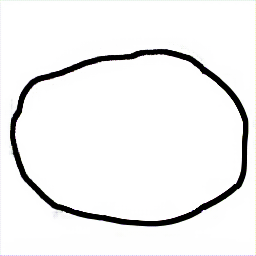
\includegraphics[width=.2\linewidth]{images/autocomplete_generate/autocomplete/watermelon.png}} & 
    \frame{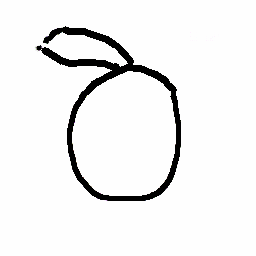
\includegraphics[width=.2\linewidth]{images/autocomplete_generate/autocomplete/orange.png}}&
    \frame{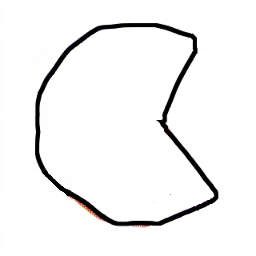
\includegraphics[width=.2\linewidth]{images/autocomplete_generate/autocomplete/cookie.png}} &
    %\frame{
\includegraphics[width=.10\linewidth]{images/autocomplete_generate/autocomplete/moon.png}} &
    %\frame{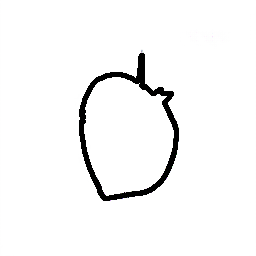
\includegraphics[width=.10\linewidth]{images/autocomplete_generate/autocomplete/strawberry.png}} &
    \frame{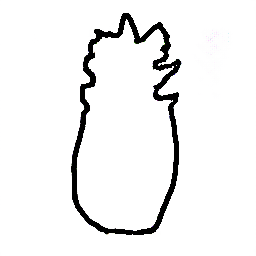
\includegraphics[width=.2\linewidth]{images/autocomplete_generate/autocomplete/pineapple.png}}
    %\frame{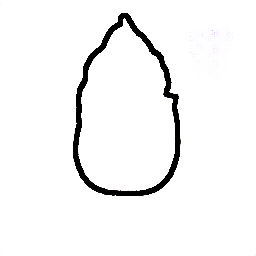
\includegraphics[width=.10\linewidth]{images/autocomplete_generate/autocomplete/cupcake.png}} &
    %\frame{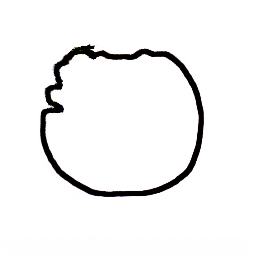
\includegraphics[width=.10\linewidth]{images/autocomplete_generate/autocomplete/chicken.png}}
    \\
    
    
    \frame{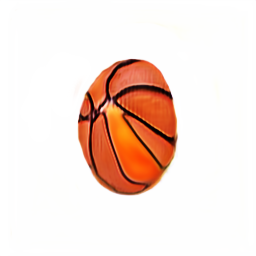
\includegraphics[width=.2\linewidth]{images/autocomplete_generate/image/basketball.png}} &
    %\frame{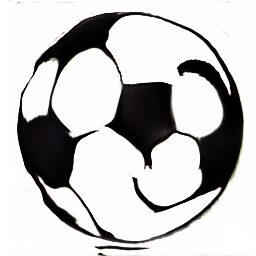
\includegraphics[width=.10\linewidth]{images/autocomplete_generate/image/soccer.png}} &
    \frame{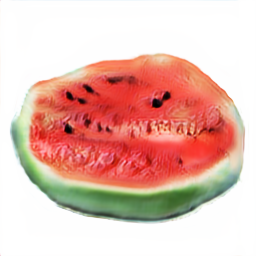
\includegraphics[width=.2\linewidth]{images/autocomplete_generate/image/watermelon.png}} & 
    \frame{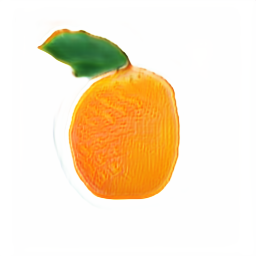
\includegraphics[width=.2\linewidth]{images/autocomplete_generate/image/orange.png}}&
    \frame{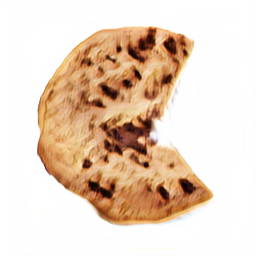
\includegraphics[width=.2\linewidth]{images/autocomplete_generate/image/cookie.png}} &
    %\frame{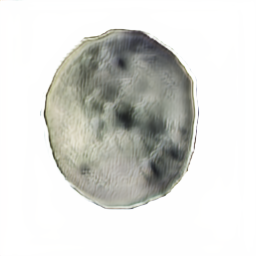
\includegraphics[width=.10\linewidth]{images/autocomplete_generate/image/moon.png}} &
    %\frame{\includegraphics[width=.10\linewidth]{images/autocomplete_generate/image/strawberry.png}} &
    \frame{\includegraphics[width=.2\linewidth]{images/autocomplete_generate/image/pineapple.png}}
    %\frame{\includegraphics[width=.10\linewidth]{images/autocomplete_generate/image/cupcake.png}} &
    %\frame{\includegraphics[width=.10\linewidth]{images/autocomplete_generate/image/chicken.png}}
    \\
    % \begin{subfigure}[t]{.15\linewidth}\caption{}\label{fig:basketball_partial}\end{subfigure} &
    % \begin{subfigure}[t]{.15\linewidth}\caption{}\label{fig:basketball_full}\end{subfigure} &
    % \begin{subfigure}[t]{.15\linewidth}\caption{}\label{fig:soccer_partial}\end{subfigure} &
    % \begin{subfigure}[t]{.15\linewidth}\caption{}\label{fig:soccer_full}\end{subfigure} &
    % \begin{subfigure}[t]{.15\linewidth}\caption{}\label{fig:cupcake_partial}\end{subfigure} &
    % \begin{subfigure}[t]{.15\linewidth}\caption{}\label{fig:cupcake_full}\end{subfigure}\\
\end{tabular}
}
    \caption{\textbf{Sketch \& Fill results}.
    A few input strokes in the first row are enough to automatically complete the class specific outlines and appearance. }
    % \es{replace orange and chicken. maybe also moon and cupcake.}}
    \label{fig:autocomplete_generate}
    %\vspace{-3mm}
\end{figure}


\begin{figure}[t]%[ht!]
\centering
\small
\begin{tabular}{*{3}{c@{\hspace{3px}}}}
    \frame{ \includegraphics[width=.30\linewidth]{images/ablation_shoes/partial_outline.png}} &
    \frame{\includegraphics[width=.30\linewidth]{images/ablation_shoes/trained_partial_edges.png}} &
    \frame{\includegraphics[width=.30\linewidth]{images/ablation_shoes/trained_partial_outlines.png}}
    \\
    Input & PE trained & PO trained \\
    % %
    % \begin{subfigure}[t]{.30\linewidth}\caption{Input}
    % \label{fig:basketball_partial}\end{subfigure} &
    % \begin{subfigure}[t]{.30\linewidth}\caption{PE trained} \label{fig:basketball_full}\end{subfigure} &
    % \begin{subfigure}[t]{.30\linewidth}\caption{PO trained} \label{fig:soccer_partial}\end{subfigure} \\
    % %
    \frame{\includegraphics[width=.30\linewidth]{images/ablation_shoes/autocompleted.png}} &
    \frame{\includegraphics[width=.30\linewidth]{images/ablation_shoes/pretrained_test_autocompleted.png}} &
    \frame{\includegraphics[width=.30\linewidth]{images/ablation_shoes/test_autocompleted.png}} 
    \\
    Input & FE trained & FO trained \\
    % \begin{subfigure}[t]{.30\linewidth}\caption{\textbf{Completion}} \label{fig:soccer_full}\end{subfigure} &
    % \begin{subfigure}[t]{.30\linewidth}\caption{FE trained}\label{fig:cupcake_partial}\end{subfigure} &
    % \begin{subfigure}[t]{.30\linewidth}\caption{\textbf{FO trained}} \label{fig:cupcake_full}\end{subfigure}\\
\end{tabular} \\
\normalsize
\vspace{-2mm}
    \caption{\textbf{Efficacy of outlines:} Networks trained on partial edges (PE) produce worse quality results than those trained on partial outlines (PO) when applied to real human input (top). Similarly, an appearance synthesis model trained on full edges (FE) does not work as well as a network trained on full outlines (FO) when given simplified sketches as input (bottom).}
    \label{fig:ablation_partialedge_full_outline}
\end{figure}


\subsection{Insights on Gating Mechanism}
We demonstrate the intuition behind this type of gating by a toy experiment in ~\figref{fig:onedexperiment} where a generative network models a one dimensional mixture of Gaussians, comprised of five components. 
For this test, the generator and discriminator architectures consist of only residual blocks, where each residual block is composed of fully connected layers. 
Additional details are in the supplementary material. 

The generator is conditioned on a latent vector $z$, and is trained to approximate the distribution, as seen in Fig.~\ref{fig:onedexperiment} (left). 
Removing a single residual block, in the spirit of~\cite{veit2016residual}, leads to the disappearance of a mode from the predicted distribution. 
Removal of another block leads to further removal of another mode, as seen in Fig.~\ref{fig:onedexperiment}  (mid, right). 
The purpose of the gating network, thus, is to enable the network to learn which blocks (or more specifically, which channels) to attend to for each object class. %It increases the participation of the condition $({\bf y})$ in the generation process which in turn helps the network to effectively disentangle different object classes.
%This experiment shows an encouraging result, suggesting that residual blocks decompose naturally into modeling parts of a distribution.





% \section{Method}
% Interactive Image Generation can be thought of as a sequence of constraints given by the user and the subsequent addition of more constraints based on the geometry or texture constraints provided by the user. In such a constraint based setting a Generative Model has the freedom to choose how to generate a realistic real image honoring the constraints and allowing the freedom to generate as realistically as possible in the unconstrained areas. A system which can generate realistic final images starting from few strokes acting as constraints and honoring constraints at all times would be interactive provided we have fast enough feedforward processing through the network.

% \paragraph{Preliminaries:}
% We can formalize the process of user interaction at the different instances of the interaction, each stroke image at the $i^{th}$ step of the user interaction is $S_i$ representing the user constraints expressed at the $i^{th}$ step of the generation process. $S_i$ can be expressed as a subset of strokes from the set of edges $E$ or from the set of outlines $O$ . $C_i$ is the automatically completed constraint image, completed from the Stroke Image $S_i$ . $G_i$ is the generated image generated by the network after the $i^{th}$ constraint addition step.

% \paragraph{Naive Approaches:}
% As introduced in pix2pix \cite{isola2016image2image} $S_i$ could be from the set of edge maps $E$ but as shown in the experiments section the automatic completion of the constraint image $C_i$ and the subsequent generated image $G_i$ becomes hard in this setting. For instance in case of a partial sketch it'd be hard to discern whether a partial edge is part of the outline of the object or just a texture stroke inside the image hence hindering in the task of interactive image generation. Another naive approach could be to represent the constraint image $S_i$ as a partial outline and generate the full image from the partial outline. There's a reduction in the quality of generations achieved apart from the fact that the automatically completed constraint image $C_i$ further guides the user for better edits to the final image thus granting more control on the generation process.

% \paragraph{Approach:}
% We adopt a two step approach, and restricting the constraint sketches $S_i$ to be from the set of outlines $O$. The first step constitutes of the automatic completion of the constraint sketch $C_i$ from $S_i$ which has to honor the constraints the user has already made in $S_i$ and make sure that the completed constraint sketch $C_i$ is a valid constraint sketch from the domain of valid constraint outlines $O$. We start experiments on the existing datasets of handbags \cite{zhu2016generative} and shoes \cite{yu2014fine}. In these settings the outline would be enough to discern whether the user would like to generate a handbag or a shoe but moving forward in the direction of interactive image generation the user would like to have the option of generating multiple classes and not just a single class. Moving onto multiple classes poses the additional challenge that multiple classes might have similar outlines for instance circular objects such as soccerballs, basketballs and moons have similar outlines which are quite circular. In such a scenario the input constraint sketch $S_i$ or the automatically completed outline $C_i$ is not enough to guide the generation towards the correct class $y$ for the generation. Traditional Image to Image settings fail in proper injection of high dimension information in terms of the source image $S_i$ or $C_i$ with low dimensional class-conditioning information $y$. To properly condition the network in this setting with the class $y$ we introduce a gating hypernetwork \cite{karras2018style} which would be described in the next section.

% \section{Gated Generative Adversarial Network}
% \label{sec:methods}
% We consider image-to-image translation problems, mapping input image $A$ to output $B \in \mathds{R}^{h\times w\times 3}$, with the benefit of a conditioning vector ${\bf y} \in \mathds{R}^{d}$. We learn this mapping with multilayer generator $\mathcal{G}(A,{\bf y})$ to produce output $\widehat{B}$. We refer to the feature map at each channel as $X_l\in \mathds{R}^{h_l\times w_l\times c_l}$, where $h_l \times w_l$ is the spatial size of the feature map, and $c_l$ is the number of channels in the layer. 
% % The total channels in the network is $C = \sum_l C_l$. 
% The conditioning vector ${\bf y}$ can be categorical, expressed as a 1-hot vector, or a continuous vector. 
% % , ground truth output $B \in \mathds{R}^{H\times W\times 3}$, generator $\mathcal{G}$, output $\widehat{B}=\mathcal{G}(A,y)$.
% % \subsection{Conditioning injection variants}
% The way that ${\bf y}$ is integrated into the network plays a critical role. We systematically explore several variants, as illustrated in Fig.~\ref{fig:arch-inj}.

% % There are many ways that the conditioning vector $\bf y$ can be integrated into the network. 

% \subsection{Naive concatenation}
% The most straightforward method is to spatially replicate the vector into a tensor of appropriate size and concatenate it to the input layer~\cite{zhu2017toward,choi2017stargan}. A potential weakness
% % of concatenating at the {\em input only}
% is the large distance between the conditioner and the output, which can lead to the generator easily ignoring the conditioner during learning. A previously explored solution~\cite{zhu2017toward} is to simply concatenate the conditioner into every layer.

% \subsection{Recovering the conditioning vector}

% % \paragraph{Auxiliary classifier or latent regressor for conditioning vector recovery}
% A technique for encouraging adherence to the conditioner is through the objective function. As seen in Fig.~\ref{fig:arch-inj}, a hypernetwork $\mathcal{Q}$ predicts conditioner from output image $\widehat{B}$. 
% % A loss is added to the optimization between ground truth $y$ and predicted $\hat{y}$, and has been explored in 
% The added loss between ground truth ${\bf y}$ and predicted $\hat{ {\bf y}}$ encourages the output to contain information about the conditioner. This has been previously explored in both the class-conditional~\cite{odena2016conditional,choi2017stargan,salimans2016improved} and latent code-conditional settings~\cite{chen2016infogan,donahue2016adversarial,zhu2017toward}. In our experiments, we find that this technique improves upon naive concatenation. We further explore a complementary approach, modifying the architecture of the main generator.

% % \ow{what is the problem with the above approach that leads us to propose the next}
% % \eli{I added a sentence but maybe we can say something stronger? Did we ever try ACGAN on the multi-class task? If yes and it didn't work, maybe mention here?}

% \subsection{Conditioning with Soft-Gating (Proposed)}
% \paragraph{Conditioning with Soft-Gating (Proposed)}
% %The methods above do not fundamentally modify the structure of the network. 
% In ResNets, an input feature tensor $X_l$ is modified by function $X_{l+1} = X_l+\mathcal{H}_l(X_l)$.
% Changes in resolution are obtained by upsampling before or downsampling after the residual block.
% We investigate multiple variants of the \textit{learned} gating network, as illustrated in Fig.~\ref{fig:arch-gate}.
% For visual clarity, we omit the layer subscript $l$ in feature tensor $X_l$, residual subnetwork $\mathcal{H}_l$, and the gating parameters $\alpha_l, \beta_l$.

% We begin by predicting a scalar $\alpha$ using a learned network $\mathcal{F}({\bf y})$ for each layer of the network:

% % We now begin to describe our model which we call Gated Generative Adversarial Networks (GAN-Gate). It is primarily based on an interesting experiment whereby \cite{veit2016residual} showed that the residual networks behave as an ensemble of several shallower networks, and removing a few residual blocks at test time performed highly competitive to the original network itself. This implies that, perhaps, given a GAN architecture with residual blocks as its components, it is possible to {\em automatically} learn a mixture of shallower networks {\em conditioned} on the modes of the data distribution or the tasks we are interested in. This is exactly the objective that GAN-Gate achieves. More precisely, it automatically learns a mixture of shallower networks where each mixture component (a shallow network) is focused on generating data either from a mode or a task; depending on whether we are interested in {\em intraclass} or {\em interclass} variations. To this end, we first propose an architecture for GANs entirely based on residual blocks which is capable of generating highly competitive samples form image-to-image translation task compared to other baselines. Then, we propose to use a simple yet powerful {\em gating mechanism} over a subset of residual blocks where the gating automatically decides which blocks to {\em focus on} for a given condition. Note, this gating is learned automatically from the data. In the end, we also show that the gating mechanism provides an effective way to maximize mutual information in the {\em InfoGAN} objective, which otherwise was not possible.

% \vspace{-2mm}
% \begin{equation}
% X + \alpha \; \mathcal{H}(X), \text{where } \alpha \in [0,1]
% \end{equation}

% If the conditioning vector ${\bf y}$ has no use for a particular block, it can predict $\alpha$ close to zero, and effectively switch off the layer.
% % , and use that layer instead for other classes.
% During training, blocks within the main network can transform the image in various ways, and $\mathcal{F}$ can modulate such that the ``right" blocks are selected. We can also apply the operation channel-wise, using a vector {\boldmath$\alpha$}: % This is denoted as follows:

% \vspace{-4mm}
% \begin{align}
% X + \mbox{\boldmath $\alpha$} \odot \mathcal{H}(X), \text{where } \mbox{\boldmath $\alpha$} \in [0,1]^c 
% \end{align}

% Symbol $\odot$ respresents channel-wise multiplication. This provides additional degrees of freedom, allowing specific channels to be switched ``on" or ``off". We make the corresponding changes in the discriminator as well. 
% %Soft-gating has been explored by Veit et al.~\cite{veit2018adaptive} in a classification setting. 
% Intuitively, in GANs, this can enable the discriminator to select blocks which effectively judge whether generations are real or fake, conditioned on the class input.
% % Via accurate gradients backpropagated to the generator it also enables the generator to generate class conditioned high resolution image samples.
% Some blocks can be shared across regions in the conditioning vector, whereas other blocks can specialize for a given class.

% We empirically find that channel-wise gating provides the strongest results. 
% For completeness, we additionally explore incorporating shifting after the soft-gating, either block-wise using a scalar $\beta \in [-1,1]$ per layer, or channel-wise using a vector $\mbox{\boldmath $\beta$} \in [-1, 1]^c$ per layer.

%\rz{sentence summarizing why or how}
% \begin{equation}
% \text{AdaIn}(x, \alpha, \beta) = \alpha \big(\frac{x-\mu(x)}{\sigma(x)}\big)+\beta
% \label{eqn:adain}
% \end{equation}

% AdaIn layers perform a similar gating task. An Instance Normalization~\cite{ulyanovinstance} (IN) is applied before scaling and shifting the feature distribution. We constrain each element of {\boldmath $\alpha$} and {\boldmath $\beta$} in $[-1, 1]$\footnote{constraining between \( [0, 1] \) did not provide the best empirical results.}.

% \vspace{-2mm}
% \begin{equation}
% X + \mbox{\boldmath $\alpha$} \odot \text{IN} (\mathcal{H}(X)) + \mbox{\boldmath $\beta$}
% \end{equation}

% % \begin{figure*}[t]
% %     \centering
% %     \addSubFigThird{Picture2}{Ground Truth Distribution }{fig:1d_ground} 
% %     \addSubFigThird{Picture33.png}{Generated Samples from the trained Generator}{fig:1d_gen} 
% %     \addSubFigThird{Picture3.png}{Generated Samples from the trained Generator with one of the blocks removed}{fig:1d_gen_rem} 
% %     \caption{{\bf 1D Mixture of Gaussians experiment}}
% %     \label{fig:onedexperiment}
% %     \vspace{-3mm}
% % \end{figure*}


% \begin{figure*}[t]
%   \centering
%   \begin{minipage}[t]{0.48\linewidth}  
%   \centering
%   \resizebox{0.9\linewidth}{!} {
%   \setlength{\tabcolsep}{6pt}
%   \begin{tabular}{l c c c c}
%   \toprule
%     \multirow{3}{*}{\textbf{Method}} & \multicolumn{2}{c}{ {\bf SkinnyResNet}} & \multicolumn{2}{c}{ {\bf EncDec}} \\ \cmidrule(l){2-3} \cmidrule(l){4-5}
% % 	& \textbf{Accuracy} & \textbf{Realism} & \textbf{Accuracy} & \textbf{Realism} \\
% 	& Class. & AMT Fool. & Class. & AMT Fool. \\
% 	& Acc [\%] & Rate [\%] & Acc [\%] & Rate [\%] \\ \midrule
% % 	\cmidrule(l){1-1} \cmidrule(l){2-3} \cmidrule(l){4-5}
%     Ground truth & 100.0 & 50.0 & 100.0 & 50.0 \\ \midrule
%     1 gen/class & \textbf{\textit{97.0}} & 17.7$\pm$1.46 & -- & -- \\ \midrule
%     Concat (In)	& 62.6 & 15.0$\pm$1.4 & 39.2 & 7.5$\pm$1.06 \\ 
%     Concat (All) & 64.5 & 15.3$\pm$1.41 & 51.4 & 5.4$\pm$0.88 \\ \midrule
%     Cat(In)+Aux-Class & 65.6 & 14.5$\pm$1.5 & -- & -- \\ 
%     Cat(All)+Aux-Class & 67.0 & 19.7$\pm$1.42 & -- & --\\ \midrule
%     BlockGate(+bias) & 89.6 & 19.6$\pm$1.34 & -- & --\\ 
%     BlockGate & {\bf 99.6} & 17.3$\pm$1.61 & -- & --\\ 
%     AdaIn & 94.5 & 14.9$\pm$1.47 & -- & --\\ 
%     ChanGate(+bias) & 94.1 & 14.8$\pm$1.43 & -- & --\\ 
%     ChanGate & \textbf{\textit{97.0}} & {\bf 23.4$\pm$1.99} & 92.7 & 14.1$\pm$1.48 \\ 
% 	\hline
% 	\end{tabular} } 
%   \end{minipage}\begin{minipage}[]{0.48\linewidth}
%   \centering
%   \includegraphics[width=.9\linewidth]{paper_images/gen_real_vs_acc.pdf} 
%   \end{minipage}
%   \caption{\small {\bf Accuracy vs Realism on Outline$\rightarrow$Image task.} We measure generation accuracy by using a pretrained network to check whether the generated image is of the correct class and realism using the user-judged real vs. fake test from ~\cite{zhang2016colorful,isola2016image2image} conducted on Amazon Mechanical Turk (AMT). Higher is better for both metrics. Our SkinnyResNet architecture outperforms the Encoder-Decoder network, inspired by MUNIT~\cite{huang2018multimodal}. We perform a thorough ablation on our architecture, and find that channel-wise gating achieves high accuracy and higher realism. The right figure shows the correlation between the two tasks.
%   \vspace{-4mm}
%   }
%   \vspace{-3mm}
%   \label{fig:acc_vs_real}
% \end{figure*}


% % \subsection{Information Theoretic Benefits of Gating}
% \subsection{Effective Conditioning Injection as Mutual Information Preservation}
% \label{sec:infoGAN} 
% Injecting ${\bf y}$ at various layers essentially glues the generation with the conditioning.
% This helps in avoiding the pathological situation whereby disentanglement over the classes or modes suffer due to an easier approximation, $G(A,y) \approx G(A), \forall y$, learned by the generator. This can be better understood using the {\em data processing inequality}~\cite{cover2012informationTheory}. For any sequential transformation process (\eg feedforward neural networks) over a random variable $y \to f_1(y) \to  x$ (could be of any length); the dependence between $x$ and the transformed random variable decreases as the separation increases. 
% This implies that the mutual information $I(x, f_1(y)) \geq I (x, y)$. Since injection at multiple layers brings ${\bf y}$ closer to the generation $G(A,y)$, it is straightforward to conclude that $I_{Gate}(G(A,y), y) \geq I(G(A,y), y)$. Note, training of generator itself tries to make ${\bf y}$ dependent on the generation. Thus, both naive concatenation in all layers and various forms of gating (refer Fig.~\ref{fig:arch-inj} and ~\ref{fig:arch-gate}) explicitly help the model to achieve this. However, experimentally we observe better dependence when the injection is learned using our gating mechanism. %We also show in the experiment (Sec.~\ref{sec:multimodal}) that with gating, InfoGAN produces diverse generations for image-to-image translation, which otherwise was not possible as the naive conditioning (input concatenation) eventually gets absorbed in the generation making it agnostic to variations in the condition.
% A similar approach has recently been suggested to avoid latent collapse in VAEs~\cite{Dieng18skipVAE}. 

% \pd{not sure how to justify that gating is better using this argument. however, this argument does justify that injection matters. also, the mutual information argument is stronger in case of infoGAN. open to suggestion.}

% \subsection{Improvement on InfoGAN}
%\subsection{Improving the Effectiveness of InfoGAN}
%\label{sec:infoGAN} \rz{need to tie into previous section - this is a special setting of latent regressor}
%InfoGAN\cite{chen2016infogan} has shown impressive results in unconditional image generation where the objective is to maximize the mutual information between the generations $G(z,c;\theta_g)$ and the latent codes $c$, along with generating `real' looking samples. Intuitively, mutual information is maximized if different latent codes allow diverse generations, making the generation and the latent code dependent. However, in the conditional generation situation, where the condition $y$ is highly informative, for example an image, it has been empirically shown that irrespective of how much the noise $z$ or the latent code $c$ is being modified, InfoGAN still suffers from the {\em mode-colslapse} issue\cite{ghosh2017multi}. Thus, fails to generate diverse generations for an extremely important and challenging task of image-to-image translation. For brevity, below we provide the objective function of the generator for the conditional variant of InfoGAN ($z$ removed to avoid clutter):
%\begin{align}
%\label{eq:infoGAN-gen}
%\min_{\theta_g} \log (1 - D(G(y,c; \theta_g); \theta_d) - \lambda \; I (G(y,c; \theta_g), c)
%\end{align}
%%Note, since we only modify the generation process, the objectives of the Q-network and the discriminator is not being discussed here. 
%Generally mode-collapse is the result of the following approximation $G(y,c; \theta_g) \approx G(y; \theta_g), \forall c$. Even though the mutual information term should make $G(y,c;\theta_g)$ and $c$ dependent, it turns out that this is not the case in practice. We advocate the objective function of InfoGAN, however, we hypothesize that the lack of participation of $c$ in the generation process does not allow it to make the generated samples and the latent codes dependent on each other. The gatings, however, resolves this issue by making $c$ an active part of the generation process. Also, from the well known {\em data processing inequality}, \eli{need a citation here!} for any sequential transformation process (\eg feedforward neural networks) over a random variable $c \to f_1(c) \to f_2(f_1(c)) \to x$ (could be of any length); the dependence between $x$ and the transformed random variable decreases as the separation from $x$ increases. This implies $I(x, f_2(f_1(c)) \geq I (x, f_1(c) \geq I (x, c)$. Since the gating function brings $c$ closer to $G(y,c;\theta_g)$, it is straightforward to see that the above inequality implies $I_{Gate}(G(y,c;\theta_g), c) \geq I(G(y,c;\theta_g), c)$. Thus, gating allows the objective to maximize mutual information in a much more effective way than without it. We validate this experimentally by showing that just with gating, InfoGAN is able to produce diverse plausible samples for the image-to-image translation task, which otherwise was not possible.

% \subsection{Interclass Variability using GAN-GATE}
% \label{sec:interclass}
% %As discussed in Section~\ref{sec:infoGAN}, the InfoGAN objective along with the gating for the generator effectively captures the intraclass variability. 
% Since intraclass variability is something that requires automatic disentanglement, as the ground-truth for this is not provided (modes unknown), an InfoGAN type objective is a suitable choice for this (see Section~\ref{sec:infoGAN}). However, for the interclass variability, the ground-truth already provides the task or the class id (\eg, `cat', `dog' \etc) during training. Therefore, there is no need for the network to automatically disentangle them. This avoids the requirement of the mutual information component. To this end, we use gating in both generator and the discriminator to capture interclass variability. 

% The gating in the generator, similar to the arguments provided in Section~\ref{sec:infoGAN}, makes the generation process highly dependent on the class condition. However, providing class-conditional gating for the discriminator enforces it to learn a particular subnetwork for a task to decide whether it is real or fake. This, in turn, via accurate gradient back-propagation provides informative gradients to the generator that enables it to generate class conditioned high resolution image samples. Intuitively, the discriminator distributes some common functions between the different classes to some of these shared residual blocks which are activated for all classes while the rest of the transformations it distributes in a non-overlapping manner to some specific residual blocks of the discriminator network. Such a concept can not only be used for the discriminator but in many settings where the conditioning variable is known, for example some plausible applications can be the Q network in InfoGAN\cite{chen2016infogan} or the Conditional Inference Network in a CVAE \cite{sohn2015learning}. \figref{fig:gru_dis} illustrates the concept in the setting of the conditional discriminator. Some other extensions such as affine gating per residual block and channel wise gating with its affine counterpart exists as well apart from Adaptive Instance Normalization(AdaIN) \cite{huang2017arbitrary}.


% ***** RZ *****


% rz - I cut this from preliminary section

% One aspect of residual networks is that information can bypass layers, forming essentially an ``ensemble'' of several shallower networks.
% Veit et al.~\cite{veit2016residual} showed in a classification setting, that classification performance is largely maintained even when fully removing some residual blocks.
% We investigate whether this aspect can lead to more efficient parameter usage for multi-class image generation, by using fully residual networks for both generator and discriminators in a GAN network.
% Instead of fully removing residual blocks, we evaluate a number of soft-gating mechanisms.

%with a whereby a hypernetwork gets the condition modulates the feature activations of the residual blocks i.e. the output of the standard residual block was modified from $x+f(x)$ to  $x+\alpha . f(x)$ where the set of alphas for each of the residual block is predicted by the hypernetwork. 

% \paragraph{Relationship to conditioning}
% This approach can be seen as form of conditioning. 
% Conditioning by concatenation is a weak form of conditioning because by information theoretic principles, the deeper the network the lesser mutual information is preserved between the conditioning input and the output of the network. To mitigate this issue some other solutions such as the projection discriminator \cite{miyato2018cgans} have been proposed and our residual gate selection block on the discriminator is along similar lines. 






% \paragraph{Architecture}

% \section{Gated Residual Block based Generator}
% Inspired by the incision experiments performed on the generator whereby removal of certain blocks led to the removal of particular modes from the data distribution, our model consists of a main network which is oblivious to the condition provided to the network, while another hypernetwork only receives the condition and has to predict which block should be used to what extent. More precisely, the $i^{th}$ residual block now receives an extra input $\alpha_i$ alongside the usual $x$ and the output of the gated residual block is $x+\alpha_i*f_i(x)$ rather than the standard $x+f_i(x)$. The $alpha_i$s are predicted via another hypernetwork which only receives the condition and has no idea about the input being received by the main block. The interpretation of the above is that if some block doesn't have to be used for a particular class then the hypernetwork can just choose the $alpha_i$ close to 0 and effectively that block is switched off. The intuition is that the hypernetwork has to first understand the transformations that the different residual blocks in the generator are learning, then start modulating it such that conditioned on the class the required blocks are chosen to the right extent such that the resulting sequence of transformations corresponds to realistic images from that particular class. Its related to FILM \cite{perez2017film} albeit it does feature wise transform and has to predict more parameters than a single number per block. \figref{fig:gru_gen} illustrates the concept in the setting of the conditional generator. Some other extensions such as affine gating per residual block and channel wise gating with its affine counterpart exists as well apart from the well known Adaptive Instance Normalization \cite{huang2017arbitrary} . The varied forms of gating could be applied to the Infogan setup with the gate prediction block receives the randomly sampled latent as input to decide the gates on the various blocks while the Q network trying to reconstruct back the latent that was passed.
 
% \section{Gated Residual Block based Discriminator}

% Based on a similar principle as the Generator, the Discriminator can also be equipped with gated residual blocks whereby each residual block would compute $x+\alpha_i*f_i(x)$ in place of the standard $x+f_i(x)$ where each $alpha_i$ is predicted by another hypernetwork which gets the condition that which class is the network currently judging for real/fake. Its intriguing that with just the class information the hypernetwork is able to select blocks which effectively guide the discriminator to judge whether its real/fake conditioned on the class. Via accurate gradients backpropagated to the generator it also enables the generator to generate class conditioned high resolution image samples. Intuitively, the discriminator distributes some common functions between the different classes to some of these shared residual blocks which are activated for all classes while the rest of the transformations it distributes in a non-overlapping manner to some specific residual blocks of the discriminator network. Such a concept can not only be used for the discriminator but in many settings where the conditioning variable is known, for example some plausible applications can be the Q network in InfoGAN\cite{chen2016infogan} or the Conditional Inference Network in a CVAE \cite{sohn2015learning}. \figref{fig:gru_dis} illustrates the concept in the setting of the conditional discriminator. Some other extensions such as affine gating per residual block and channel wise gating with its affine counterpart exists as well apart from Adaptive Instance Normalization(AdaIN) \cite{huang2017arbitrary}

% \section{GAN-Gate}
% We now begin to describe our model which we call Gated Generative Adversarial Networks (GAN-Gate). It is primarily based on an interesting experiment whereby \cite{veit2016residual} showed that the residual networks behave as an ensemble of several shallower networks, and removing a few residual blocks at test time performed highly competitive to the original network itself. This implies that, perhaps, given a GAN architecture with residual blocks as its components, it is possible to {\em automatically} learn a mixture of shallower networks {\em conditioned} on the modes of the data distribution or the tasks we are interested in. This is exactly the objective that GAN-GATE achieves. More precisely, it automatically learns a mixture of shallower networks where each mixture component (a shallow network) is focused on generating data either from a mode or a task; depending on whether we are interested in {\em intraclass} or {\em interclass} variations. To this end, we first propose an architecture for GANs entirely based on residual blocks which is capable of generating highly competitive samples form image-to-image translation task compared to other baselines. Then, we propose to use a simple yet powerful {\em gating mechanism} over a subset of residual blocks where the gating automatically decides which blocks to {\em focus on} for a given condition. Note, this gating is learned automatically from the data. In the end, we also show that the gating mechanism provides an effective way to maximize mutual information in the {\em InfoGAN} objective, which otherwise was not possible.

% \subsection{Residual Blocks based GAN Architecture}
% \label{sec:resnet-architecture}
% \pd{Brief overview of our architecture?}
% \subsection{Gated Residual Blocks and its Variants}
% \label{sec:gated-resnet}
% \pd{talk about gating and its variants. relation with FilM etc? Point to Richard's figure and provide some intuitions}
% \subsection{Improving the Effectiveness of InfoGAN}
% \label{sec:infoGAN}
% InfoGAN\cite{chen2016infogan} has shown impressive results in unconditional image generation where the objective is to maximize the mutual information between the generations $G(z,c;\theta_g)$ and the latent codes $c$, along with generating `real' looking samples. Intuitively, mutual information is maximized if different latent codes allow diverse generations, making the generation and the latent code dependent. However, in the conditional generation situation, where the condition $y$ is highly informative, for example an image, it has been empirically shown that irrespective of how much the noise $z$ or the latent code $c$ is being modified, InfoGAN still suffers from the {\em mode-collapse} issue\cite{ghosh2017multi}. Thus, fails to generate diverse generations for an extremely important and challenging task of image-to-image translation. For brevity, below we provide the objective function of the generator for the conditional variant of InfoGAN ($z$ removed to avoid clutter):
% \begin{align}
% \label{eq:infoGAN-gen}
% \min_{\theta_g} \log (1 - D(G(y,c; \theta_g); \theta_d) - \lambda \; I (G(y,c; \theta_g), c)
% \end{align}
% %Note, since we only modify the generation process, the objectives of the Q-network and the discriminator is not being discussed here. 
% Generally mode-collapse is the result of the following approximation $G(y,c; \theta_g) \approx G(y; \theta_g), \forall c$. Even though the mutual information term should make $G(y,c;\theta_g)$ and $c$ dependent, it turns out that this is not the case in practice. We advocate the objective function of InfoGAN, however, we hypothesize that the lack of participation of $c$ in the generation process does not allow it to make the generated samples and the latent codes dependent on each other. The gatings, however, resolves this issue by making $c$ an active part of the generation process. Also, from the well known {\em data processing inequality}, for any sequential transformation process (\eg feedforward neural networks) over a random variable $c \to f_1(c) \to f_2(f_1(c)) \to x$ (could be of any length); the dependence between $x$ and the transformed random variable decreases as the separation from $x$ increases. This implies $I(x, f_2(f_1(c)) \geq I (x, f_1(c) \geq I (x, c)$. Since the gating function brings $c$ closer to $G(y,c;\theta_g)$, it is straightforward to see that the above inequality implies $I_{Gate}(G(y,c;\theta_g), c) \geq I(G(y,c;\theta_g), c)$. Thus, gating allows the objective to maximize mutual information in a much more effective way than without it. We validate this experimentally by showing that just with gating, InfoGAN is able to produce diverse plausible samples for the image-to-image translation task, which otherwise was not possible.






% \section{Experiments (New)}

% talk about datasets etc
% \subsection{Results}
% \begin{itemize}
%     \item a para on partial to full outline, show many completions
%     \item a para on outline to image, show interactive results, and also show the GAN-Gate results
% \end{itemize}
% \subsection{Multi-modal image to image}
% \begin{itemize}
%     \item as mentioned in section .., gating helps in learning multi-modal stuff
%     \item we show results on image to image, just as an additional experiment to give further validation to our hypothesis.
% \end{itemize}
% \subsection{Ablation studies}
% \begin{itemize}
%     \item show standard GAN didn't work on partial to full
%     \item show joint training didn't work
%     \item talk about edges (not sure)
% \end{itemize}

% \begin{figure*}[ht!]
%     \centering
%     \includegraphics[width=1\linewidth]{paper_images/autocomplete_generate_v1.pdf}
%     \vspace{-15mm}
%     \caption{\textbf{Complete \& Generate results}.
%     A few strokes as shown in the first row is enough to automatically complete the class specific outlines and further generate class specific generations. \es{replace orange and chicken. maybe also moon and cupcake.}}
    
%     % \ow{seems like this is missing 1. two generators, and 2. one generator. instead it seems more like an ablation study on our method, which is not the point. would be more impressive to show it matches 2 generators and 1 generator totally fails.}
    
%     \label{fig:autocomplete_generate}
%     % \vspace{-35mm}
% \end{figure*}





% \begin{figure}[t]%[ht!]
% \centering
% \begin{tabular}{*{4}{c@{\hspace{3px}}}}
%     \frame{\includegraphics[cfbox=blue 1pt 1pt,width=.22\linewidth]{images/outlines2edges/partial_outline.png}} &
%     \frame{\includegraphics[width=.22\linewidth]{images/outlines2edges/partial_outline_edge_complete.png}} &
%     \frame{\includegraphics[cfbox=blue 1pt 1pt,width=.22\linewidth]{images/outlines2edges/full_outline.png}} &
%     \frame{\includegraphics[width=.22\linewidth]{images/outlines2edges/full_outline_edge_complete.png}}
%     \\
    
%     % \begin{subfigure}[t]{.25\linewidth}\caption{}\label{fig:basketball_partial}\end{subfigure} &
%     % \begin{subfigure}[t]{.25\linewidth}\caption{}\label{fig:basketball_full}\end{subfigure} &
%     % \begin{subfigure}[t]{.25\linewidth}\caption{}\label{fig:basketball_full}\end{subfigure} &
%     % \begin{subfigure}[t]{.25\linewidth}\caption{}\label{fig:soccer_partial}\end{subfigure} \\
% \end{tabular} \\
%     \caption{\textbf{Partial Outlines $\rightarrow$ Edges} (Trained on edge completion). Blue frames represent inputs to the network. With sparse input, it produces incompatible completions and even if the full outline is provided it fails to produce decent texture strokes.}
%     \label{fig:ablation_partial_edge_completion}
%     \vspace{-3mm}
% \end{figure}

% \begin{figure}[t]%[ht!]
% \centering
% \begin{tabular}{*{4}{c@{\hspace{3px}}}}
%     \frame{\includegraphics[width=.22\linewidth]{images/edge_simplification/1.jpg}} &
%     \frame{\includegraphics[width=.22\linewidth]{images/edge_simplification/1_edge.jpg}} &
%     \frame{\includegraphics[width=.22\linewidth]{images/edge_simplification/1_edge_tone.jpg}} &
%     \frame{\includegraphics[width=.22\linewidth]{images/edge_simplification/1_simplified_edge.jpg}}
%     \\
    
%     % \begin{subfigure}[t]{.25\linewidth}\caption{}\label{fig:basketball_partial}\end{subfigure} &
%     % \begin{subfigure}[t]{.25\linewidth}\caption{}\label{fig:basketball_full}\end{subfigure} &
%     % \begin{subfigure}[t]{.25\linewidth}\caption{}\label{fig:basketball_full}\end{subfigure} &
%     % \begin{subfigure}[t]{.25\linewidth}\caption{}\label{fig:soccer_partial}\end{subfigure} \\
% \end{tabular} \\
%     \caption{\textbf{Simplified Edges} The 2nd edgemap is obtained using the technique of \cite{isola2016image2image} while the 3rd is the intermediate edgemap using \cite{li2019im2pencil} and further simplified using \cite{simo2016learning} which looks closer to what a human would sketch. }
%     \label{fig:simplified_edges}
%     \vspace{-3mm}
% \end{figure}


% \begin{figure}[t]%[ht!]
% \centering
% \resizebox{1.0\linewidth}{!}{
% \begin{tabular}{*{5}{c@{\hspace{3px}}}}
%     \frame{\includegraphics[width=.25\linewidth]{images/shoe_autocomplete_render/current_scribble_5.jpg}} &
%     %\frame{\includegraphics[width=.10\linewidth]{images/autocomplete_generate/scribble/soccer.png}} &
%     \frame{\includegraphics[width=.25\linewidth]{images/shoe_autocomplete_render/current_scribble_6.jpg}} & 
%     \frame{\includegraphics[width=.25\linewidth]{images/shoe_autocomplete_render/current_scribble_7.jpg}}&
%     \frame{\includegraphics[width=.25\linewidth]{images/shoe_autocomplete_render/current_scribble_8.jpg}} &
%     \\
%     \frame{\includegraphics[width=.25\linewidth]{images/shoe_autocomplete_render/autocompleted_sketch_5.png}} &
%     %\frame{\includegraphics[width=.10\linewidth]{images/autocomplete_generate/scribble/soccer.png}} &
%     \frame{\includegraphics[width=.25\linewidth]{images/shoe_autocomplete_render/autocompleted_sketch_6.png}} & 
%     \frame{\includegraphics[width=.25\linewidth]{images/shoe_autocomplete_render/autocompleted_sketch_7.png}}&
%     \frame{\includegraphics[width=.25\linewidth]{images/shoe_autocomplete_render/autocompleted_sketch_8.png}} &
   
%     \\
%     \frame{\includegraphics[width=.25\linewidth]{images/shoe_autocomplete_render/rendered_5.png}} &
%     %\frame{\includegraphics[width=.10\linewidth]{images/autocomplete_generate/scribble/soccer.png}} &
%     \frame{\includegraphics[width=.25\linewidth]{images/shoe_autocomplete_render/rendered_6.png}} & 
%     \frame{\includegraphics[width=.25\linewidth]{images/shoe_autocomplete_render/rendered_7.png}}&
%     \frame{\includegraphics[width=.25\linewidth]{images/shoe_autocomplete_render/rendered_8.png}} &
    
%     \\
% \end{tabular}
% }
%     \caption{\textbf{Sketch \& Fill Progression: Shoes}
%     As the sparse strokes are changed by the user the shape and the generated image evolves too. }
%     % \es{replace orange and chicken. maybe also moon and cupcake.}}
%     \label{fig:autocomplete_generate_sketches_shoes}
%     %\vspace{-3mm}
% \end{figure}



% \begin{figure}[t]%[ht!]
% \centering
% \resizebox{1.0\linewidth}{!}{
% \begin{tabular}{*{5}{c@{\hspace{3px}}}}
%     \frame{\includegraphics[width=.25\linewidth]{images/face_autocomplete_render/current_scribble_6.jpg}} &
%     %\frame{\includegraphics[width=.10\linewidth]{images/autocomplete_generate/scribble/soccer.png}} &
%     \frame{\includegraphics[width=.25\linewidth]{images/face_autocomplete_render/current_scribble_7.jpg}} & 
%     \frame{\includegraphics[width=.25\linewidth]{images/face_autocomplete_render/current_scribble_8.jpg}}&
%     \frame{\includegraphics[width=.25\linewidth]{images/face_autocomplete_render/current_scribble_9.jpg}} &
%     \\
%     \frame{\includegraphics[width=.25\linewidth]{images/face_autocomplete_render/autocompleted_sketch_6.png}} &
%     %\frame{\includegraphics[width=.10\linewidth]{images/autocomplete_generate/scribble/soccer.png}} &
%     \frame{\includegraphics[width=.25\linewidth]{images/face_autocomplete_render/autocompleted_sketch_7.png}} & 
%     \frame{\includegraphics[width=.25\linewidth]{images/face_autocomplete_render/autocompleted_sketch_8.png}}&
%     \frame{\includegraphics[width=.25\linewidth]{images/face_autocomplete_render/autocompleted_sketch_9.png}} &
   
%     \\
%     \frame{\includegraphics[width=.25\linewidth]{images/face_autocomplete_render/rendered_6.png}} &
%     %\frame{\includegraphics[width=.10\linewidth]{images/autocomplete_generate/scribble/soccer.png}} &
%     \frame{\includegraphics[width=.25\linewidth]{images/face_autocomplete_render/rendered_7.png}} & 
%     \frame{\includegraphics[width=.25\linewidth]{images/face_autocomplete_render/rendered_8.png}}&
%     \frame{\includegraphics[width=.25\linewidth]{images/face_autocomplete_render/rendered_9.png}} &
    
%     \\
% \end{tabular}
% }
%     \caption{\textbf{Sketch \& Fill Progression: Faces}
%     As the sparse strokes are changed by the user the shape and the generated image evolves too. }
%     % \es{replace orange and chicken. maybe also moon and cupcake.}}
%     \label{fig:autocomplete_generate_sketches_faces}
%     %\vspace{-3mm}
% \end{figure}
\begin{figure*}[t]
\begin{tabular}{cc}
      \resizebox{0.5\linewidth}{!}{
\begin{tabular}{*{5}{c@{\hspace{3px}}}}
    \frame{\includegraphics[width=.12\linewidth]{images/shoe_autocomplete_render/current_scribble_5.jpg}} &
    %\frame{\includegraphics[width=.10\linewidth]{images/autocomplete_generate/scribble/soccer.png}} &
    \frame{\includegraphics[width=.12\linewidth]{images/shoe_autocomplete_render/current_scribble_6.jpg}} & 
    \frame{\includegraphics[width=.12\linewidth]{images/shoe_autocomplete_render/current_scribble_7.jpg}}&
    \frame{\includegraphics[width=.12\linewidth]{images/shoe_autocomplete_render/current_scribble_8.jpg}} &
    \\
    \frame{\includegraphics[width=.12\linewidth]{images/shoe_autocomplete_render/autocompleted_sketch_5.png}} &
    %\frame{\includegraphics[width=.10\linewidth]{images/autocomplete_generate/scribble/soccer.png}} &
    \frame{\includegraphics[width=.12\linewidth]{images/shoe_autocomplete_render/autocompleted_sketch_6.png}} & 
    \frame{\includegraphics[width=.12\linewidth]{images/shoe_autocomplete_render/autocompleted_sketch_7.png}}&
    \frame{\includegraphics[width=.12\linewidth]{images/shoe_autocomplete_render/autocompleted_sketch_8.png}} &
   
    \\
    \frame{\includegraphics[width=.12\linewidth]{images/shoe_autocomplete_render/rendered_5.png}} &
    %\frame{\includegraphics[width=.10\linewidth]{images/autocomplete_generate/scribble/soccer.png}} &
    \frame{\includegraphics[width=.12\linewidth]{images/shoe_autocomplete_render/rendered_6.png}} & 
    \frame{\includegraphics[width=.12\linewidth]{images/shoe_autocomplete_render/rendered_7.png}}&
    \frame{\includegraphics[width=.12\linewidth]{images/shoe_autocomplete_render/rendered_8.png}} &
    
    \\
\end{tabular}
    }
     & 
    \resizebox{0.5\linewidth}{!}{
\begin{tabular}{*{5}{c@{\hspace{3px}}}}
    \frame{\includegraphics[width=.12\linewidth]{images/face_autocomplete_render/current_scribble_6.jpg}} &
    %\frame{\includegraphics[width=.10\linewidth]{images/autocomplete_generate/scribble/soccer.png}} &
    \frame{\includegraphics[width=.12\linewidth]{images/face_autocomplete_render/current_scribble_7.jpg}} & 
    \frame{\includegraphics[width=.12\linewidth]{images/face_autocomplete_render/current_scribble_8.jpg}}&
    \frame{\includegraphics[width=.12\linewidth]{images/face_autocomplete_render/current_scribble_9.jpg}} &
    \\
    \frame{\includegraphics[width=.12\linewidth]{images/face_autocomplete_render/autocompleted_sketch_6.png}} &
    %\frame{\includegraphics[width=.10\linewidth]{images/autocomplete_generate/scribble/soccer.png}} &
    \frame{\includegraphics[width=.12\linewidth]{images/face_autocomplete_render/autocompleted_sketch_7.png}} & 
    \frame{\includegraphics[width=.12\linewidth]{images/face_autocomplete_render/autocompleted_sketch_8.png}}&
    \frame{\includegraphics[width=.12\linewidth]{images/face_autocomplete_render/autocompleted_sketch_9.png}} &
   
    \\
    \frame{\includegraphics[width=.12\linewidth]{images/face_autocomplete_render/rendered_6.png}} &
    %\frame{\includegraphics[width=.10\linewidth]{images/autocomplete_generate/scribble/soccer.png}} &
    \frame{\includegraphics[width=.12\linewidth]{images/face_autocomplete_render/rendered_7.png}} & 
    \frame{\includegraphics[width=.12\linewidth]{images/face_autocomplete_render/rendered_8.png}}&
    \frame{\includegraphics[width=.12\linewidth]{images/face_autocomplete_render/rendered_9.png}} &
    
    \\
\end{tabular}
} 
     
\end{tabular}
\vspace{-2mm}
    \caption{\textbf{Example Sketch \& Fill Progression.} The \textbf{first row} represents the progressive addition of new strokes on the canvas, the \textbf{second row} shows the autocompleted sketch, and the \textbf{third row} is the final generated image. 
    As the sparse strokes are changed by the user, the completed shape and generated image evolve as well. Note that changing a stroke locally produces coherent changes in other parts of the image.
    \vspace{-4mm}
    }
    % \es{replace orange and chicken. maybe also moon and cupcake.}}
    \label{fig:autocomplete_generate_sketches}
\end{figure*}

\begin{figure*}[t]
    \centering
    \includegraphics[width=.9\linewidth]{paper_images/cond_comp2.pdf}
    \caption{{\bf Conditioning injection comparison.} We show results across methods on the outline$\rightarrow$image task using the \textbf{SkinnyResNet} architecture. Naive Concatenation \textbf{Concat} often confuses classes, such as oranges and basketballs, while gating mechanisms such as the \textbf{ChannelGate} method succeed. The gating method also improves results for the \textbf{EncoderDecoder} architecture. \label{fig:alg_comp} }
    \vspace{-4mm}
\end{figure*}

\vspace{-4mm}
\section{Experiments}
\label{sec:experiments}
%\subsection{Datasets}
% To explore the efficacy of our full pipeline, we introduce a new outline dataset consisting of 200 images (150 train, 50 test) for each of 10 classes -- basketball, chicken, cookie, cupcake, moon, orange, soccer, strawberry,  watermelon and pineapple. All the images have a white background and were collected using search keywords on popular search engines.
% % \es{where are images coming from?}
% In each image, we obtain rough outlines for the image. We find the largest blob in the image after thresholding it into a black and white image. We fill the interior holes of the largest blob and obtain a smooth outline using the Savitzky–Golay filter~\cite{savitzky1964smoothing}.
We first compare our 2 step approach for interactive image generation on existing datasets such as the UTZappos Shoes dataset \cite{yu2014fine} and CelebA-HQ \cite{karras2017progressive}. State-of-the-art techniques such as pix2pixHD \cite{Wang_2018_CVPR} are used to generate the final image from the autocompleted sketches. We finally evaluate our approach on a multi-class dataset that we collected to test our proposed gating mechanism.

% We also conduct a series of experiments using pix2pix-like models to generate the final image directly from the edge map.

\begin{table}[t]
\resizebox{1.\linewidth}{!} {
    \centering
        \begin{tabular}{l c}
        % \hline
        \toprule
        \textbf{Trained task} & \textbf{FID} \\ \midrule
        % PE $\rightarrow$ Image & 73.12 \% \\
        % PO $\rightarrow$ Image & 88.74 \% \\
        % EC $\rightarrow$ FE $\rightarrow$ Image & 45.96 \% \\
        % OC $\rightarrow$ FO $\rightarrow$ Image \textbf{[Ours]} & \textbf{97.38\%}  \\
        \textbf{Faces}\\ \hline
        Partial Simplified Edges $\rightarrow$ Image & 383.02 \\
        Partial Simplified Edges $\rightarrow$ Simplified Edges $\rightarrow$ Image & 374.67 \\
        \hline
        \textbf{Shoes}\\ \hline
        Partial Simplified Edges $\rightarrow$ Image & 170.45 \\
        Partial Simplified Edges $\rightarrow$ Simplified Edges $\rightarrow$ Image & 154.32 \\
        % Partial edges $\rightarrow$ Full edges $\rightarrow$ Image & 45.96 \% \\
        % \cdashline{1-2}
        % Partial outline $\rightarrow$ Full outline $\rightarrow$ Image [Ours] & \textbf{97.38\%}  \\
        \bottomrule %inserts single line
        \end{tabular}
        }
    \vspace{-2mm}
    \caption{\label{table:2step_eval_single_class} \textbf{Single-class generation, 2-stage vs 1-stage}. We evaluate the result quality from different task pipelines.
    % Evaluates the result quality from different trained task pipelines, including Partial Edges (PE), Partial Outlines (PO), Edge Completion (EC), Full Edges (FE), Outline Completion (OC), and Full Outlines (FO). Accuracy is computed by a fixed, pretrained classification network, on the resulting images.
    \vspace{-4mm}
    }
\end{table}
\vspace{-2mm}
\subsection{Single Class Generation}
\paragraph{Datasets} We use the edges2shoes\cite{isola2016image2image}, CelebA-HQ\cite{karras2017progressive} datasets to test our method on single class generation. 
We simplify the edges to attempt to more closely resemble how humans would draw strokes by first using the preprocessing code of \cite{li2019im2pencil} further reducing the strokes with a sketch simplification network \cite{simo2016learning}.
\paragraph{Architecture} We use the architecture described in Section \ref{sec:shape} for shape completion. In this case, each dataset only contains a single class, so we can use an off-the-shelf network, such as pix2pixHD~\cite{wang2017high} for rendering.

\paragraph{Results} As seen in \figref{fig:autocomplete_generate_sketches}, our 2 step technique allows us to complete the simplified edge maps from the partial strokes and also generate realistic images from the autocompleted simplified edges.
Table \ref{table:2step_eval_single_class} also demonstrates, across two datasets (faces and shoes), that using a 2 step procedure produces stronger results than mapping directly from the partial sketch to the completed image.

\begin{table}[t]
    \centering
        \begin{tabular}{l c}
        % \hline
        \toprule
        \textbf{Trained task} & \textbf{Avg Acc} \\ \midrule
        % PE $\rightarrow$ Image & 73.12 \% \\
        % PO $\rightarrow$ Image & 88.74 \% \\
        % EC $\rightarrow$ FE $\rightarrow$ Image & 45.96 \% \\
        % OC $\rightarrow$ FO $\rightarrow$ Image \textbf{[Ours]} & \textbf{97.38\%}  \\
        Partial edges $\rightarrow$ Image & 73.12 \% \\
        Partial outline $\rightarrow$ Image & 88.74 \% \\
        % Partial edges $\rightarrow$ Full edges $\rightarrow$ Image & 45.96 \% \\
        % \cdashline{1-2}
        Partial outline $\rightarrow$ Full outline $\rightarrow$ Image [Ours] & \textbf{97.38\%}  \\
        \bottomrule %inserts single line
        \end{tabular}
    \vspace{-2mm}
    \caption{\label{table:2step_eval} \textbf{Multi-class generation, 2-stage vs 1-stage}. We evaluate the result quality from different task pipelines. Accuracy is computed by a fixed, pretrained classification network, on the resulting images.
    % Evaluates the result quality from different trained task pipelines, including Partial Edges (PE), Partial Outlines (PO), Edge Completion (EC), Full Edges (FE), Outline Completion (OC), and Full Outlines (FO). Accuracy is computed by a fixed, pretrained classification network, on the resulting images.
    \vspace{-1mm}
    }
\end{table}




\begin{figure}[t]%[ht!]
\centering
\begin{tabular}{*{6}{c@{\hspace{3px}}}}
    \frame{\includegraphics[width=.15\linewidth]{images/ablation_images/basketball_partial_outline.png}} &
    \frame{\includegraphics[width=.15\linewidth]{images/ablation_images/basketball_full_outline.png}} &
    \frame{\includegraphics[width=.15\linewidth]{images/ablation_images/soccer_partial_outline.png}} & 
    \frame{\includegraphics[width=.15\linewidth]{images/ablation_images/soccer_full_outline.png}}&
    \frame{\includegraphics[width=.15\linewidth]{images/ablation_images/cupcake_partial_outline.png}} &
    \frame{\includegraphics[width=.15\linewidth]{images/ablation_images/cupcake_full_outline.png}}
    \\
    
    \frame{\includegraphics[width=.15\linewidth]{images/ablation_images/basketball_partial_outline_gen.png}} &
    \frame{\includegraphics[width=.15\linewidth]{images/ablation_images/basketball_full_outline_gen.png}} &
    \frame{\includegraphics[width=.15\linewidth]{images/ablation_images/soccer_partial_outline_gen.png}} & 
    \frame{\includegraphics[width=.15\linewidth]{images/ablation_images/soccer_full_outline_gen.png}}&
    \frame{\includegraphics[width=.15\linewidth]{images/ablation_images/cupcake_partial_outline_gen.png}} &
    \frame{\includegraphics[width=.15\linewidth]{images/ablation_images/cupcake_full_outline_gen.png}}
    \\
    
    % \begin{subfigure}[t]{.15\linewidth}\caption{}\label{fig:basketball_partial}\end{subfigure} &
    % \begin{subfigure}[t]{.15\linewidth}\caption{}\label{fig:basketball_full}\end{subfigure} &
    % \begin{subfigure}[t]{.15\linewidth}\caption{}\label{fig:soccer_partial}\end{subfigure} &
    % \begin{subfigure}[t]{.15\linewidth}\caption{}\label{fig:soccer_full}\end{subfigure} &
    % \begin{subfigure}[t]{.15\linewidth}\caption{}\label{fig:cupcake_partial}\end{subfigure} &
    % \begin{subfigure}[t]{.15\linewidth}\caption{}\label{fig:cupcake_full}\end{subfigure}\\
\end{tabular}
    \caption{\textbf{Directly mapping from partial outline to image} Our proposed system uses a 2-stage approach, using a completed edge map as an intermediate. Here, we show results when directly mapping from the partial outline to the image. When the outline is well-defined, the network can generate realistic images. However, when the outline is sparse, the network struggles with the geometry.}
    \label{fig:ablation_partial_full_outline}
    \vspace{-3mm}
\end{figure}

\begin{figure}[t]%[ht!]
\centering
\resizebox{1.0\linewidth}{!}{
\begin{tabular}{*{5}{c@{\hspace{3px}}}}
    \frame{\includegraphics[width=.2\linewidth]{images/autocomplete_generate/scribble/basketball.png}} &
    %\frame{\includegraphics[width=.10\linewidth]{images/autocomplete_generate/scribble/soccer.png}} &
    \frame{\includegraphics[width=.2\linewidth]{images/autocomplete_generate/scribble/watermelon.png}} & 
    \frame{\includegraphics[width=.2\linewidth]{images/autocomplete_generate/scribble/orange.png}}&
    \frame{\includegraphics[width=.2\linewidth]{images/autocomplete_generate/scribble/cookie.png}} &
    %\frame{\includegraphics[width=.10\linewidth]{images/autocomplete_generate/scribble/moon.png}} &
    %\frame{\includegraphics[width=.10\linewidth]{images/autocomplete_generate/scribble/strawberry.png}} &
    \frame{\includegraphics[width=.2\linewidth]{images/autocomplete_generate/scribble/pineapple.png}}
    %\frame{\includegraphics[width=.10\linewidth]{images/autocomplete_generate/scribble/cupcake.png}} &
    %\frame{\includegraphics[width=.10\linewidth]{images/autocomplete_generate/scribble/chicken.png}}
    \\
    
    \frame{\includegraphics[width=.2\linewidth]{images/autocomplete_generate/autocomplete/basketball.png}} &
    %\frame{\includegraphics[width=.10\linewidth]{images/autocomplete_generate/autocomplete/soccer.png}} &
    \frame{\includegraphics[width=.2\linewidth]{images/autocomplete_generate/autocomplete/watermelon.png}} & 
    \frame{\includegraphics[width=.2\linewidth]{images/autocomplete_generate/autocomplete/orange.png}}&
    \frame{\includegraphics[width=.2\linewidth]{images/autocomplete_generate/autocomplete/cookie.png}} &
    %\frame{\includegraphics[width=.10\linewidth]{images/autocomplete_generate/autocomplete/moon.png}} &
    %\frame{\includegraphics[width=.10\linewidth]{images/autocomplete_generate/autocomplete/strawberry.png}} &
    \frame{\includegraphics[width=.2\linewidth]{images/autocomplete_generate/autocomplete/pineapple.png}}
    %\frame{\includegraphics[width=.10\linewidth]{images/autocomplete_generate/autocomplete/cupcake.png}} &
    %\frame{\includegraphics[width=.10\linewidth]{images/autocomplete_generate/autocomplete/chicken.png}}
    \\
    
    
    \frame{\includegraphics[width=.2\linewidth]{images/autocomplete_generate/image/basketball.png}} &
    %\frame{\includegraphics[width=.10\linewidth]{images/autocomplete_generate/image/soccer.png}} &
    \frame{\includegraphics[width=.2\linewidth]{images/autocomplete_generate/image/watermelon.png}} & 
    \frame{\includegraphics[width=.2\linewidth]{images/autocomplete_generate/image/orange.png}}&
    \frame{\includegraphics[width=.2\linewidth]{images/autocomplete_generate/image/cookie.png}} &
    %\frame{\includegraphics[width=.10\linewidth]{images/autocomplete_generate/image/moon.png}} &
    %\frame{\includegraphics[width=.10\linewidth]{images/autocomplete_generate/image/strawberry.png}} &
    \frame{\includegraphics[width=.2\linewidth]{images/autocomplete_generate/image/pineapple.png}}
    %\frame{\includegraphics[width=.10\linewidth]{images/autocomplete_generate/image/cupcake.png}} &
    %\frame{\includegraphics[width=.10\linewidth]{images/autocomplete_generate/image/chicken.png}}
    \\
    % \begin{subfigure}[t]{.15\linewidth}\caption{}\label{fig:basketball_partial}\end{subfigure} &
    % \begin{subfigure}[t]{.15\linewidth}\caption{}\label{fig:basketball_full}\end{subfigure} &
    % \begin{subfigure}[t]{.15\linewidth}\caption{}\label{fig:soccer_partial}\end{subfigure} &
    % \begin{subfigure}[t]{.15\linewidth}\caption{}\label{fig:soccer_full}\end{subfigure} &
    % \begin{subfigure}[t]{.15\linewidth}\caption{}\label{fig:cupcake_partial}\end{subfigure} &
    % \begin{subfigure}[t]{.15\linewidth}\caption{}\label{fig:cupcake_full}\end{subfigure}\\
\end{tabular}
}
% \vspace{-2mm}
    \caption{\textbf{Multiclass Sketch \& Fill results}
    A few input strokes (first row) are enough to automatically complete the class specific outlines (second) and appearance (last).
    \vspace{-3mm}
    }
    % \es{replace orange and chicken. maybe also moon and cupcake.}}
    \label{fig:autocomplete_generate}
\end{figure}

% \begin{figure}[ht!]
%   \centering
%   \begin{minipage}[t]{\linewidth}  

\begin{table}[]
  \centering
   \resizebox{1.\linewidth}{!} {
  \setlength{\tabcolsep}{6pt}
  \begin{tabular}{l c c c c}
  \toprule
    \multirow{3}{*}{\textbf{Method}} & \multicolumn{2}{c}{ {\bf SkinnyResNet}} & \multicolumn{2}{c}{ {\bf EncDec}} \\ \cmidrule(l){2-3} \cmidrule(l){4-5}
% 	& \textbf{Accuracy} & \textbf{Realism} & \textbf{Accuracy} & \textbf{Realism} \\
	& Class. & AMT Fool. & Class. & AMT Fool. \\
	& Acc [\%] & Rate [\%] & Acc [\%] & Rate [\%] \\ \midrule
% 	\cmidrule(l){1-1} \cmidrule(l){2-3} \cmidrule(l){4-5}
    Ground truth & 100.0 & 50.0 & 100.0 & 50.0 \\ \midrule
    1 gen/class & \textbf{\textit{97.0}} & 17.7$\pm$1.46 & -- & -- \\ \midrule
    Concat (In)	& 62.6 & 15.0$\pm$1.4 & 39.2 & 7.5$\pm$1.06 \\ 
    Concat (All) & 64.5 & 15.3$\pm$1.41 & 51.4 & 5.4$\pm$0.88 \\ \midrule
    Cat(In)+Aux-Class & 65.6 & 14.5$\pm$1.5 & -- & -- \\ 
    Cat(All)+Aux-Class & 67.0 & 19.7$\pm$1.42 & -- & --\\ \midrule
    BlockGate(+bias) & 89.6 & 19.6$\pm$1.34 & -- & --\\ 
    BlockGate & {\bf 99.6} & 17.3$\pm$1.61 & -- & --\\ 
    AdaIn & 94.5 & 14.9$\pm$1.47 & -- & --\\ 
    ChanGate(+bias) & 94.1 & 14.8$\pm$1.43 & -- & --\\ 
    ChanGate & \textbf{\textit{97.0}} & {\bf 23.4$\pm$1.99} & 92.7 & 14.1$\pm$1.48 \\ 
	\hline
	\vspace{-5mm}
	  \caption{\small {\bf Accuracy vs Realism on Multiclass Outline$\rightarrow$Image task.} We measure generation accuracy with a pretrained network. We measure realism using the real vs. fake judges from AMT. Higher is better for both. Our SkinnyResNet architecture outperforms the Encoder-Decoder network, inspired by MUNIT~\cite{huang2018multimodal}. We perform a thorough ablation on our architecture and find that channel-wise gating achieves high accuracy and higher realism.
  \vspace{-5mm}
  }\label{fig:acc_vs_real}
	\end{tabular} 
	}
\end{table}
%   \end{minipage}\begin{minipage}[]{0.49\linewidth}
%   \centering
% %   \includegraphics[width=1.\linewidth]{paper_images/gen_real_vs_acc.pdf} 
%   \end{minipage}

%   \vspace{-3mm}
  
% \end{figure}


\subsection{Multi-Class Generation} 
\paragraph{Datasets} To explore the efficacy of our full pipeline, we introduce a new outline dataset consisting of 200 images (150 train, 50 test) for each of 10 classes -- basketball, chicken, cookie, cupcake, moon, orange, soccer, strawberry,  watermelon and pineapple. All the images have a white background and were collected using search keywords on popular search engines.
% \es{where are images coming from?}
In each image, we obtain rough outlines for the image. We find the largest blob in the image after thresholding it into a black and white image. We fill the interior holes of the largest blob and obtain a smooth outline using the Savitzky–Golay filter~\cite{savitzky1964smoothing}.

\paragraph{Architecture} For the shape completion, we use the architecture in Section \ref{sec:shape}. For class-conditioned image generation, test the gated architectures in Section \ref{sec:appearance}.
\vspace{-4mm}
\paragraph{Results}
In order to test the fidelity of the automatically completed shapes, we evaluate the accuracy of a trained classifier on being able to correctly label a particular generation.
We first test in Table \ref{table:2step_eval} that our 2 stage technique is better than 1 step generation.
We evaluate the results on the multi-class outline to image generations on two axes: adherence to conditioning and realism. We first test the conditioning adherence -- whether the network generates an image of the correct class.
Off-the-shelf networks have been previously used to evaluate colorizations~\cite{zhang2016colorful}, street scenes~\cite{isola2016image2image, wang2017high}, and ImageNet generations~\cite{salimans2016improved}. 
We take a similar approach and fine-tune a pretrained InceptionV3 network~\cite{szegedy2016rethinking} for our 10 classes. 
The generations are then tested with this network for classification accuracy. Results are presented in Table~\ref{fig:acc_vs_real}.

To judge the generation quality, we also perform a ``Visual Turing test" using Amazon Mechanical Turk (AMT). Turkers are shown a real image, followed by a generated image, or vice versa, and asked to identify the fake. An algorithm which generates a realistic image will ``fool" Turkers into choosing the incorrect image. We use the implementation from~\cite{zhang2016colorful}.
Results are presented in Table~\ref{fig:acc_vs_real}, and qualitative examples are shown in Fig.~\ref{fig:alg_comp}.

% \subsection{Outline Completion and 2-Step Generation}

% Unlike edge-to-image datasets used in previous~work~\cite{isola2016image2image,zhu2017unpaired,wang2017high}, we process outlines, which are significantly sparser. 
% As we show in our experiments, this gives us a more intuitive interface, as the user can receive quicker feedback from fewer strokes. 
% However, one challenge of using such a simplified dataset is that multiple object classes can have similar outlines (e.g., cookie, basketball, orange, moon).
% As such, properly integrating conditioning information is essential to be able to generate realistic images across multiple classes.
% %This represents better real-life image content that may share geometric properties and forces the sketch-to-image network to effectively integrate class information to be successful in this setting.

% As mentioned in~\secref{sec:shape}, we simulate partial strokes in our dataset by removing random square patches and use the model mentioned in \figref{fig:SketchNet} to generate multi-modal outputs for the same incomplete sketch. We show some completion examples in \figref{fig:autocomplete_generate}.
% % \pd{Figure here}. 

% We evaluate the differences of performing outline completion, as compared to edge completion, and compare 1-step vs 2-step generation in Table \ref{table:2step_eval}. 
% % We use a data generation process on the test set to produce partial edges or outlines on the test set
% To do this, we compute edges using the HED edge detector, and generate multiple occluded edge/outlines to simulate partial user strokes. 
% We then translate, either from the input to image directly (1-step), or with a 2-step process.
% In order to ascertain the quality of generation we use an Inception~\cite{szegedy2016rethinking} network, finetuned on our multi-class dataset, and report the average classification accuracy over all classes for each variable set.
% Using off-the-shelf networks to judge the fidelity of results is a common technique for generation tasks~\cite{zhang2016colorful,salimans2016improved}. 
% We perform some additional qualitative experiments generalize our sparse edge concept beyond simple outlines.  We obtain the rough edges from the preprocessing code by \cite{li2019im2pencil} and further simplify the edges to obtain strokes which are more human-like using sketch simplification \cite{simo2016learning}.
% This allows us to automatically complete more complex sketches such as shoes and faces as depicted in \figref{fig:autocomplete_generate_sketches}.
% % \paragraph{Why outlines, not edges?} Edges offer the advantage of providing more information about the internal structure of the object. However, as shown in \figref{fig:ablation_partial_edge_completion} \&
% % \figref{fig:ablation_partialedge_full_outline}, when the network is trained on partial edges (created using the same method as our partial outline dataset) and tested with just a few user strokes, the completion fails miserably. We suspect that this behaviour is due to the increased dependency of the network towards inputs with detailed internal structure. In Table~\ref{table:2step_eval}, for both the 1-step and 2-step pipelines, systems which use partial outlines generate more realistic results than with partial edges.

% \paragraph{Why two-stage approach?} As mentioned, partial outline to image generation inherently requires solving two tasks, shape completion (shape generation) and texture filling (appearance generation). As demonstrated in \figref{fig:ablation_partial_full_outline}, in the multi-class dataset when the network is trained on partial outlines to full images, it struggles in generating the right geometry for the missing regions. As shown in Table \ref{table:2step_eval}, given partial inputs, we observe that our 2-step process, using outlines as input, produces generations which are classified more accurately.



%\subsection{Proposed Conditional Generation Architecture}
%\paragraph{Architecture and Gating Comparisons}
\paragraph{Gating Architectures}
We compare our proposed model to the residual \textbf{Encoder-Decoder} model~\cite{huang2018multimodal}.
%In addition, we evaluate and analyze different gating variants and report the most effective one in the context of the outline-to-image generation task.
In addition, we compare our proposed gating strategy and {\bf SkinnyResNet} architecture to the following methods for  conditional image generation:

\begin{itemize}[noitemsep,leftmargin=12pt]
\item{\bf Per-class}: a single generator for each category; this is the only test setting with \textit{multiple} networks, all others train a single network
\item{\bf Concat (In)}: naive concatenation, input layer only
\item{\bf Concat (All)}: naive concatenation, all layers
\item{\bf Concat (In)+Aux-Class}: we add an auxiliary classifier, both for input-only and all layers settings
\item{\bf BlockGate(+Bias), BlockGate}: block-wise soft-gating, with and without a bias parameter
\item{\bf AdaIn}: Adaptive instance normalization
\item{\bf ChannelGate(+Bias), ChannelGate}: channel-wise soft-gating, with and without a bias parameter
\end{itemize}
% AdaIn describes the case where an Instance Normalization~\cite{ulyanovinstance} (IN) operation is applied before scaling and shifting the feature distribution.
% We constrain each element of {\boldmath $\alpha$} and {\boldmath $\beta$} in $[-1, 1]$ %(constraining between [0, 1] did not provide the best empirical results).
\vspace{-2mm}
% \begin{equation}
% X + \mbox{\boldmath $\alpha$} \odot \text{IN} (\mathcal{H}(X)) + \mbox{\boldmath $\beta$}
% \end{equation}

% Please see the supplemental material for a more thorough description.
%\pd{Should we put the gating figure? Or refer to the supplementary?}
% \figref{fig:alg_comp} shows the efficacy of Gating on the task outline to image generation. Naive conditioning techniques fail to properly condition the class. Gating allows the condition (class) to be an active part of the generation process which helps the network to easily distinguish different conditions. The Visual Turing Test in terms of Amazon Mechanical Turk's realism scores are shown in \figref{fig:acc_vs_real}.

% \vspace{2mm} \noindent \textbf{Evaluation Metrics} We evaluate the results on two axes: adherence to conditioning and realism. We first test the conditioning adherence -- whether the network generates an image of the correct class. Off-the-shelf networks have been previously used to evaluate colorizations~\cite{zhang2016colorful}, street scenes~\cite{isola2016image2image, wang2017high}, and ImageNet generations~\cite{salimans2016improved}. We take a similar approach and fine-tune a pretrained InceptionV3 network~\cite{szegedy2016rethinking} for our 10 classes. The generations are then tested with this network for classification accuracy.
% The class specific generations from the testset were passed through the finetuned network and the classifications were used to judge the class specific purity of the generations.


\vspace{2mm} \noindent \textbf{Does naive concatenation effectively inject conditioning?} In Fig.~\ref{fig:alg_comp}, we show a selected example from each of the 10 classes. The per-class baseline trivially adheres to the conditioning, as each class gets to have its own network. However, when a single network is trained to generate all classes, naive concatenation is unable to successfully inject class information, for either network and for either type of concatenation. For the \textbf{EncoderDecoder} network, basketballs, oranges, cupcakes, pineapples, and fried chicken are all confused with each other. For the \textbf{SkinnyResNet} network, oranges are generated instead of basketballs, and pineapples and fried chicken drumsticks are confused. As seen in Table~\ref{fig:acc_vs_real}, classification accuracy is slightly higher when concatenating all layers ($64.5\%$) versus only the input layer ($62.6\%$), but is low for both.
% As evident from \figref{fig:alg_comp} for some classes naive concatenation helps in generating appealing images but for some classes it either fails to generate images from the right class or generates unrealistic images from that class.
% No, point to Figure 9 (qualitative grid) \& Figure 10 (the plot)

% \paragraph{Does gating produce accurate and realistic conditional generations?} The gating mechanisms succeeds in generating realistic images from each class while also preserving the class conditioning appropriately. As evident from the comparisons of generations in \figref{fig:alg_comp} and the metrics reported in \figref{fig:conditioning_amt} the channel wise multiplication produces the most visually appealing results amongst the various gating mechanisms.
% Yes, point to Figure 9 results. Also analyze which variation is the best

\vspace{2mm} \noindent \textbf{Does gating effectively inject conditioning?} Using the proposed soft-gating, on the other hand, leads to successful generations. We test variants of soft-gating on the \textbf{SkinnyResNet}, and accuracy is dramatically improved, between $89.6\%$ to $99.6\%$, comparable to using a single generator per class ($97.0\%$).
% \pd{Two variants of gating provide accuracy better than per-class generator.}
Among the gating mechanisms, we find that channel-wise multiplication
% (on both generator and discriminator)
generates the most realistic images, achieving an AMT fooling rate of $23.4\%$. Interestingly, the fooling rate is higher than the per-class generator of $17.7\%$. Qualitatively, we notice that per-class generators sometimes exhibits artifacts in the background, as seen in the generation of ``moon". We hypothesize with the correct conditioning mechanism, the single generator across multiple classes has the benefit of seeing more training data and finding common elements across classes, such as clean, white backgrounds.
% \pd{it can be confusing also. is it a good justification?}
% The classification accuracy of an Inception network finetuned on our dataset demonstrates the purity of the generations corresponding to the correct class using the gating mechanism. 

% As seen in \figref{fig:alg_comp}, all of the various gating mechanisms and the baselines are able to generate images of high quality and realism from some classes but most of the baselines fail in some classes, often mixing visual features from wrong classes. 


\vspace{2mm} \noindent \textbf{Is gating effective across architectures?} 
% We evaluate the following architectures on the outlines-to-images task. 
% We first evaluate our \todo{SkinnyResNet} with a more traditional encoder-decoder architecture. 
% We use the architecture proposed in MUNIT~\cite{huang2018multimodal} which consists of an encoder followed by a set of residual blocks with a decoder at the end.
As seen in Table~\ref{fig:acc_vs_real}, using channelwise gating instead of naive concatenation improves performance both accuracy and realism \textit{across} architectures. For example, for the \textbf{EncoderDecoder} architecture, gating enables successful generation of the pineapple.
% In this case, we apply the gating to this architecture only on the bottleneck residual blocks.
% As evident from \figref{fig:alg_comp} although the network learns to disentangle the various classes, the generation quality reduces from the skinny resnet architecture where all the layers are gated.
Both quantitatively and qualitatively, results are better for our proposed \textbf{SkinnyResNet} architecture.

% Yes, works for both skinny resnet \& enc-dec.

\vspace{2mm} \noindent \textbf{Do the generations generalize to unusual outlines?} The training images consist of the outlines corresponding to the geometry of each class. However, an interesting test scenario is whether the technique generalizes to unseen shape and class combinations. In \figref{fig:teaser}, we show that an input circle not only produces circular objects, such as a basketball, watermelon, and cookie, but also noncircular objects such as strawberry, pineapple, and cupcake. Note that both the pineapple crown and bottom are generated, even without any structural indication of these parts in the outline.


%To additional validate our approach on existing edges2shoes and edges2handbags datasets~\cite{isola2016image2image}.
%Previous work~\cite{isola2016image2image,sangkloy2017scribbler,zhu2017unpaired,wang2017high} trained edge-to-image translation networks, have been applied to the sketch-to-image problem domain.
%\ow{have to add why we dont use datasets from them}
%, sometimes gaining unexpected popularity\footnote{Edges to cats demo: https://affinelayer.com/pixsrv/}. 
%Therefore, we introduce our own dataset, 
%and obtain rough outlines for each image. %using Adobe Photoshop
% Unlike previous work on scribble-to-image translation 

% , as the internal features must be learned by the network, and the same outline can generate substantially different images conditioned on different classes.
% , as seen in Fig.~\ref{fig:teaser}.
%The task involves multiple different objects of high realism when the input is very similar for the various classes several of them being exactly same(in the case of circular objects where the input scribble is an identical scribble for all circular classes). 



%Practically speaking, using the data generation process in which random chunks of the edgemap are occluded, it is hard for the network to discern which parts are missing by design and which parts are missing by random chance and becomes a much harder problem for the shape generation network. 
%When the shape generation network is trained on partial outlines, occlusion indicates the regions where the network has to accurately fill the endpoints with a curve that represents the geometry of the boundary for that particular class. Since variations in each class geometry is limited, this task is relatively easier than filling the edgemap. 
%While having a system that can recommend abstract shape completion from arbitrary internal edges would be useful, we believe it is of extreme importance, we believe that it requires specific architecture and loss design, along with careful data augmentaion, and leave it as a future problem to work on. Outline to real generations is the first step in that direction.


%particular class while if the generation network is given the full completed outline it generates quite plausible results for that particular category. 
%In fact, training produces even better results than just training on outline to images in a similar vein why denoising autoencoders \cite{vincent2010stacked} work better than simple autoencoders.
% since the automated procedure creates a \pd{regularization effect and the network has to work harder in order to generate realistic texture from the sparse user inputs. not sure about this.}

%As shown in \figref{fig:ablation_partial_full_outline} when the network is trained with partial outlines and partial edges and tested with just a few user strokes both fail to generate realistic generations. As shown in the second row, when a pretrained network trained on edges2shoes is tested with just the boundary it generates a silver shoe although it misses out on generating realistic texture cues since the training data consisted of texture cues in the map and the translation network could rely on the texture cues provided in the input edge map and without its presence its unable to produce realistic generation. The network trained on outlines to real images is capable of generating realistic shoe images from an automatically completed outline from the sparse user cues thus showing the efficacy of the 2 step process. 

%\es{why is this interesting? The only interesting case is when the input is sparse outline strokes as we expect to have from a novice user. Partial edge maps as an input are less interesting, and don't deserve a special figure and half a page of text, I think.}

%\es{This section needs a major rewrite. It seems like it is not only about outlines vs. edges but about why our two stage network (partial outlines-full outlines-image) is better than a one stage (partial outlines->image), as well as the analogues with edge maps - (partial edges-full edges->image) and (full edges->image). We don't have to describe the failures of other variants, just point to the user study table and ref to the figure for a visual comparison.}



% \subsection{Two-Stage Shape and Appearance Generation Evaluation}

%\paragraph{Why direct appearance synthesis from partial outlines $\rightarrow$ images not efficient?}


%For the shape completion network, we use the BicycleGAN model~\cite{zhu2017toward}, and for the image generation network, we use a gated SkinnyResNet model so take full advantage of the class conditioning. 
%We first describe our dataset (new) which contains pairs of sparse scribbles and images.
%As seen in \figref{fig:autocomplete_generate} with just a few strokes the user is able to generate full images belonging to their desired class.

% \subsection{Multimodal Generation}
% \label{sec:multimodal}

% %We also tested the efficacy of gating on the task of generating diverse results in the Image-to-Image setting, an important open problem~\cite{isola2016image2image}. 
% %We experimented with the InfoGAN~\cite{chen2016infogan} setting where a Q network tries to reconstruct back a randomly sampled conditioning vector used for generating a sample by the generator. 
% %With a simple gating network, diverse outputs could be generated thus showing the efficacy of gating in handling multiple modes of the data distribution (see Sec.~\ref{sec:multimodal}). Na\"{\i}ve concatenation techniques in this setting had previously proved to be not effective as demonstrated in \cite{zhu2017toward} and complicated techniques such as BicycleGAN \cite{zhu2017toward}, MAD-GAN \cite{ghosh2017multi} had to be introduced.
% %\ow{move this above paragraph into the actual experiments. no need to warn people about experiments that are going to come when its the immediate next section}

% Inter-class variation, also called diversity, is a significant challenge in GAN image generation applications. 
% In the pix2pix setting, as shown by previous works \cite{ghosh2017multi} and \cite{zhu2017toward} even the InfoGAN (cLR in \cite{zhu2017toward}) setup was not able to produce meaningful variations (irrespective of the variations in the conditioning), and additional generators or cyclical losses were required to produce meaningful variations in the generated images. 
% With our gating mechanism, we show that we can create meaningful variations, using just the InfoGAN objective.
% This can be seen in the results \figref{fig:infogan_gate} and from the LPIPS metric \cite{zhang2018unreasonable} in  Table. \ref{table:infogan_lpips} which measures the diversity among the generations in the feature space of a standard Imagenet classifier.
% % Since InfoGAN maximizes mutual information, we argue that gating provides a mechanism to effectively optimize it by making the conditioning an active part of the generation process (refer Sec.~\ref{sec:infoGAN}).

% \begin{figure}[h]
%     \centering
%     \includegraphics[width=\linewidth]{infogan.jpg}
%     \caption{{\bf Edges$\rightarrow$Handbags qualitative examples.} Naive Conditioning of InfoGAN fails (left) while gating (right) succeeds in producing diverse generations.
%     \vspace{-5mm}
%     }\label{fig:infogan_gate}
%     \vspace{-2mm}
% \end{figure}
% \begin{table}[h]
%     \centering
%         \begin{tabular}{l c}
%         % \hline
%         \toprule
%         \textbf{Model} & \textbf{LPIPS Distance} \\ \midrule
%         Random Real Images & $0.3665 \pm 0.0053$ \\ \midrule
%         BicycleGAN~\cite{zhu2017toward} & $0.1374 \pm 0.0005$  \\ \midrule
%         Concat(In) &  $0.0432 \pm 0.0002$ \\
%         Concat(All) & $0.0159 \pm 0.0004$ \\ \cdashline{1-2}
%         ChannelGate [Ours] & $0.0964 \pm 0.0003$  \\
%         \bottomrule %inserts single line
%         \end{tabular}
%     \caption{\label{table:infogan_lpips} {\bf Edges$\rightarrow$Handbags Diversity.} LPIPSv0.1~\cite{zhang2018unreasonable} distance between randomly generated handbags, given the same edge map, as proposed in~\cite{zhu2016generative}. Given the same architecture, gating achieves higher diversity than concatenation.}
% \end{table}


% \subsection{Autocomplete Data Generation:}

% \begin{figure}[h!]%[ht!]
% \centering
% \begin{tabular}{*{4}{c@{\hspace{3px}}}}
%     \frame{\includegraphics[width=.22\linewidth]{images/autocomplete_data_generation/original.png}} &
%     \frame{\includegraphics[width=.22\linewidth]{images/autocomplete_data_generation/64.png}} &
%     \frame{\includegraphics[width=.22\linewidth]{images/autocomplete_data_generation/128.png}} &
%     \frame{\includegraphics[width=.22\linewidth]{images/autocomplete_data_generation/192.png}}\\
%     \vspace{-1mm}
%     \begin{subfigure}[t]{.22\linewidth}\caption{Outline}\end{subfigure} &
%     \begin{subfigure}[t]{.22\linewidth}\caption{64x64}\end{subfigure} &
%     \begin{subfigure}[t]{.22\linewidth}\caption{128x128}\end{subfigure} &
%     \begin{subfigure}[t]{.22\linewidth}\caption{192x192}\end{subfigure} \\
% \end{tabular} \\
%     \caption{\textbf{Autocomplete Training Data Creation:} 3 sizes (64x64,128x128,192x192) of white colored occluders were used for simulating partial edges }
%     \label{fig:autocomplete_data_generation}
%     \vspace{-3mm}
% \end{figure}





% \section{Experiments Old}

% % \begin{figure}[t]
% %     \centering
% %     \vspace{-20mm}
% %     \includegraphics[width=2.5\linewidth]{paper_images/ablation_edges_outlines_shoes.pdf}
% %     \caption{\textbf{Shoe generation results}. Generating realistic images trained with partial sketches or partial outlines fails when large chunks of the input sketch/outline is missing while images trained via a 2 step process of first generating the outline and then generating the real image from the completed outline generates better results}
% %     \vspace{-15mm}\label{fig:infogan_gate}
% %     \vspace{-2mm}
% % \end{figure}

% % \begin{figure}[t]
% %     \centering
    
% %     \includegraphics[width=2.5\linewidth]{paper_images/outline_direct_failure_multi_class.pdf}
% %     \vspace{-60mm}
% %     \caption{\textbf{Outline $\rightarrow$ Image generation results trained with partial outlines}. When directly trained from partial outlines to RGB images when large parts of the image are missing, the generator falters in geometry or texture.}
% %     \vspace{-15mm}\label{fig:infogan_gate}
% %     \vspace{-2mm}
% % \end{figure}

% % \begin{figure}[t]
% %     \centering
% %     \vspace{-20mm}
% %     \includegraphics[width=3\linewidth]{paper_images/success_multiclass.pdf}
% %     \vspace{-35mm}
% %     \caption{\textbf{Success Of Partial Outlines $\rightarrow$ Image:} When the input sketch is almost complete, it generates decent results. }
% %     \label{fig:infogan_gate}
% %     \vspace{-2mm}
% % \end{figure}
% % \begin{figure*}[h]
% %     \centering
% %     \includegraphics[width=1.\linewidth]{paper_images/outline_efficacy.pdf}
% %     \caption{\textbf{Shoe generation results}. Generating realistic images trained with partial sketches fails totally while images generated with partial outlines either directly or via an autocompleted image produces realistic results.
% %     % \ow{seems like this is missing 1. two generators, and 2. one generator. instead it seems more like an ablation study on our method, which is not the point. would be more impressive to show it matches 2 generators and 1 generator totally fails.}
% %     }
% %     \label{fig:shoe_outline_efficacy}
% %     \vspace{-2mm}
% % \end{figure*}

% % \subsection{Sparse Input Maps}
% % In order for a user guided system to be more interactive it must be able to generate images from sparse inputs and not wait for the user to provide the full sketch of the object. The sparse input can be obtained by either subsampling edges from the existing techniques used such as edgemaps \cite{isola2016image2image} or going towards even lesser supervision with outlines. In case of outlines, huge amounts of sparse data can be generated by occluding intermediate areas and generating sparse input maps. A simple approach for completing the real image from the partial sketch could be to directly train the generator to generate the real image from the partial outline or sketch. As we can see from \figref{fig:shoe_outline_efficacy} generating images from models trained on partial sketches fails to generate realistic images while using an outline either directly or via an autocomplete network leads to realistic results. 

% % In case of shoes the outline maps divulge a lot of information about the final generated result but simple general objects tend to have similar outlines and further a single network must be capable of generating multiple objects since it is the same shared task of image generation from outlines. Our experiments revealed as shown in \figref{fig:alg_comp} that naive conditioning techniques failed and necessitated the need for the gating network. The autocomplete network's output makes it easier to guide the user towards better image generation results and easier editing capabilities in the sketching interface. 


% % \paragraph{Autocomplete: Data Generation Procedure}
% % To simulate the effect of generating images from partial strokes, we take an input edge map or an outline map and occlude the map with a (white) square occluder at different scales to simulate the different quantities of the amount of strokes in the partial drawing. 

% % \noindent To explore the effectiveness of our soft-gating residual network, we test on a variety of settings.


% % \section{Experiments}
% % We present the details of a set of experiments performed and the corresponding results of the experiments which show the efficacy of our Gated Residual Blocks albeit being simple to implement.

% % \begin{itemize}[noitemsep]
% % \item {1-D unconditional modeling}
% % % We show that individual blocks in a residual network self-organize into modes in a simple 1-D distribution.
% % % \item {MNIST~\cite{XX} and FashionMNIST~\cite{XX} unconditional generation}
% % % We show that soft-gating can help improve generations in an InfoGAN setup.
% % \item {Outline$\rightarrow$Image class-conditional generation}
% % \item {Edges$\rightarrow$Handbags multimodal image generation}
% % \item {Disambiguating multiple disjoint tasks: Day$\rightarrow$Night and Cityscapes Label$\rightarrow$Image}
% % \end{itemize}



% % \subsection{1D incision experiment}

% % \begin{figure}[t]
% %     \centering
% %     %\addSubFigThird{Picture2}{ }{fig:1d_ground} 
% %     \addSubFigHalf{Picture33.png}{}{fig:1d_gen} 
% %     \addSubFigHalf{Picture3.png}{}{fig:1d_gen_rem}
% %     \caption{{\bf 1D Mixture of Gaussians experiment} \figref{fig:1d_gen} is the training distribution, and Generated Samples from the trained network. \figref{fig:1d_gen_rem} are the Generated Samples from the trained Generator with one of the blocks removed. \ow{make prettier}}
% %     \label{fig:onedexperiment}
% %     \vspace{-3mm}
% % \end{figure}

% % We first evaluate the effect of a gating network in the simple scenario of modeling a one dimensional mixture of Gaussians, comprised of five components. For this test, the generator and discriminator architectures consist of only residual blocks, where each residual block is composed of fully connected layers. Additional details are in the supplementary material. The generator is conditioned on a latent vector $z$. The generator is able to approximate the distribution, as seen in Fig.~\ref{fig:onedexperiment} (left). Removing a single residual block, in the spirit of~\cite{veit2016residual}, leads to the disappearance of a mode from the predicted distribution. Removal of another block leads to further removal of another mode, as seen in Fig.~\ref{fig:onedexperiment}  (mid, right). This experiment shows an encouraging result, suggesting that residual blocks decompose naturally into modeling parts of a distribution.

% % \paragraph{Incision Experiments} similar to \cite{veit2016residual} on the generator after the network is trained. More specifically, if a layer (say $i^{th}$) had to be skipped, we disable the $f_i(x)$ of the ith residual block and now the output of the $i^{th}$ residual block is $x$ in place of the usual $x+f_i(x)$ encountered during training. Some interesting observations could be made, for example removing some blocks corresponded to the vanishing of certain modes from the generated distribution once the incision was performed on the generator network. Another surprising observation was that the same mode vanished on the incision of certain different residual blocks. This experiment validated the hypothesis of \cite{veit2016residual} that residual networks behave like an ensemble of several shallower networks and also pointed out that another network could predict based on the condition which blocks to use and to skip other non-necessary blocks in the network for that particular condition.

% % \begin{figure}[t]
% %     \centering
% %     \includegraphics[width=\linewidth]{paper_images/gen_real_vs_acc.pdf}
% %     \caption{Generation realism vs accuracy}\label{fig:conditioning_amt}
% %     % \vspace{-4mm}
% % \end{figure}

% % \begin{figure*}[t]%[ht!]
% %     \centering
% %     % \addSubFigHalf{gated_G_act}{Generator}{fig:gen_act} \addSubFigHalf{gated_D_act}{Discriminator}{fig:dis_act} 
% %     % \caption{Activation of the various blocks in the Generator and Discriminator}
% %     \includegraphics[width=\linewidth,trim={.7cm 0 .8cm 0},clip]{paper_images/alpha_hist.pdf}\caption{ {\bf Distribution of gating parameters.} We show the distribution of learned gating parameter $\alpha$ for {\bf (left)} blockwise and {\bf (right)} channelwise soft-gating. Values closer to 0,1 indicate that a residual block or channel is completely turned ``off" or ``on". In our best performing system, channelwise gating, the values are soft, but tend to be closer to the extremes.}
% %     \label{fig:alpha_dist}
% %     \vspace{-3mm}
% % \end{figure*}


% % \begin{figure*}
% %   \centering

% %   \begin{minipage}[b]{0.4\linewidth}
% %   \includegraphics[width=\linewidth,trim={2cm 0 2cm 0},clip]{paper_images/alphas_block.pdf} 
% %   \end{minipage}
  
% %   \begin{minipage}[b]{0.45\linewidth}
% %   \includegraphics[width=\linewidth,trim={2cm 0 2cm 0},clip]{paper_images/alphas_chan.pdf} 
% %   \end{minipage}
  
% % %   \vspace{-4mm}
% %   \caption{\small \textbf{(Left)}  \textbf{(Right)} 
% %   }
% % %   \vspace{-5mm}
% %   \label{fig:alphas}
% % \end{figure*}

% % \paragraph{Network Architecture}
% % \rz{shorten this into a few sentences for each net, so reader knows what we tested later, and point to suppmat where the tables can go}

% % \subsection{Outline$\rightarrow$Image}
% \subsection{Class-conditional image translation}

% \noindent We further investigate the effect of soft-gating in image modeling scenarios on multiclass generation. We first describe our dataset (new) which contains pairs of sparse scribbles and images.

% \vspace{2mm} \noindent \textbf{Dataset} Previous work~\cite{isola2016image2image,sangkloy2017scribbler,zhu2017unpaired,wang2017high} trained edge-to-image translation networks, which are then repurposed into a sketch-to-image translation machine, sometimes gaining unexpected popularity\footnote{Edges to cats demo: https://affinelayer.com/pixsrv/}. We collect 200 images (150 train, 50 test) for each of 10 classes -- basketball, chicken, cookie, cupcake, moon, orange, soccer, strawberry,  watermelon and pineapple -- and obtain rough outlines for each image. %using Adobe Photoshop
% % Unlike previous work on scribble-to-image translation \cite{isola2016image2image,zhu2017unpaired,wang2017high},
% Our outlines contain significantly less edge information. This makes the multitask generation problem more challenging -- for example, the same circular outline can draw a basketball, soccerball, or watermelon. A network must effectively integrate class information to be successful in this setting.
% % , as the internal features must be learned by the network, and the same outline can generate substantially different images conditioned on different classes.
% % , as seen in Fig.~\ref{fig:teaser}.
% %The task involves multiple different objects of high realism when the input is very similar for the various classes several of them being exactly same(in the case of circular objects where the input scribble is an identical scribble for all circular classes). 

% \vspace{2mm} \noindent \textbf{Network Architecture} Our preliminary experiments, using the architecture based on MUNIT~\cite{huang2018multimodal} did not succeed for this task. The architecture, which we refer to as \textbf{Encoder-Decoder}, is comprised of 3 \texttt{conv} layers, 8 residual blocks, and 3 \texttt{up-conv} layers. The residual blocks have 256 channels. We deepen the network, based on the principle that deeper networks have more valid disjoint, partially shared, paths~\cite{veit2016residual}, and add 24 residual blocks. To enable the larger number of residual blocks, we drastically reduce the width to 32 channels for every layer. We refer to this network as \textbf{SkinnyResNet}. Additionally, modifying the downsampling and upsampling blocks to be residual improved results, and also enables us to apply gating to {\em all} blocks. % , including the upsampling and downsampling residual blocks, improves the quality of generations. Additionally, we discover that even having few blocks  Details about the architecture can be found in the supplementary. \eli{explain why skinny.}
% When gating is used, the gate prediction network, $\mathcal{F}$ in Fig.~\ref{fig:arch-inj} (mid-right, right) is also designed using residual blocks. Additional architectue details are in the supplementary material. 
% We systematically test methods for injecting class information, as described in Sec.~\ref{sec:methods}. \begin{itemize}[noitemsep]
% \item{\bf Per-class}: a single generator for each category; this is the only test setting with \textit{multiple} networks, all others train a single network
% \item{\bf Concat (In)}: naive concatenation, input layer only
% \item{\bf Concat (All)}: naive concatenation, all layers
% \item{\bf Concat (In)+Aux-Class}: we add an auxiliary classifier, both for input-only and all layers settings
% \item{\bf BlockGate(+Bias), BlockGate}: block-wise soft-gating, with and without a bias parameter
% \item{\bf AdaIn}: Adaptive instance normalization
% \item{\bf ChannelGate(+Bias), ChannelGate}: channel-wise soft-gating, with and without a bias parameter
% \end{itemize}





% % \begin{figure*}[t]
% % \centering
% % \begin{tabular}{*{3}{c@{\hspace{3px}}}}
% % \textbf{Blockwise Gating} & \textbf{Channelwise Gating} \vspace{-1mm} & \\
% % \includegraphics[height=3.35cm,trim={.15cm 0 0 .4cm}, clip]{paper_images/alphas_block.pdf} &
% % \includegraphics[height=3.35cm,trim={0 0 0 .4cm}, clip]{paper_images/alphas_chan.pdf} & 
% % \includegraphics[height=3.35cm,trim={5.8cm 0 .2cm .4cm}, clip]{paper_images/alpha_legend.pdf}
% % \\
% % \end{tabular}
% % \vspace{-2mm}
% % \caption{\label{fig:alpha_heat}
% % \textbf{Learned gating parameters.} We show the soft-gating parameters for {\bf (left)} blockwise and {\bf (right)} channelwise gating for the {\bf (top)} generator and {\bf (bot)} discriminator. Black indicates
% % % $\alpha=0$, or
% % completely off, and white indicates
% % % $\alpha=1$, or 
% % completely on. For channelwise, a subset (every 4th) of blocks is shown. Within each block, channels are sorted in ascending order of the first category. The nonuniformity of each columns indicates that different channels are used more heavily for different classes.
% % \vspace{-3mm}
% % }
% % \vspace{-2mm}
% % \end{figure*}




% % with each residual block consisting of 1D convolution layers. 

% \begin{figure*}[h]
%     \centering
%     \includegraphics[width=.9\linewidth]{paper_images/cond_comp2.pdf}
%     \caption{{\bf Conditioning injection comparison.} We show results across methods on the outline$\rightarrow$image task using the \textbf{SkinnyResNet} architecture. Naive Concatenation \textbf{Concat} often confuses classes, such as oranges and basketballs, while gating mechanisms such as the \textbf{ChannelGate} method succeed. The gating method also improves results for the \textbf{EncoderDecoder} architecture. \label{fig:alg_comp} }
%     \vspace{-4mm}
% \end{figure*}


% % The incision experiments as performed by \cite{veit2016residual} showed that deeper networks have more  valid paths of computation. Our incision experiments on the 1D Mixture of Gaussians setting also demonstrated the effectiveness of having deeper residual networks with lesser number of neurons in each block. We therefore design a network architecture which doesn't change the number of channels even in the case where the spatial resolution changes since the gating is applied to all the blocks including the downsampling and upsampling residual blocks and the hypothesis is that the gating mechanism would work best if all the blocks had similar number of modulations per block.


% \vspace{2mm} \noindent \textbf{Evaluation Metrics} We evaluate the results on two axes: adherence to conditioning and realism. We first test the conditioning adherence -- whether the network generates an image of the correct class. Off-the-shelf networks have been previously used to evaluate colorizations~\cite{zhang2016colorful}, street scenes~\cite{isola2016image2image, wang2017high}, and ImageNet generations~\cite{salimans2016improved}. We take a similar approach and fine-tune a pretrained InceptionV3 network~\cite{szegedy2016rethinking} for our 10 classes. The generations are then tested with this network for classification accuracy.
% % The class specific generations from the testset were passed through the finetuned network and the classifications were used to judge the class specific purity of the generations.

% To judge the generation quality, we perform a ``Visual Turing test" using Amazon Mechanical Turk (AMT). Turkers are shown a real image, followed by a generated image, or vice versa, and asked to identify the fake. An algorithm which generates a realistic image will ``fool" Turkers into choosing the incorrect image. We use the implementation from~\cite{zhang2016colorful}. We show quantitative results in Fig.~\ref{fig:acc_vs_real} and qualitative examples in Fig.~\ref{fig:alg_comp}.

% \vspace{2mm} \noindent \textbf{Does naive concatenation effectively inject conditioning?} In Fig.~\ref{fig:alg_comp}, we show a selected example from each of the 10 classes. The per-class baseline trivially adheres to the conditioning, as each class gets to have its own network. However, when a single network is trained to generate all classes, naive concatenation is unable to successfully inject class information, for either network and for either type of concatenation. For the \textbf{EncoderDecoder} network, basketballs, oranges, cupcakes, pineapples, and fried chicken are all confused with each other. For the \textbf{SkinnyResNet} network, oranges are generated instead of basketballs, and pineapples and fried chicken drumsticks are confused. As seen in Fig.~\ref{fig:acc_vs_real}, classification accuracy is slightly higher when concatenating all layers ($64.5\%$) versus only the input layer ($62.6\%$), but is low for both.
% % As evident from \figref{fig:alg_comp} for some classes naive concatenation helps in generating appealing images but for some classes it either fails to generate images from the right class or generates unrealistic images from that class.
% % No, point to Figure 9 (qualitative grid) \& Figure 10 (the plot)

% % \paragraph{Does gating produce accurate and realistic conditional generations?} The gating mechanisms succeeds in generating realistic images from each class while also preserving the class conditioning appropriately. As evident from the comparisons of generations in \figref{fig:alg_comp} and the metrics reported in \figref{fig:conditioning_amt} the channel wise multiplication produces the most visually appealing results amongst the various gating mechanisms.
% % Yes, point to Figure 9 results. Also analyze which variation is the best

% \vspace{2mm} \noindent \textbf{Does gating effectively inject conditioning?} Using the proposed soft-gating, on the other hand, leads to successful generations. We test variants of soft-gating on the \textbf{SkinnyResNet}, and accuracy is dramatically improved, between $89.6\%$ to $99.6\%$, comparable to using a single generator per class ($97.0\%$).
% % \pd{Two variants of gating provide accuracy better than per-class generator.}
% Among the gating mechanisms, we find that channel-wise multiplication
% % (on both generator and discriminator)
% generates the most realistic images, achieving an AMT fooling rate of $23.4\%$. Interestingly, the fooling rate is higher than the per-class generator of $17.7\%$. Qualitatively, we notice that per-class generators sometimes exhibits artifacts in the background, as seen in the generation of ``moon". We hypothesize with the correct conditioning mechanism, the single generator across multiple classes has the benefit of seeing more training data and finding common elements across classes, such as clean, white backgrounds.
% % \pd{it can be confusing also. is it a good justification?}
% % The classification accuracy of an Inception network finetuned on our dataset demonstrates the purity of the generations corresponding to the correct class using the gating mechanism. 

% % As seen in \figref{fig:alg_comp}, all of the various gating mechanisms and the baselines are able to generate images of high quality and realism from some classes but most of the baselines fail in some classes, often mixing visual features from wrong classes. 




% % \begin{table*}[t]
% %   \floatsetup{floatrowsep=qquad, captionskip=4pt}
% %   \centering
% %     \begin{floatrow}[2]
% %     \ffigbox[\FBwidth]{
% %     \scalebox{0.95} {
% %         \begin{tabular}{l c}
% %         % \hline
% %         \toprule
% %         \textbf{Model} & \textbf{LPIPS Distance} \\ \midrule
% %         Random Real Images & $0.3665 \pm 0.0053$ \\ \midrule
% %         BicycleGAN~\cite{zhu2017toward} & $0.1374 \pm 0.0005$  \\ \midrule
% %         Concat(In) &  $0.0432 \pm 0.0002$ \\
% %         Concat(All) & $0.0159 \pm 0.0004$ \\ \cdashline{1-2}
% %         ChannelGate [Ours] & $0.0964 \pm 0.0003$  \\
% %         \bottomrule %inserts single line
% %         \end{tabular}}}
% %         {\caption{\label{table:infogan_lpips} {\bf Edges$\rightarrow$Handbags Diversity.} LPIPSv0.1~\cite{zhang2018unreasonable} distance between randomly generated handbags, given the same edge map, as proposed in~\cite{zhu2016generative}. Given the same architecture, gating achieves higher diversity than concatenation.}}
% %         \ffigbox[\FBwidth]{
% %         \scalebox{0.95} {
% %         \begin{tabular}{l c c c} % 
% %         % \begin{tabular}{p{6cm}c{1.8cm}c{1.8cm}c{1.8cm}} % centered columns (4 columns)
% %         \toprule
% %         \multirow{2}{*}{\textbf{Model}} & \textbf{Per-pixel} &  \textbf{Per-class } & \textbf{Class} \\
% %         & \textbf{Acc} &  \textbf{Acc} & \textbf{IOU} \\ \midrule
% %         Pix2pix \cite{isola2016image2image} & 0.660  & 0.23 & 0.17 \\ \midrule
% %         EncDec, Concat(All) & 0.600 & 0.16 & 0.15 \\ \cdashline{1-4}
% %         SkinnyResNet, Cat(All) & 0.602 & 0.18 & 0.16 \\
% %         SkinnyResNet, Cat(All)+Aux-Class & 0.675 & 0.20 & 0.16 \\ \cdashline{1-4}
% %         SkinnyResNet, ChannelGate [Ours] & 0.684 & 0.23 & 0.18 \\ \bottomrule
% %         % \bottomrule %inserts single line
% %         \end{tabular}}}{
% %         \caption{ {\bf Cityscapes generation accuracy}. We evaluate the accuracy of Cityscapes Label$\rightarrow$Image generation results, as part of the multitask test. The network is also trained for an unrelated Day$\rightarrow$Night task. A pre-trained segmentation network, as used in~\cite{isola2016image2image} evaluates the synthesized results. Gating achieves higher results than concatenation, as well as single-task pix2pix~\cite{isola2016image2image}. }
% %         \label{label:me}}
    
% %     \vspace{-3mm}
% %   \end{floatrow}
% % %  \vspace{-2mm}
% % %   \label{fig:real_vs_div}
% % \end{table*}


% % \begin{figure}
% %     \centering
% %     \includegraphics[width=\linewidth]{conditioning_amt.png}
% %     \caption{AMT studies of the various gating techniques on the scribble dataset}\label{fig:conditioning_amt}
% %     \vspace{-4mm}
% % \end{figure}



% \vspace{2mm} \noindent \textbf{Is gating effective across architectures?} 
% % We evaluate the following architectures on the outlines-to-images task. 
% % We first evaluate our \todo{SkinnyResNet} with a more traditional encoder-decoder architecture. 
% % We use the architecture proposed in MUNIT~\cite{huang2018multimodal} which consists of an encoder followed by a set of residual blocks with a decoder at the end.
% As seen in Fig.~\ref{fig:acc_vs_real}, using channelwise gating instead of naive concatenation improves performance both accuracy and realism \textit{across} architectures. For example, for the \textbf{EncoderDecoder} architecture, gating enables successful generation of the pineapple.
% % In this case, we apply the gating to this architecture only on the bottleneck residual blocks.
% % As evident from \figref{fig:alg_comp} although the network learns to disentangle the various classes, the generation quality reduces from the skinny resnet architecture where all the layers are gated.
% Both quantitatively and qualitatively, results are better for our proposed \textbf{SkinnyResNet} architecture.

% % Yes, works for both skinny resnet \& enc-dec.

% \vspace{2mm} \noindent \textbf{Do the generations generalize to unusual outlines?} The training images consist of the outlines corresponding to the geometry of each class. However, an interesting test scenario is whether the technique generalizes to unseen shape and class combinations. In \figref{fig:teaser}, we show that an input circle not only produces circular objects, such as a basketball, watermelon, and cookie, but also noncircular objects such as strawberry, pineapple, and cupcake. Note that both the pineapple crown and bottom are generated, even without any structural indication of these parts in the outline.

% \vspace{2mm} \noindent \textbf{How are the gating coefficients distributed?} In Fig.~\ref{fig:alpha_heat}, we show the predicted block and channel gating parameters. For blockwise gating, the coefficients of discriminator are almost completely binary. For channelwise gating, the values are softer. The values tend to be closer to the extremes (0 or 1) than the middle (0.5). Please see the supplementary material for further analysis on the distribution of values. In general, the gating parameters exhibit correlation, indicating that blocks and channels are typically used across categories. However, some blocks or channels do specialize to certain categories, as indicated by the nonuniformity of columns in the plot.
% % \pd{any insights from this would be good. also, can we compare these two since channelwise has way more alphas than blockwise.}
% % An interesting observation of the gating coefficients in the case of the block wise gating mechanism, as demonstrated in \figref{fig:gated_block_act} for different classes different sets of blocks were activated and some blocks were totally deactivated for some classes. The switching on and off of various blocks without even adding a sparsity constraint was better defined in the case of the discriminator.


% % \begin{figure*}[h]
% %     \centering
% %     \includegraphics[width=.94\linewidth]{paper_images/cond_comp2.pdf}
% %     \caption{{\bf Algorithm Comparison} \label{fig:alg_comp} }
% %     \vspace{-4mm}
% % \end{figure*}



% % \begin{figure}
% %     \centering
% %     \includegraphics[width=\linewidth]{paper_images/cond_comp.pdf}
% %     \caption{Algorithm Comparison}\label{fig:conditioning_amt}
% % \end{figure}

% % In the widely popular image conditioned generative models introduced in Pix2pix by \cite{isola2016image2image} although the results are brilliant, it had the inherent problem of only being applicable to a particular task such as different networks had to be trained for edges to shoes and edges to handbags, although StarGAN \cite{choi2017stargan} mitigated some of the problems but it was only applicable for relatively minute transformations such as changing the characteristics of the face.

% % To analyze properly the task of multi-class generations in the image conditioned setting we introduce a new task of generating class conditioned realistic images from very rough scribbles. We start off with 3 classes, namely: pizza, strawberry and oranges. A simple pix2pix network fails to identify the different classes and starts injecting weird textures such as pizza on orange or strawberry on pizza as depicted in the results from pix2pix on this task in \figref{fig:scribble_pix2pix}. 

% % In the conditional setting for the generator, the main block only receives the input scribble and the gate selection block receives the class condition and predicts the $aplha^i$s for the gated residual blocks. The discriminator on the other hand is composed of a main network consisting of gated residual blocks which is oblivious to the class conditioning and a gate selection network which predicts the $aplha^i$s for the main network of the discriminator. The main network also receives the input scribble alongside the generated/real image to predict how real/fake an image is based on the alpha weightings of its gated residual blocks. The network is able to disentangle the class conditioning although none of the main networks of the generator/ discriminator are aware of the class conditioning, the class information only being input to the gate selection network which has to modulate the weights of the respective networks' gated residual blocks. The results of the model are depicted in \figref{fig:scribble_grb} whereby we can clearly see that the network has been able to disentangle the class conditioning and generate textures appropriate for the right class.


% % \subsection{Comparison to other forms of conditioning in Resblock :}
% % Conditional Batch Normalization, FiLM and Adaptive Instance Normalization are the techniques which are the most closely related to our methodology. All of these have the benefit of being applicable even without the presence of residual blocks in the architecture. So an exhaustive comparison with all of these methods along with our form of conditioning on the residual blocks is a valid set of experimentation and has to be done to make the paper complete.

% % \subsection{Infogan Variations(pix2pix):}


% % \begin{table}[ht]
% % \caption{Evaluation on Edges to Handbags diverse generations. Diversity using LPIPS metric \cite{zhang2018unreasonable}} % title of Table
% % \small
% % \centering % used for centering table
% % % \begin{tabular}{|c|c|c|c|} % centered columns (4 columns)
% % \begin{tabular}{p{3cm}p{3cm}} % centered columns (4 columns)
% % % \hline
% % \toprule
% % \textbf{Model} & \textbf{LPIPS Distance} \\%heading
% % \midrule
% % BicycleGAN \cite{zhu2017toward} & $0.1374 \pm 0.0005$  \\ % inserting body of the table
% % \midrule
% % Ours(Gated) & $0.0964 \pm 0.0003$  \\
% % \midrule
% % Concat(Input) &  $0.0432 \pm 0.0002$ \\
% % \midrule
% % Concat(All Layers) & $0.0159 \pm 0.0004$ \\
% % \midrule
% % Random Real Images & $0.3665 \pm 0.0053$ \\
% % \bottomrule %inserts single line
% % \end{tabular}
% % \label{table:infogan_lpips} % is used to refer this table in the text
% % \end{table}

% % \begin{figure*}[t]%[ht!]
% % \centering
% % \begin{tabular}{*{5}{c@{\hspace{3px}}}}
% %     \includegraphics[width=.18\linewidth]{channel_gated/cityscapes_95_real_A} &
% %     \includegraphics[width=.18\linewidth]{munit_baseline_all/cityscapes_95_fake_B} &
% %     \includegraphics[width=.18\linewidth]{our_baseline_all/cityscapes_95_fake_B} & 
% %     \includegraphics[width=.18\linewidth]{acgan_baseline_all/cityscapes_95_fake_B}&
% %     \includegraphics[width=.18\linewidth]{channel_gated/cityscapes_95_fake_B} \\
    
% %     \includegraphics[width=.18\linewidth]{final_images/channel_gated/night2day_35_3106_to_3109_real_A.jpg} &
% %     \includegraphics[width=.18\linewidth]{munit_baseline_all/night2day_35_3106_to_3109_fake_B} &
% %     \includegraphics[width=.18\linewidth]{our_baseline_all/night2day_35_3106_to_3109_fake_B} &
% %     \includegraphics[width=.18\linewidth]{acgan_baseline_all/night2day_35_3106_to_3109_fake_B} & 
% %     \includegraphics[width=.18\linewidth]{channel_gated/night2day_35_3106_to_3109_fake_B}\\
    
% %     \begin{subfigure}[t]{.18\linewidth}\caption{\small Input}\label{fig:daynightinput}\end{subfigure} &
% %     \begin{subfigure}[t]{.18\linewidth}\caption{\small Enc-Dec Concat (All)}\label{fig:daynightinput}\end{subfigure} &
% %     \begin{subfigure}[t]{.18\linewidth}\caption{\small Concat (All)}\label{fig:daynightinput}\end{subfigure} &
% %     \begin{subfigure}[t]{.18\linewidth}\caption{\small Concat(All)+Aux-Class}\label{fig:daynightinput}\end{subfigure} &
% %     \begin{subfigure}[t]{.18\linewidth}\caption{\small Ours}\label{fig:daynightinput}\end{subfigure}\\
% % \end{tabular}
% %     % \addSubFigEighth{channel_gated/cityscapes_95_real_A}{input}{fig:city_input} 
% %     % \addSubFigEighth{channel_gated/cityscapes_95_fake_B}{Ours}{fig:city_ours} 
% %     % \addSubFigEighth{munit_baseline_all/cityscapes_95_fake_B}{MUNIT Conditioning all layers}{fig:city_munit}
% %     % \addSubFigEighth{our_baseline_all/cityscapes_95_fake_B}{Our Architecture Conditioning all layers}{fig:bag_3}
% %     % \addSubFigEighth{acgan_baseline_all/cityscapes_95_fake_B}{ACAN (our Architecture Conditioning all layers) }{fig:bag_3}
% %     % \caption{Various Methods for Cityscapes for Multi-Task Experiment}
% %     % \label{fig:multi-task_cityscapes}
% %     % \vspace{-3mm}
% %     % \addSubFigEighth{channel_gated/night2day_58_5018_to_5000_real_A}{input}{fig:city_input} 
% %     % \addSubFigEighth{channel_gated/night2day_58_5018_to_5000_fake_B}{Ours}{fig:city_ours} 
% %     % \addSubFigEighth{munit_baseline_all/night2day_58_5018_to_5000_fake_B}{MUNIT Conditioning all layers}{fig:city_munit}
% %     % \addSubFigEighth{our_baseline_all/night2day_58_5018_to_5000_fake_B}{Our Architecture Conditioning all layers}{fig:bag_3}
% %     % \addSubFigEighth{acgan_baseline_all/night2day_58_5018_to_5000_fake_B}{ACAN (our Architecture Conditioning all layers) }{fig:bag_3}
% %     \caption{Results on the multi-task generation problem with Segmentation2Cityscapes and Day2Night. \ow{seems like this is missing 1. two generators, and 2. one generator. instead it seems more like an ablation study on our method, which is not the point. would be more impressive to show it matches 2 generators and 1 generator totally fails.}}
% %     \label{fig:multi-task_day2night}
% %     \vspace{-3mm}
% % \end{figure*}


% % \begin{table}[ht]
% % \caption{Evaluation on Cityscapes for Multi-Task scenario. A pre-trained segmentation network~\cite{} performs a semantic segmentation on generated images, and the result is compared to the ground truth.} % title of Table
% % \small
% % \centering % used for centering table
% % % \begin{tabular}{|c|c|c|c|} % centered columns (4 columns)
% % \begin{tabular}{p{3cm}p{1cm}p{1cm}p{1cm}} % centered columns (4 columns)
% % % \hline
% % \toprule
% % \textbf{Model} & \textbf{Per-pixel acc.} &  \textbf{Per-class acc.} & \textbf{Class IOU} \\%heading
% % \midrule
% % Pix2pix \cite{isola2016image2image} & 66 \%  & 0.23 & 0.17 \\ % inserting body of the table
% % \midrule
% % Ours(Channel-Gate) & 68.4 \%  & 0.23 & 0.18 \\
% % \midrule
% % Concat(All),Aux-class & 67.5 \% & 0.2 & 0.16 \\
% % \midrule
% % Concat(All) & 60.2 \% & 0.18 & 0.16 \\
% % \midrule
% % Enc-Dec, Concat(All) & 60 \% & 0.16 & 0.15 \\
% % \bottomrule %inserts single line
% % \end{tabular}
% % \label{table:1d_G} % is used to refer this table in the text
% % \end{table}

% % \vspace{-1mm}
% % \subsection{Multi-Task Generation}
% % We also evaluate two previously shown image-to-image translation tasks -- segmentation$\rightarrow$street scene, and day $\rightarrow$ night -- using the {\em same} network. 
% % %Since our network is robust enough to be able to generate images conditioned on class and modulation of which blocks to use, it can further be used to generate images which are different in tasks such as the same network
% % As shown in \figref{fig:multi-task_day2night}, our model (ChannelGate) is able to perform both tasks, while the the baselines generate mixed results. 

% % In the case of an \textbf{EncoderDecoder} architecture \cite{huang2018multimodal} conditioned using concatenation on all layers, the discriminator becomes too powerful, and the training progressed with only the L1 loss, resulting in blurry outputs. The other baselines based on our \textbf{SkinnyResNet} architecture failed to generate realistic images in the case of the task of day$\rightarrow$night, while our method can achieve both.



% % \section{Planned Set of Experiments:}
% % \subsection{Unconditional Generations :}
% % Since the model is not restricted to be applicable only in the image to image setting and is more general than that, if we get the unconditional generations working at least on the places dataset and the faces(it also has got some class labels that can be used for conditioned generation). It will be a good generalization. A bit of engineering might be required to get the architecture working on the unconditional case since the structure of the generator and discriminator would be different from the current generator which takes an image as an input and outputs an image of the same resolution. The discriminator in the case of the current image2image experiments employ a patch based discriminator which has to be modified to work in the unconditional generation setting.




% % \subsection{Instance Based Generations: }
% % As demonstrated by the early experiments I performed with pix2pixhd that it overfits the dataset and simplification of the same instance map led to garbled generations showed that it was unstable to perturbations. Instance based generations could be possible with our model since we already know which pixels are for which class and we can generate instances of each class separately and then stitch together the various class generations into a final image.


% % \section{Directions about novelty of approach:} 

% % \subsection{Learning to Learn}
% % Learning to learn is becoming an increasingly relevant paradigm for deep learning models as the power of the networks increase and we want less hyper parameter tuning. Our model can be perceived as a system whereby the hypernetwork responsible for predicting the $\alpha_i$ of each block is learning by analyzing the function learnt by each block and thereby distributing the blocks between the various different classes for the generator and the discriminator. We will have to look deeply into the literature to identify the connections with the learning to learn paradigm.

% % \subsection{Ensembles of several shallower nets (implicit MAD-GAN)}
% % The initial motivation of Eli and Oliver was to extend MAD-GAN with the intuitions gained by Andreas Veit's paper on Residual Blocks acting as ensembles of several shallower networks. The structure of the paper at the moment follows that intuition and the experiments on the 1D Mixture of Gaussians demonstrates that residual blocks indeed behave as ensembles of several shallower networks even in the case of generative models.

% % \subsection{Effective way of fusing high dimensional and low dimensional information}
% % The techniques proposed in this paper provides a way of effectively fusing high dimensional information in the form of images and low dimensional conditioning in terms of class conditioning or sampled conditioning as in the form of InfoGAN. Further the multi-task application demonstrates the efficacy of the fusing of task information alongside the high dimensional information about images.



% \begin{figure}
% 	\centering
% 	\animategraphics[autoplay,loop,width=\linewidth]{25}{images/gif/}{00001}{00266} 
% 	\caption{This video shows our user interface. \textbf{Please view with Acrobat Reader.}}
% \end{figure}

\section{Discussion}

\paragraph{Limitations}
One limitation of this work is that we have designed it to be extremely easy to use, meaning that the control the user has over the image is restricted to shape (contour) cues. 
Adding or modifying internal lines, such as lines on the basketball, is not currently possible. Our system also does not support changing directly color or texture. 
Adding additional control, without undesirable complexity in an interesting challenge for future work. 

\paragraph{Conclusion}
In conclusion, we have presented a two-stage approach for interactive object generation, centered around the idea of a shape completion intermediary. 
This step both makes training more stable, but also allows us to give coarse geometric feedback to the user, which they can choose to integrate as they desire. 


%In the end, this is one step towards intelligent creative tools that allow even novice users

%We have presented an evaluation of different gating mechanisms to allow for multiclass image generation using GANs. 
%We propose an auxiliary channelwise gating network for conditioning combined with a skinny ResNet, and show that this combination improves state-of-the-art results in both class-conditioned and unsupervised settings.

%Its interesting to observe that with a simple residual block on the non-parametric density estimation task, the removal of certain blocks corresponds to the removal of modes in the generated distribution and the incision of different blocks corresponding to the removal of the same mode from the generated distribution shows the validity of the claims in \cite{veit2016residual} which says that residual networks behave as an ensemble of several shallower networks. 

%The results with the Gated Residual Blocks on the Generator on the infoGAN configuration for unconditional setting and the image conditional setting proves the efficacy of the gated residual blocks on the respective tasks. The results of the Gated Residual Blocks on the side of the discriminator shows an intriguing observation that inspite the network being oblivious of the class conditioning, the gate selection network aptly distributed the right blocks for the appropriate classes to disentangle the class conditioning. The Gated Residual Blocks has applications beyond GANs and can be used potentially in many conditional scenarios such as text to image synthesis or Conditional Variational Autoencoders. 

% \section{Conclusion}
% The paper introduced a novel model to disentangle image information and low dimensional information using Gated Residual Blocks which was efficient in generating images in the unconditional setting for infoGAN as well as class and image conditioned setting for the pix2pix variant. The paper also introduced the novel task of class conditional realistic image synthesis from rough scribbles, in which the proposed model performed quite favorably.


\section*{Acknowledgements}
\noindent AG, PKD, and PHST are supported by the ERC grant ERC-2012-AdG, EPSRC grant Seebibyte EP/M013774/1, EPSRC/MURI grant EP/N019474/1 and would also like to acknowledge the Royal Academy of Engineering and FiveAI. Part of the work was done while AG was an intern at Adobe.


%\section{Acknowledgements}
%AG, PKD, and PHST are supported by the ERC grant ERC-2012-AdG, EPSRC grant Seebibyte EP/M013774/1, EPSRC/MURI grant EP/N019474/1 and would also like to acknowledge the Royal Academy of Engineering and FiveAI.

{\small
\bibliographystyle{ieee_fullname}
\bibliography{src/gatedblocks}
}

% \documentclass[10pt,twocolumn,letterpaper]{article}

\usepackage{iccv}
\usepackage{times}
\usepackage{epsfig}
\usepackage{graphicx}
\usepackage{amsmath}
\usepackage{amssymb}
\usepackage{dsfont}
\usepackage{enumitem}
\usepackage{multicol}
\usepackage{multirow}
\usepackage{amsbsy}
\usepackage{array, floatrow, tabularx, makecell, booktabs}%

%%%%%%%%%%%%%%
% Packages and stuff custom
%%%%%%%%%%%%%%
\usepackage{url}
\usepackage{amsthm}
\usepackage{color}
\usepackage{subcaption}
\captionsetup{compatibility=false}
\usepackage{booktabs}
\usepackage{arydshln}
%\usepackage{hyperref}
% If you comment hyperref and then uncomment it, you should delete
% egpaper.aux before re-running latex.  (Or just hit 'q' on the first latex
% run, let it finish, and you should be clear).
\usepackage[pagebackref=true,breaklinks=true,letterpaper=true,colorlinks,bookmarks=false]{hyperref}

\DeclareMathOperator{\E}{\mathbb{E}}
\DeclareMathOperator{\R}{\mathbb{R}}

\def\figref#1{Fig.~\ref{#1}}
\def\secref#1{\S\ref{#1}}
\def\tabref#1{Table~\ref{#1}}
\def\eqnref#1{Eq.~\ref{#1}}

\newcommand{\ow}[1]{\textbf{\textcolor[rgb]{.1, .1, .8}{OW: #1}}}
\newcommand{\rz}[1]{\textbf{\textcolor[rgb]{.54, .16, .55}{RZ: #1}}}
\newcommand{\todo}[1]{\textbf{\textcolor[rgb]{.8, .1, .1}{#1}}}
\newcommand{\pd}[1]{\textbf{\textcolor[rgb]{1, 0.5, 0}{PD: #1}}}
\newcommand{\eli}[1]{\textbf{\textcolor[rgb]{0.1, 0.6, 0.1}{ES: #1}}}
\newcommand{\ag}[1]{\textbf{\textcolor[rgb]{0.45, 0.25, 0.1}{AG: #1}}}

%% spacehacks
%\setlength{\abovecaptionskip}{-5pt}


\newcommand{\addSubFigHalf}[3]{\begin{subfigure}[t]{.45\linewidth}
   \includegraphics[width=\linewidth]{#1}
   \caption{#2}\label{#3}\end{subfigure}
}
\newcommand{\addSubFigThird}[3]{\begin{subfigure}[t]{.31\linewidth}
   \includegraphics[width=\linewidth]{#1}
   \caption{#2}\label{#3}\end{subfigure}
}
\newcommand{\addSubFigTenth}[3]{\begin{subfigure}[t]{.16\linewidth}
   \includegraphics[width=\linewidth]{#1}
   \caption{#2}\label{#3}\end{subfigure}
}
\newcommand{\addSubFigSixth}[2]{\begin{subfigure}[t]{.12\linewidth}
   \includegraphics[width=\linewidth]{#1}
   \label{#2}\end{subfigure}
}
\newcommand{\addSubFigSixthLabel}[3]{\begin{subfigure}[t]{.12\linewidth}
   %\rotatebox{90}{#2}
   \includegraphics[width=.9\linewidth]{#1}
   \caption{#2}\label{#3}\end{subfigure}
}



\newcommand{\model}[0]{GateGAN}

\DeclareGraphicsExtensions{.pdf,.jpg}

%%%%%%%%%%%%%%%

\graphicspath{ {images/}{syntheticExp/} {final_images/channel_gated/} {final_images/} {paper_images/} }
%%%%%%%%%%%%%%%%


% Include other packages here, before hyperref.

% If you comment hyperref and then uncomment it, you should delete
% egpaper.aux before re-running latex.  (Or just hit 'q' on the first latex
% run, let it finish, and you should be clear).
\usepackage[pagebackref=true,breaklinks=true,letterpaper=true,colorlinks,bookmarks=false]{hyperref}

% \cvprfinalcopy % *** Uncomment this line for the final submission

\def\iccvPaperID{4121} % *** Enter the CVPR Paper ID here
\def\httilde{\mbox{\tt\raisebox{-.5ex}{\symbol{126}}}}

% Pages are numbered in submission mode, and unnumbered in camera-ready
\ificcvfinal\pagestyle{empty}\fi
\begin{document}

%%%%%%%%% TITLE
\title{Interactive Sketch \& Fill: Multiclass Sketch-to-Image Translation \\ Supplementary Material}
% \title{GAN-Gate: Gated Residual GANs for Class-Conditioned Image Generation}
% GAN-Gate: Softly-Gated Conditional Residual Networks for Image-to-Image Translation
% GAN-Gate: Conditionally Soft-Gated Residual Networks for Image-to-Image Translation
%GAN-Gate: Conditional Gating for Image-to-Image Translation

\author{Arnab Ghosh\\
University of Oxford\\
{\tt\small arnab.ghosh@eng.ox.ac.uk}
% For a paper whose authors are all at the same institution,
% omit the following lines up until the closing ``}''.
% Additional authors and addresses can be added with ``\and'',
% just like the second author.
% To save space, use either the email address or home page, not both
\and
Puneet Dokania\\
University of Oxford\\
{\tt\small puneet@robots.ox.ac.uk}
\and
Richard Zhang\\
Adobe Research\\
{\tt\small rizhang@adobe.com}
\and
Oliver Wang\\
Adobe Research\\
{\tt\small owang@adobe.com}
\and
Philip Torr\\
University of Oxford\\
{\tt\small philip.torr@eng.ox.ac.uk}
\and
Eli Shechtman\\
Adobe Research\\
{\tt\small elishe@adobe.com}
}

\maketitle


\section{User Study (User Interface):}
In order to analyze how users perceive the effects of different components of the user interface, we conducted a pilot study with 14 participants who were all graduate students of computer science in the age group of 20-30 and about 30\% of them women and 70\% men with little to no artistic experience. 
% \todo{who were all graduate students in computer science, with little to no artistic experience. (or something like that, you usually see age range/gender/where we sourced them written out here)}. 
We attempted to study three main variables: \textbf{outlines vs edges, interactivity vs no interactivity, and completion hints vs no completion hints.} 
Each participant was instructed to use each variant of our system, presented in a random order, in order to generate realistic images from 5 random classes. 
Each user was asked to rate his/her performance on the NASA Task Load Index (lower the better). \cite{hart1988development}. 


\begin{figure*}[t]
    \centering
    \includegraphics[width=\linewidth]{user_study/barplots.pdf}
    \caption{{\bf NASA TLX Score Comparisons (lower is better): }
    The NASA TLX Questionnaire consists of 6 different subjective scales the raw scores for the various interfaces are depicted in the figure, the aggregate is computed using the weight of each subjective subscale using a pair-wise importance ranking performed by the subject. We see that our full system systematically obtains the lowest scores in all the subjective subscales while the one with the dense edge inputs obtains the highest.\label{fig:nasa-tlx}
    \vspace{-2mm}
    }
    \vspace{-2mm}
\end{figure*}

\begin{table*}[h]
\resizebox{\linewidth}{!}{
\caption{\textbf{User Study: User Interfaces}} % title of Table
\centering % used for centering table
\begin{tabular}{l c c c c}
%  \hline
\toprule
\textbf{Interface} & \textbf{Input} & \textbf{Recommendation} &  \textbf{Interactive} & \textbf{Mean Aggregate Score} \\ \midrule
Non Interactive & Outline & \checkmark &  & 29.01\\ %\midrule
Dense Edge Inputs & Edge & \checkmark & \checkmark & 47.50 \\ 
No outline completion & Outline & & \checkmark & 28.29\\ 
\textbf{Our Full System} & \textbf{Outline} & \textbf{\checkmark} & \textbf{\checkmark} & \textbf{20.83} \\
\bottomrule %inserts single line
\end{tabular}
\label{table:user_study} % is used to refer this table in the text
}
\end{table*}

% \begin{itemize}
%     \item \textbf{A:} Backend: 2-stage, Input type: Outline, with recommendation, no interactivity
%     \item \textbf{B:} Backend: 2-stage, Input type: Edge, with recommendation, with interactivity
%     \item \textbf{C:} Backend: 2-stage, Input type: Outline, no recommendation, with interactivity 
%     \item \textbf{D:} Backend: 2-stage, Input type: Outline, with recommendation, with interactivity 
% \end{itemize}




\subsection{NASA TLX: Details}
NASA TLX questionnaire \cite{hart1988development} is a standard questionnaire used by psychological studies which gauges workload of a task on 6 metrics namely: Mental Demand, Physical Demand, Temporal Demand, Performance, Effort and Frustration. Since different people interpret these terms differently first they are provided with a pairwise comparison of each of the terms being the most important contributor to the workload for the given task. The ratings on each of these scales are weighted by the relative importance (obtained from the pairwise comparisons) and averaged out to get a score from 0-100 which represents the workload for the current task (lower is better).

\tabref{table:user_study} shows the mean aggregate scores obtained for each interface, aggregate scores are obtained by weighting each subjective score on the individual metric by the user's pairwise importance ranking. For a more detailed analysis into the individual metrics please refer to \figref{fig:nasa-tlx} which provides the raw scores (unweighted) for each individual metric.



% \begin{table}[ht]
% \caption{\textbf{User Study: User Interface} NASA TLX Index Mean \textbf{(Aggregate)} scores (lower is better)} % title of Table
% \centering % used for centering table
% \begin{tabular}{l c}
% %  \hline
% \toprule
% \textbf{Interface} & \textbf{Mean}  \\ \midrule
% Non Interactive & Outline & 29.01 \\ %\midrule
% Dense Edge Inputs & 47.50 \\ 
%  & 28.29 \\ 
% \textbf{D} & \textbf{20.83}\\
% \bottomrule %inserts single line
% \end{tabular}
% \label{table:user_study} % is used to refer this table in the text
% \end{table}

As depicted in \tabref{table:user_study} and \figref{fig:nasa-tlx} we can see that:

\begin{itemize}
    \item \textbf{Outlines vs Edges:} Mean score for Our Full System is lesser than Dense Edge Inputs thus indicating that users prefer a model trained with outlines compared to one trained with edges.
    \item \textbf{Interactivity vs No Interactivity:} Mean score for No outline completion and Our Full System which are outline based but has interactivity shows lower scores than Non Interactive which doesn't have interactivity. This shows that users prefer interactivity to non-interactivity.
    \item \textbf{Sketch Recommendation vs No Sketch Recommendation:} Mean score for Our Full System which has outline-completion based recommendation for the sketch are lower than for No outline completion thus indicating that users prefer recommended outlines over no outline recommendation.
\end{itemize}

A further larger scale study might be needed to fully validate the hypotheses. However, this pilot study shows that a recommendation system (sketch completion) where the outline completion is shown along along with the corresponding generated image, was given the highest preference by the users.



\section{Shape Completion: Details}

The Bicycle GAN model \cite{zhu2017toward} was used to train the shape completion model with minor modifications. In order for the BicycleGAN model to generate the shape completion appropriate for the correct class the class condition was concatenated to the input as a one hot encoding in the Generator, Discriminator and the Encoder. Since the class condition worked decently we didn't try introducing gating in those scenarios but it can potentially be introduced although the gating might potentially produce multimodal results. The input domain images for the model consisted of the partial versions of the sketches or outlines and the target domain for the model consisted of the completed sketches or outlines. 

The training and testing input partial sketches and partial outlines were created using the same modus operandi whereby for each sketch/outline occluders of 3 sizes (64x64,128x128,192x192) were used and for each size of occluder 25 partial sketches/outlines were created, thus creating 75 partial versions from a single sketch/outline.


\section{Appearance Generation: Details}
For more details about the various architectures described in Section 4.2 in the main paper we show the schematic representation of all the above mentioned models can be observed in \figref{fig:arch-inj} and Figure 5 in the main paper.

\begin{figure*}[t]
    \centering
    \includegraphics[width=\linewidth]{paper_images/arch_inject2.pdf}
    \caption{{\bf Conditioning injection variants.}
    The conditioner can be naively incorporated in a generator through simple concatenation in {\bf (left)} the input layer only or {\bf (mid-left)} in all layers. {\bf (mid)} The network can be further encouraged to use the conditioning through a learned network, using either a classification objective for categorical conditioning~\cite{odena2016conditional,chen2016infogan} or a regression objective for continuous conditioning. {\bf (Mid-right)} We train a network on the conditioner to predict parameters which guide softly-gated units in the main network. {\bf (Right)} These conditioning options can be correspondingly applied to a discriminator. We propose using soft-gating on the discriminator as well.\label{fig:arch-inj}
    \vspace{-2mm}
    }
    \vspace{-2mm}
\end{figure*}
\begin{figure*}[t]
\centering
\begin{tabular}{*{3}{c@{\hspace{3px}}}}
\textbf{Blockwise Gating} & \textbf{Channelwise Gating} \vspace{-1mm} & \\
\includegraphics[height=3.35cm,trim={.15cm 0 0 .4cm}, clip]{paper_images/alphas_block.pdf} &
\includegraphics[height=3.35cm,trim={0 0 0 .4cm}, clip]{paper_images/alphas_chan.pdf} & 
\includegraphics[height=3.35cm,trim={5.8cm 0 .2cm .4cm}, clip]{paper_images/alpha_legend.pdf}
\\
\end{tabular}
\vspace{-2mm}
\caption{\label{fig:alpha_heat}
\textbf{Learned gating parameters.} We show the soft-gating parameters for {\bf (left)} blockwise and {\bf (right)} channelwise gating for the {\bf (top)} generator and {\bf (bot)} discriminator. Black indicates
% $\alpha=0$, or
completely off, and white indicates
% $\alpha=1$, or 
completely on. For channelwise, a subset (every 4th) of blocks is shown. Within each block, channels are sorted in ascending order of the first category. The nonuniformity of each columns indicates that different channels are used more heavily for different classes.
\vspace{-3mm}
}
\vspace{-2mm}
\end{figure*}

% \begin{figure*}[t]
%     \centering
%     % \includegraphics[width=\linewidth]{paper_images/arch_gate.pdf}
%     \includegraphics[width=.9\linewidth]{paper_images/arch_gate2.pdf}
%     \caption{
%     % {\bf Incorporating soft-gating into residual blocks.} \rz{Order got changed, may or may not need to add key for hadamard product}
%     {\bf (Top-left)} A ``vanilla" residual block without gated conditioning parameters modifies input tensor $X$ into $X+\mathcal{H}(X)$. Conditioning with concatenation uses this setup. {\bf (Top-mid)} The $\mathcal{H}(X)$ block is softly-gated by scalar parameter $\alpha$ and shift $\beta$. {\bf (Top-right)} Only the gating is used, without bias. {\bf (Bot-left)} Adaptive Instance Normalization~\cite{huang2017arbitrary} applies a channel-wise scaling and shifting after an instance normalization layer. {\bf (Bot-mid)} Channel-wise gating adds restrictions to the range of $\mbox{\boldmath $\alpha$}$. {\bf (Bot-right)} We find that channel-wise gating (without added bias) to empirically produce the best results.\label{fig:arch-gate}
%     \vspace{-2mm}
%     }
%     % \vspace{-4mm}
% \end{figure*}




% \section{1D Mixture of Gaussians Dataset}
% % In order to understand the behavior of the various residual blocks, we first perform a very simple synthetic experiment, much easier than generating high-dimensional complex images.
% We consider a 1D mixture of Gaussians with five components with modes at 10, 20, 60, 80 and 110, and standard deviations of 3, 3, 2, 2 and 1, respectively. While the first two modes overlap significantly, the fifth mode stands isolated as shown in Figure 6 of the main paper.
% % \figref{fig:onedexperiment}. 
% We train our Resnet block based GAN model using 1 million samples from this distribution and generate 1 million samples from the trained model. In order to compare the learned distribution with the ground truth distributions, we estimate the learned distribution by computing histograms over the data points. 
% %These histograms are carefully created using different bin sizes and the best bin (found to be 0.1) is chosen. 
% %The generated distribution from the trained model corresponds very closely to the ground truth distribution. 
% As shown in 
% % \figref{fig:onedexperiment}
% Figure 6 in the main paper, the generated distribution closely matches the ground truth one, and we can observe that  residual blocks focus on specific modes, which motivates our gating mechanism.


\section{1D Network Architecture}
% \ow{but why was this architecture chosen? did the normal ones in madgan/mode gan not work? what motivates the skinny resnet?} 
The architecture was designed hoping to reproduce some of the experiments performed by \cite{veit2016residual} by removing blocks and observing the resulting generated distribution, hence a design choice of having a deep network but keeping the neurons in each block lesser in order to reduce chances of overfitting/overparametrizing for a relatively simpler task. The interesting aspect was that although the network was deeper (16 layers of residual blocks) than required for similar experiments in MAD-GAN \cite{ghosh2017multi}, Mode Regularized GAN \cite{che2016mode} and Unrolled GAN \cite{metz2017unrolledGAN}, there were only 4 neurons in each residual block of the generator and discriminator (Tables~\ref{table:1d_G}~\&~\ref{table:1d_D}) compared to fully connected versions in which there consisted of connections between 256 neurons in the preceding layer to 256 neurons in the current layer. Thus although the number of parameters were much less, the network learned the distribution quite accurately. The architecture used in this experiment inspired the design of the skinny Resnet architecture as described later.

\begin{table}[ht]
\caption{\textbf{ResBlock}} % title of Table
\centering % used for centering table
\begin{tabular}{c} % centered columns (4 columns)
\toprule
\textbf{F(x)}\\\midrule
Linear\\ % inserting body of the table
ReLU() \\
Linear\\
\bottomrule %inserts single line
\end{tabular}
\label{table:resblock} % is used to refer this table in the text
\end{table}

\begin{table}[ht]
\caption{\textbf{Generator for 1D setting}} % title of Table
\centering % used for centering table
\begin{tabular}{l c c}
%  \hline
\toprule
\textbf{Layer} & \textbf{Neurons} & \textbf{Num Layers} \\ \midrule
Linear & 10 $\rightarrow$ 4 & 1  \\ %\midrule
ResBlock & 4 & 16 \\ 
Linear & 4$\rightarrow$ 1 & 1 \\ 
\bottomrule %inserts single line
\end{tabular}
\label{table:1d_G} % is used to refer this table in the text
\end{table}

% \begin{table}[ht]
% \caption{\textbf{Generator for 1D setting}} % title of Table
% \centering % used for centering table
% \begin{tabular}{c c} % centered columns (4 columns)
% \hline\hline %inserts double horizontal lines
% layer & num layers\\%heading
% \hline % inserts single horizontal line
% Linear(10,4) & 1\\ % inserting body of the table
% ResBlock(4) & 16 \\
% Linear(4,1) & 1 \\
% \hline %inserts single line
% \end{tabular}
% \label{table:1d_G} % is used to refer this table in the text
% \end{table}

% \begin{table}[ht]
% \caption{\textbf{Discriminator for 1D setting}} % title of Table
% \centering % used for centering table
% \begin{tabular}{c c} % centered columns (4 columns)
% \hline\hline %inserts double horizontal lines
% layer & num layers\\%heading
% \hline % inserts single horizontal line
% Linear(1,4) & 1\\ % inserting body of the table
% ResBlock(4) & 16 \\
% Linear(4,1) & 1 \\
% Sigmoid & 1 \\
% \hline %inserts single line
% \end{tabular}
% \label{table:1d_D} % is used to refer this table in the text
% \end{table}

\begin{table}[ht]
\caption{\textbf{Discriminator for 1D setting}} % title of Table
\centering % used for centering table
\begin{tabular}{l c c}
%  \hline
\toprule
\textbf{Layer} & \textbf{Neurons} & \textbf{Num Layers} \\ \midrule
Linear & 1 $\rightarrow$ 4 & 1  \\ %\midrule
ResBlock & 4 & 16 \\ 
Linear & 4 $\rightarrow$ 1 & 1 \\
Sigmoid & 1 & 1 \\
\bottomrule %inserts single line
\end{tabular}
\label{table:1d_D} % is used to refer this table in the text
\end{table}


\section{Outline$\rightarrow$Image Network Architecture}
The network architecture is based on our observations that deeper networks perform better capturing multi-modal data distributions. The second guiding principle in the design of the architecture is that the different blocks should have similar number of channels so that the gating hypernetwork can distribute the modes between the blocks efficiently. Finally, the residual blocks responsible for upsampling and downsampling were gated as well in order to allow more blocks to be gated and hence better fine-grained control on the generation process. 
\tabref{table:convresblock} shows the Convolution Residual Block which does not change the spatial resolution of the activation volume, 
\tabref{table:downconvresblock} shows the Downsampling Residual Block which reduces the activation volume to half the spatial resolution, 
\tabref{table:upconvresblock} shows the Upsampling Residual Block which increases the activation volume to twice the spatial resolution,  and in the case of gating (either block wise/channel-wise) the gating is applied on the $F(x)$ of each network. 
The shortcut branch represented in \tabref{table:upconvresblock} and \tabref{table:downconvresblock} represents the branch of the Resnet which is added to $F(x)$ branch. In these scenarios since the resolution of $x$ changes in $F(x)$ branch hence the shortcut also has a similar upsampling/downsampling layer.


\begin{table}[ht]
    \makegapedcells
        \centering % used for centering table
        \begin{tabular}{c} % centered columns (4 columns)
        % \hline\hline %inserts double horizontal lines
        \toprule
        \textbf{F(x)}\\%heading
        \midrule
        Conv2d \\
        InstanceNorm\\ % inserting body of the table
        ReLU() \\
        Conv2d \\
        InstanceNorm\\ % inserting body of the table
        ReLU() \\
        \bottomrule %inserts single line
        \end{tabular}
        \caption{\textbf{ConvResblock}} % title of Table
        \label{table:convresblock} % is used to refer this table in the text
\end{table}

\begin{table}
        \centering % used for centering table
        \begin{tabular}{c} % centered columns (4 columns)
        \toprule % \hline\hline %inserts double horizontal lines
        \textbf{F(x)}\\%heading
        \midrule % \hline
        Upsample (Nearest Neighbor) \\
        ReflectionPad \\
        Conv2d \\
        InstanceNorm\\ % inserting body of the table
        ReLU() \\
        Conv2d \\
        InstanceNorm\\ % inserting body of the table
        ReLU() \\
        \midrule % \hline %inserts single line
        \textbf{Shortcut Branch}\\
        \midrule % \hline 
        Upsample (Bilinear) \\
        ReflectionPad\\
        Conv2d \\
        \bottomrule % \hline
        \end{tabular}
        \caption{        \label{table:upconvresblock} \textbf{UpConvResblock}} % title of Table
\end{table}

\begin{table}
        \centering % used for centering table
        \begin{tabular}{c} % centered columns (4 columns)
        \toprule % \hline\hline %inserts double horizontal lines
        \textbf{F(x)}\\%heading
        \midrule
        Avgpool 2d \\
        ReflectionPad \\
        Conv2d \\
        InstanceNorm\\ % inserting body of the table
        ReLU() \\
        Conv2d \\
        InstanceNorm\\ % inserting body of the table
        ReLU() \\
        \midrule% \hline %inserts single line
        \textbf{Shortcut Branch}\\
        \midrule % \hline 
        Avgpool 2d \\
        ReflectionPad\\
        Conv2d \\
        \bottomrule% \hline
        \end{tabular}
        \caption{\label{table:downconvresblock} \textbf{DownConvResblock}} 
\end{table}


\begin{table}[ht]
\caption{\textbf{Gated Resnet G:Scribble Dataset}}
\centering % used for centering table
\begin{tabular}{l c c} % centered columns (4 columns)
\toprule% \hline
\textbf{Layer} & \textbf{Filter} & \textbf{Num Layers} \\
\midrule
Conv2d & 3 $\rightarrow$ 32 & 1\\
InstanceNorm & 32 & 1 \\ % inserting body of the table
ReLU() & 32 & 1\\
\hdashline% \hline %inserts single line
\textbf{Gated}-ConvResBlock & 32 & 3\\
\textbf{Gated}-DownConvResBlock & 32 & 3\\
\textbf{Gated}-ConvResBlock & 32 & 12\\
\textbf{Gated}-UpConvResBlock & 32 & 3\\
\textbf{Gated}-ConvResBlock & 32 & 3\\
\hdashline
Conv2d & 32$\rightarrow$3 & 1 \\
Tanh() & 3 & 1 \\
\bottomrule% \hline
\end{tabular}
\label{table:resnet_g_scribble} % is used to refer this table in the text
\end{table}

\begin{table}[ht]
\caption{\textbf{Gated Resnet D:Scribble Dataset}}
\centering % used for centering table
\begin{tabular}{l c c} % centered columns (4 columns)
\toprule% \hline
\textbf{Layer} & \textbf{Filter} & \textbf{Num Layers} \\
\midrule
Conv2d & 6 $\rightarrow$ 32 & 1\\
\hdashline% \hline %inserts single line
\textbf{Gated}-ConvResBlock & 32 & 3\\
\textbf{Gated}-DownConvResBlock & 32 & 4\\
\textbf{Gated}-ConvResBlock & 32 & 17\\
\hdashline
Conv2d & 32$\rightarrow$1 & 1 \\
Sigmoid() & 1 & 1 \\
\bottomrule% \hline
\end{tabular}
\label{table:resnet_d_scribble} % is used to refer this table in the text
\end{table}


% \begin{table}[ht]
% \caption{\textbf{Gated Resnet G:Multi-Task Dataset}}
% \centering % used for centering table
% \begin{tabular}{l c c} % centered columns (4 columns)
% \toprule% \hline
% \textbf{Layer} & \textbf{Filter} & \textbf{Num Layers} \\
% \midrule
% Conv2d & 3 $\rightarrow$ 64 & 1\\
% InstanceNorm & 64 & 1 \\ % inserting body of the table
% ReLU() & 64 & 1\\
% \hdashline% \hline %inserts single line
% \textbf{Gated}-ConvResBlock & 64 & 3\\
% \textbf{Gated}-DownConvResBlock & 64 & 3\\
% \textbf{Gated}-ConvResBlock & 64 & 4\\
% \textbf{Gated}-UpConvResBlock & 64 & 3\\
% \textbf{Gated}-ConvResBlock & 64 & 3\\
% \hdashline
% Conv2d & 64$\rightarrow$3 & 1 \\
% Tanh() & 3 & 1 \\
% \bottomrule% \hline
% \end{tabular}
% \label{table:resnet_g_multitask} % is used to refer this table in the text
% \end{table}

% \begin{table}[ht]
% \caption{\textbf{Gated Resnet D:Multi-Task Dataset}}
% \centering % used for centering table
% \begin{tabular}{l c c} % centered columns (4 columns)
% \toprule% \hline
% \textbf{Layer} & \textbf{Filter} & \textbf{Num Layers} \\
% \midrule
% Conv2d & 6 $\rightarrow$ 64 & 1\\
% \hdashline% \hline %inserts single line
% \textbf{Gated}-ConvResBlock & 64 & 3\\
% \textbf{Gated}-DownConvResBlock & 64 & 4\\
% \textbf{Gated}-ConvResBlock & 64 & 9\\
% \hdashline
% Conv2d & 64$\rightarrow$1 & 1 \\
% Sigmoid() & 1 & 1 \\
% \bottomrule% \hline
% \end{tabular}
% \label{table:resnet_d_multitask} % is used to refer this table in the text
% \end{table}


\subsection{Gating Hypernetwork:}
The gating hypernetwork was also designed using Resnet blocks, we used 1D convolutions in the Resnet block \tabref{table:resblock1D} to reduce the number of parameters and to use BatchNormalization to speed up the training of the network responsible for the prediction of gating. The class conditioning is first passed through an embedding layer to obtain a representation of the class which could be further processed by the Resnet blocks. The same network is used for the various forms of gating. In case of block wise gating the number of outputs $dim^{gate}$ for this network is equal to the number of blocks used in the main network, in the case of an affine transformation the network predicts an equal number of biases for each of the block. In case of channel-wise gating the number of predicted parameters $dim^{gate}$ is equal to $num^{channels}\times num^{blocks}$ since each residual block consists of equal number of channels in each it helps to ease the training of the gating hypernetwork. The $\alpha$ was constrained between 0 and 1 to mimic whether to select a block or to reject the block while the $\beta$ in the case of affine transformation was restricted between -1 and 1. In the case of standard AdaIN, the parameters are unrestricted but it did not work in that setting and the AdaIN parameters had to be constrained between -1 and 1 in order for the network to perform well. 

\begin{table}[ht]
\caption{\textbf{ResBlock1D}} % title of Table
\centering % used for centering table
\begin{tabular}{c} % centered columns (4 columns)
\toprule
\textbf{F(x)}\\\midrule
Conv1D\\ % inserting body of the table
BatchNorm1D\\
ReLU \\
Conv1D\\
BatchNorm1D\\
ReLU \\
\bottomrule %inserts single line
\end{tabular}
\label{table:resblock1D} % is used to refer this table in the text
\end{table}

\begin{figure*}[t]
    \centering
    \includegraphics[width=\linewidth,trim={0 0 4.5cm 0},clip]{paper_images/supplementary_grid_channel.pdf}
    % \includegraphics[width=\linewidth]{paper_images/mog.pdf}
    \caption{{\bf Channel-Wise Gating:} We observe that the technique extends to not only the shapes it was trained on but can also generate images for some input shapes corresponding to other classes and to the extreme can generate images for certain shapes it never encountered during training such as the triangle and heart were directly downloaded from the internet. }
    \label{fig:channel_shapes}
    \vspace{-3mm}
\end{figure*}


\begin{table}[ht]
\caption{\textbf{Gating Hyper Network} $dim^{gate}$ is the number of blocks in the case of Block Wise Gating and the number of channels in the case of Channel Wise Gating. In case of affine its twice of each since the $\beta$ is of the same dimension }
\centering % used for centering table
\begin{tabular}{l c c} % centered columns (4 columns)
\toprule% \hline
\textbf{Layer} & \textbf{Filter/Shape} & \textbf{Num Layers} \\
\midrule
Embedding & $dim^{embed}$ & 1 \\
Conv1d & 1 $\rightarrow$ 16 & 1\\
% \hdashline% \hline %inserts single line
ResBlock1D & 16 & 16\\
Reshape & 16$\times dim^{embed}$ & 1\\
Linear & 16$\times dim^{embed} \rightarrow dim^{gate} $& 1\\
\bottomrule% \hline
\end{tabular}
\label{table:resnet_gating} % is used to refer this table in the text
\end{table}


% \section{Multimodal Generation (InfoGAN with variations)}
% \label{sec:multimodal}


% Inter-class variation, also called diversity, is a significant challenge in GAN image generation applications. 
% In the pix2pix setting, as shown by previous works \cite{ghosh2017multi} and \cite{zhu2017toward} even the InfoGAN (cLR in \cite{zhu2017toward}) setup was not able to produce meaningful variations (irrespective of the variations in the conditioning), and additional generators or cyclical losses were required to produce meaningful variations in the generated images. 
% With our gating mechanism, we show that we can create meaningful variations, using just the InfoGAN objective.
% This can be seen in the results \figref{fig:infogan_gate} and from the LPIPS metric \cite{zhang2018unreasonable} in  Table. \ref{table:infogan_lpips} which measures the diversity among the generations in the feature space of a standard Imagenet classifier.
% % Since InfoGAN maximizes mutual information, we argue that gating provides a mechanism to effectively optimize it by making the conditioning an active part of the generation process (refer Sec.~\ref{sec:infoGAN}).

% \begin{figure}[h]
%     \centering
%     \includegraphics[width=\linewidth]{infogan.jpg}
%     \caption{{\bf Edges$\rightarrow$Handbags qualitative examples.} Naive Conditioning of InfoGAN fails (left) while gating (right) succeeds in producing diverse generations.
%     \vspace{-5mm}
%     }\label{fig:infogan_gate}
%     % \vspace{-2mm}
% \end{figure}
% \begin{table}[h]
%     \centering
%         \begin{tabular}{l c}
%         % \hline
%         \toprule
%         \textbf{Model} & \textbf{LPIPS Distance} \\ \midrule
%         Random Real Images & $0.3665 \pm 0.0053$ \\ \midrule
%         BicycleGAN~\cite{zhu2017toward} & $0.1374 \pm 0.0005$  \\ \midrule
%         Concat(In) &  $0.0432 \pm 0.0002$ \\
%         Concat(All) & $0.0159 \pm 0.0004$ \\ \cdashline{1-2}
%         ChannelGate [Ours] & $0.0964 \pm 0.0003$  \\
%         \bottomrule %inserts single line
%         \end{tabular}
%     \caption{\label{table:infogan_lpips} {\bf Edges$\rightarrow$Handbags Diversity.} LPIPSv0.1~\cite{zhang2018unreasonable} distance between randomly generated handbags, given the same edge map, as proposed in~\cite{zhu2016generative}. Given the same architecture, gating achieves higher diversity than concatenation.}
% \end{table}



% % \begin{figure*}[t]
% %     \centering
% %     \includegraphics[width=\linewidth,trim={2.6cm 0 1.8cm 0},clip]{paper_images/mog.pdf}
% %     % \includegraphics[width=\linewidth]{paper_images/mog.pdf}
% %     \caption{{\bf 1D Mixture of Gaussians.} {\bf (Left)} Samples from a residual network (blue-dotted) closely approximate the training distribution (black). {\bf (Mid)} Removing one residual block removes one mode of the predicted distribution. {\bf (Right)} Removing two blocks drops two modes. Note that samples stay mostly ``on-manifold" of the ground truth distribution. {\bf Note:} This is a reproduction of Figure 2 from the main paper, it is included here for completeness.
% %     \vspace{-2mm}
% %     }\label{fig:onedexperiment}
% %     \vspace{-3mm}
% % \end{figure*}

% \subsection{Multimodal Generations: Architecture}
% The network architectures used in this setting are very similar to the ones used for the outline $\rightarrow$ image generation with some small differences. The discriminator and the Q network responsible for the maximization of mutual information are not gated in this case since the class labels are not provided to the discriminator or the Q network. The number of blocks and channels in each block in the case of the generator are more than the case of scribble dataset. The gating hypernetwork also differs slightly since the sampled variables are not only one-hot encoding but a combination of one-hot and gaussian variables, hence we directly use it and bypass the embedding layer.

% \begin{table}[ht]
% \caption{\textbf{Gating Hyper Network(InfoGAN)}
% % nsalient(12) are the number of variables representing
% We have $C=2$ continuous and $K=10$ discrete latent variables. Variable $dim^{gate}$ is the number of channels which are gated. }
% \centering % used for centering table
% \begin{tabular}{l c c} % centered columns (4 columns)
% \toprule% \hline
% \textbf{Layer} & \textbf{Filter/Shape} & \textbf{Num Layers} \\
% \midrule
% Reshape & $K+C$ & 1 \\
% Conv1d & 1 $\rightarrow$ 16 & 1\\
% % \hdashline% \hline %inserts single line
% ResBlock1D & 16 & 16\\
% Reshape & $16\times (K+C)$ & 1\\
% Linear & $16\times (K+C) \rightarrow dim^{gate} $& 1\\
% \bottomrule% \hline
% \end{tabular}
% \label{table:resnet_gating_infogan} % is used to refer this table in the text
% \end{table}

% \begin{table}[ht]
% \caption{\textbf{Gated Resnet G:InfoGAN}}
% \centering % used for centering table
% \begin{tabular}{l c c} % centered columns (4 columns)
% \toprule% \hline
% \textbf{Layer} & \textbf{Filter} & \textbf{Num Layers} \\
% \midrule
% Conv2d & 3 $\rightarrow$ 64 & 1\\
% InstanceNorm & 64 & 1 \\ % inserting body of the table
% ReLU() & 64 & 1\\
% \hdashline% \hline %inserts single line
% \textbf{Gated}-ConvResBlock & 64 & 3\\
% \textbf{Gated}-DownConvResBlock & 64 & 3\\
% \textbf{Gated}-ConvResBlock & 64 & 20\\
% \textbf{Gated}-UpConvResBlock & 64 & 3\\
% \textbf{Gated}-ConvResBlock & 64 & 3\\
% \hdashline
% Conv2d & 64$\rightarrow$3 & 1 \\
% Tanh() & 3 & 1 \\
% \bottomrule% \hline
% \end{tabular}
% \label{table:resnet_g_infogan} % is used to refer this table in the text
% \end{table}


% \begin{table}[ht]
% \caption{\textbf{Resnet D:Infogan}}
% \centering % used for centering table
% \begin{tabular}{l c c} % centered columns (4 columns)
% \toprule% \hline
% \textbf{Layer} & \textbf{Filter} & \textbf{Num Layers} \\
% \midrule
% Conv2d & 6 $\rightarrow$ 64 & 1\\
% \hdashline% \hline %inserts single line
% ConvResBlock & 64 & 3\\
% DownConvResBlock & 64 & 4\\
% ConvResBlock & 64 & 25\\
% \hdashline
% Conv2d & 64$\rightarrow$1 & 1 \\
% Sigmoid() & 1 & 1 \\
% \bottomrule% \hline
% \end{tabular}
% \label{table:resnet_d_infogan} % is used to refer this table in the text
% \end{table}

% \begin{table}[ht]
% \caption{\textbf{Resnet Q:Infogan}}
% \centering % used for centering table
% \begin{tabular}{l c c} % centered columns (4 columns)
% \toprule% \hline
% \textbf{Layer} & \textbf{Filter/Shape} & \textbf{Num Layers} \\
% \midrule
% Conv2d & 6 $\rightarrow$ 64 & 1\\
% \hdashline% \hline %inserts single line
% ConvResBlock & 64 & 3\\
% DownConvResBlock & 64 & 4\\
% ConvResBlock & 64 & 25\\
% \hdashline
% Conv2d & 64$\rightarrow$1 & 1 \\
% Reshape & 225 & 1 \\
% \midrule
% \textbf{Discrete Branch} \\
% \midrule
% Linear & 225 $\rightarrow$ 10 & 1 \\
% \midrule
% \textbf{Continuous Branch($\mu$)} \\
% \midrule
% Linear & 225 $\rightarrow$ 2 & 1 \\
% \midrule
% \textbf{Continuous Branch($\sigma$)} \\
% \midrule
% Linear & 225 $\rightarrow$ 2 & 1 \\
% \bottomrule% \hline
% \end{tabular}
% \label{table:resnet_q_infogan} % is used to refer this table in the text
% \end{table}

% \begin{table}[ht]
% \caption{\textbf{Gated Resnet D:Scribble Dataset}} % title of Table
% \centering % used for centering table
% \begin{tabular}{c} % centered columns (4 columns)
% \hline
% Conv2d(6,64,kernel=3,stride=1,padding=1) \\
% \hline %inserts single line
% 3xGatedConvResBlock(64) \\
% 4xDownGatedConvResBlock(64) \\
% 17xGatedConvResBlock(64) \\
% \hline
% Conv2d(64,1,kernel=3,stride=1,padding=1) \\
% Sigmoid() \\
% \hline
% \end{tabular}
% \label{table:resnet_d_scribble} % is used to refer this table in the text
% \end{table}

\section{Unusual Shapes for Various Classes:}

% \begin{figure*}[t]
%     \centering
%     \includegraphics[width=\linewidth,trim={0 0 4.5cm 0},clip]{paper_images/supplementary_grid_block.pdf}
%     % \includegraphics[width=\linewidth]{paper_images/mog.pdf}
%     \caption{{\bf Block-Wise Gating:} We observe that the technique extends to not only the shapes it was trained on but can also generate images for some input shapes corresponding to other classes and to the extreme can generate images for certain shapes it never encountered during training such as the triangle and heart were directly downloaded from the internet. }
%     \label{fig:block_shapes}
%     \vspace{-3mm}
% \end{figure*}

As evident from \figref{fig:channel_shapes} 
% ,\figref{fig:block_shapes} 
the gated generative techniques extend to shapes it never was shown while training. 

\section{Subset of Comparison of Results:}

We show the results of our various gating mechanisms along with all the baselines reported in the paper on the Scribble Dataset's subset of test images. These images were the ones used for Amazon Mechanical Turk and the evaluation metrics reported in the paper.
\href{http://www.robots.ox.ac.uk/~arnabg/all_results_supplementary/index.html}{Comparison of our technique vs all baselines}

\section{Distribution of Alphas:}
The histogram of the distribution of the various alphas for the block-wise setting and the channel-wise setting are shown in \figref{fig:alpha_hist}. Even without a sparsity constraint the alphas are pushed nearer the extremes rather than clustering near intermediate values. The effect is more starkly demonstrated in the case of the block wise gating, with the channel wise gating parameters being more evenly distributed.
\begin{figure*}[t]
    \centering
    \includegraphics[width=\linewidth]{alpha_hist.pdf}
    % \includegraphics[width=\linewidth]{paper_images/mog.pdf}
    \caption{As we see from the distribution of the various alphas they are closer to the extremes (0 or 1) rather than the intermediate values, quite similar in the case of the channel wise gating as well }
    \label{fig:alpha_hist}
    \vspace{-3mm}
\end{figure*}

\section{Interpolations:}
In order to judge the robustness of the trained models and to analyze the differences between the naive concatenation techniques compared with our gating mechanisms we conduct some inter-class interpolations. As we can see from \figref{fig:inter_watermelon_cookie}, \figref{fig:inter_orange_basketball}, \figref{fig:inter_cookie_moon} and \figref{fig:inter_orange_cupcake} that our gating mechanisms produce smooth transitions between classes while the case of naive concatenation techniques failing to generate basketball at all, thus failing at interpolating between basketball and orange.


{\small
\bibliographystyle{ieee}
\bibliography{src/gatedblocks}
}

\begin{figure*}[t]
    \centering
    \includegraphics[width=\linewidth]{interpolation-watermelon-cookie.pdf}
    % \includegraphics[width=\linewidth]{paper_images/mog.pdf}
    \caption{{\bf Cookie $\rightarrow$ Watermelon:} As evident from the interpolation the gating produces much smoother transitions than simple concatenation techniques }
    \label{fig:inter_watermelon_cookie}
    \vspace{-3mm}
\end{figure*}


\begin{figure*}[t]
    \centering
    \includegraphics[width=\linewidth]{interpolation-orange-basketball.pdf}
    % \includegraphics[width=\linewidth]{paper_images/mog.pdf}
    \caption{ {\bf Basketball $\rightarrow$ Orange:} A failure case of the simple conditioning technique, it never generates basketball and hence is not able to interpolate between basketball and orange. }
    \label{fig:inter_orange_basketball}
    \vspace{-3mm}
\end{figure*}

\begin{figure*}[t]
    \centering
    \includegraphics[width=\linewidth]{interpolation-cookie-moon.pdf}
    % \includegraphics[width=\linewidth]{paper_images/mog.pdf}
    \caption{ {\bf Moon $\rightarrow$ Cookie:} Interpolation between moon and cookie }
    \label{fig:inter_cookie_moon}
    \vspace{-3mm}
\end{figure*}

\begin{figure*}[t]
    \centering
    \includegraphics[width=\linewidth]{interpolation-orange-cupcake.pdf}
    % \includegraphics[width=\linewidth]{paper_images/mog.pdf}
    \caption{ {\bf Orange $\rightarrow$ Cupcake:} Interpolation between orange and cupcake, in the case of the baseline concat mechanism there's an abrupt transition from orange to cupcake while the transition is much smoother in the case of gated mechanisms }
    \label{fig:inter_orange_cupcake}
    \vspace{-3mm}
\end{figure*}




\begin{figure*}[t]
\centering
\begin{tabular}{*{2}{c@{\hspace{3px}}}}
% \textbf{Blockwise Gating} & \textbf{Channelwise Gating} \vspace{-1mm} \\
% \includegraphics[height=3.35cm,trim={0 0 0 .4cm}, clip]{paper_images/alphas_chan_1.pdf} & 
\includegraphics[height=3.15cm,trim={6.0cm 0 7.6cm .4cm}, clip]{paper_images/alphas_chan_0.pdf} & 
\includegraphics[height=3.15cm,trim={5.8cm 0 .2cm .4cm}, clip]{paper_images/alpha_legend.pdf}
\\
\includegraphics[height=3.15cm,trim={6.0cm 0 7.6cm .4cm}, clip]{paper_images/alphas_chan_8.pdf} & 
\includegraphics[height=3.15cm,trim={5.8cm 0 .2cm .4cm}, clip]{paper_images/alpha_legend.pdf}
\\
\includegraphics[height=3.15cm,trim={6.0cm 0 7.6cm .4cm}, clip]{paper_images/alphas_chan_16.pdf} & 
\includegraphics[height=3.15cm,trim={5.8cm 0 .2cm .4cm}, clip]{paper_images/alpha_legend.pdf}
\\

\end{tabular}
\vspace{-2mm}
\caption{\label{fig:alpha_heat}
\textbf{Learned channel-wise gating parameters.} We show the soft-gating parameters for channelwise gating for the {\bf (top)} generator and {\bf (bot)} discriminator. Black indicates
% $\alpha=0$, or
completely off, and white indicates
% $\alpha=1$, or 
completely on. We show all 24 blocks. This is an extension of Fig. 6 in the main paper. The nonuniformity of each columns indicates that different channels are used more heavily for different classes.
\vspace{-3mm}
}
\vspace{-2mm}
\end{figure*}


\end{document}

\end{document}


